\documentclass[10pt]{beamer}
\usepackage[T1]{fontenc}


\usepackage[utf8]{inputenx} % For æ, ø, å
\usepackage{csquotes}  \setbeamertemplate{caption}[numbered]
\setbeamertemplate{navigation symbols}{} 

\usepackage[font=scriptsize,labelfont=scriptsize]{caption}
\usepackage{xcolor}
\usepackage{media9}
\usepackage{hyperref}
% Quotation marks

\usepackage{relsize,exscale}
\usepackage{microtype}      % Improved typography
  % Mathematical symbols
\usepackage[absolute, overlay]{textpos} % Arbitrary placement
\setlength{\TPHorizModule}{\paperwidth} % Textpos units
\setlength{\TPVertModule}{\paperheight} % Textpos units

\usepackage{amssymb,amsfonts,stmaryrd,mathrsfs}
\usepackage{amsmath,latexsym,amsthm,mathtools,bbm}

\usepackage{tikz}
\usepackage{tikz-cd}
\usepackage{graphicx}
\usepackage[export]{adjustbox}
\usepackage{mathrsfs}
\usetikzlibrary{arrows}
\usepackage{amsfonts}
\usepackage{color}
\usetikzlibrary{positioning}


\tikzcdset{scale cd/.style={every label/.append style={scale=#1},
    cells={nodes={scale=#1}}}}


\usepackage[usestackEOL]{stackengine}
\usepackage{scalerel}
\usepackage{graphicx,amsmath}
\parskip \baselineskip
\def\myupbracefill#1{\rotatebox{90}{\stretchto{\{}{#1}}}
\def\rlwd{.5pt}



\newcommand\notate[4][B]{%
  \if B#1\else\def\myupbracefill##1{}\fi%
  \def\useanchorwidth{T}%
  \setbox0=\hbox{$\displaystyle#2$}%
  \def\stackalignment{c}\stackunder[-6pt]{%
    \def\stackalignment{c}\stackunder[0pt]{%
      \stackunder[2pt]{\strut $\displaystyle#2$}{\myupbracefill{\wd0}}}{%
    \rule{\rlwd}{#3\baselineskip}}}{%
  \strut\kern9pt$\rightarrow$\smash{\rlap{$~\displaystyle#4$}}}%
}

\newcommand{\QQ}{\mathbb Q}
\newcommand{\NN}{\mathbb N}
\newcommand{\ZZ}{\mathbb Z}

\newcommand{\GM}{\textup{GM}}
\newcommand{\GS}{\textup{GS}}
\newcommand{\Pack}{\textup{Pack}}
\usepackage{subcaption}
\usetikzlibrary{overlay-beamer-styles}  % Overlay effects for TikZ
 \usepackage{transparent}
 \newcommand{\semitransp}[2][35]{\textcolor{fg!#1}{#2}}

%\theoremstyle{theorem}
\newtheorem{thm}{Theorem}[section]
\newtheorem{cor}{Corollary}[thm]
\newtheorem{lem}[thm]{Lemma}
\newtheorem{prop}[thm]{Proposition}
\newtheorem{mthm}[thm]{Main result}

\setbeamerfont{thm name}{size=\normalsize}




\theoremstyle{definition}
% 

\theoremstyle{remark}
\newtheorem{rmq}{Remark}
\newtheorem{exe}{Exemple}[section]


% \setbeamercovered{highly dynamic}
\newcounter{currentenumi}

\usetheme{Boadilla}
% \usecolortheme{beaver}
\usefonttheme{serif} 
% \usetheme{Style}


\setbeamerfont{thm header}{size=\normalsize}


\definecolor{uibred}  {HTML}{db3f3d}
\definecolor{uibblue} {HTML}{4ea0b7}
\definecolor{uibgreen}{HTML}{5e8340}
\definecolor{uibgray} {HTML}{ADA395}
\definecolor{uiblink} {HTML}{00769E}
% \definecolor{uiblink2} {HTML}{006385}
\definecolor{uiblink2} {HTML}{004f6a}
\definecolor{orange} {HTML}{ff8c1a}
\definecolor{vert} {HTML}{009933}
\definecolor{blue}{RGB}{40,68,104}
\newcommand{\rt}{reduced-type}
\newcommand{\mC}{\mathcal{C}}
\newcommand{\rk}{\mathrm{rk}}
\newcommand{\bfp}{\mathbf{p}}
\newcommand{\bfq}{\mathbf{q}}
\newcommand{\bfx}{\boldsymbol{x}}
\newcommand{\bfy}{\boldsymbol{y}}
\newcommand{\bfz}{\boldsymbol{z}}
\newcommand{\Sch}{\color{uibred} s_\theta\color{black}}
\newcommand{\Zon}{\color{uibred} Z_\theta\color{black}}
% \newcommand{\Jack}{\color{uibred} J^{(1+b)}_\theta\color{black}}

\DeclareMathOperator{\wt}{wt}
\DeclareMathOperator{\skipped}{skip}
\DeclareMathOperator{\Supp}{Supp}
\DeclareMathOperator{\free}{free}
\DeclareMathOperator{\pair}{pair}
\DeclareMathOperator{\emp}{empty}
\DeclareMathOperator{\hook}{hook}
\DeclareMathOperator{\classic}{cl}


\setbeamercolor*{structure}{bg=black!50,fg=uiblink2}
\setbeamercolor{alerted text}{use=structure,fg=structure.fg!50!red!70!blue}


\newcommand\boldblue[1]{\textcolor{blue}{\textbf{#1}}}





\author[Houcine Ben Dali]{Houcine Ben Dali}

% \date{}

\title[Interpolation Macdonald polynomials]{A combinatorial formula for Interpolation Macdonald polynomials}

\date{Octobe 31, 2025}








\begin{document}
\begin{frame}[plain]



\vspace{1cm}
{\centering \textcolor{uiblink2}{\Large
A combinatorial formula for Interpolation Macdonald polynomials
}\par}


\vspace{0.25cm}
{\centering\large Houcine Ben Dali\\
\centering}
{\centering
Harvard University
\par}


\vspace{0.2cm}
{\centering joint work with\\
\large Lauren Williams

\centering}



 \vspace{0.4cm}
{\large \centering \textcolor{uibgreen}{Combinatorics Seminar, Ohio State University} \par}

\vspace{0.2cm}
{\large \centering  October $30$, 2025 \par}
\end{frame}







\begin{frame}{Overview}
    \textbf{Macdonald polynomials} (homogeneous polynomials)
    \vspace{-0.5cm}
        \begin{itemize}
        \item Introduced by Macdonald in 1989,
         \item Related to the geometry Hilbert scheme (Haiman '03).
         \item When $q=1$, they encode the distributions of the ASEP model (Cantini--de Gier--Wheeler '15), and the $t$-PushTASEP model (Ayyer--Martin--Williams '25).
         \item Have combinatorial interpretation in terms of  tableaux (Haglund--Haiman--Loehr '05), vertex-models (Borodin--Wheeler '19), multiline queues (Corteel--Mandelshtam-- Williams '22). 
     \end{itemize}
\vspace{-0.2cm}
     
    \textbf{Interpolation Macdonald polynomials} (inhomogeneous polynomials)
\begin{itemize}
\vspace{-0.5cm}
    \item Introduced by Knop and Sahi in 1996,
    \item In the Jack limit, they have been shown to be monomial positive (Naqvi–Sahi–Sergel '23).
    \item Related to the knot theory of $\mathfrak{gl}_n$ (Beliakova-Gorsky '24).
    \item \textbf{\textcolor{uibred}{Today:}} A combinatorial formula in terms of \emph{signed multiline queues}. 
    \item \textbf{\textcolor{blue}{Upcoming:}} A probabilistic model (analogue to $t$-PushTASEP). 
\end{itemize}
    
\end{frame}


\begin{frame}{Plan of the talk}

    \begin{itemize}
        \item  Interpolation ASEP polynomials $f^*_\mu$ and Interpolation symmetric polynomials $P^*_\lambda$,
        \item Multiline queues and the combinatorial formula for homogeneous polynomials $f_\mu$ and $P_\lambda$ (Corteel--Mandelshtam--Williams),
        \item Main result: Signed multiline queues and the combinatorial formula for the interpolation polynomials $f^*_\mu$ and $P^*_\lambda$,
        \item Sketch of the proof,
        \item Application: factorization property.
    \end{itemize}


\textbf{Notation:}\\
$g^*$: will denote an interpolation polynomial (inhomogeneous)\\
$g:$ the homogeneous polynomial obtained from $g$ by taking the top degree part.
\end{frame}






\begin{frame}{Compositions}
Fix an integer $n\geq 1$. 
We consider the space of polynomials in $n$ variables $x_1,\dots, x_n$ with coefficients $\QQ(q,t)$.

We say that
       $\mu=(\mu_1,\mu_2,\dots,\mu_{n})$ is a \textbf{composition} of size $k$ (with $n$ parts) if $\mu_1+\mu_2+\dots +\mu_n=k$.
The integer $k=|\mu|$ is the size of $\mu$.

\textbf{\textcolor{uibred}{Notation:}} For a composition $\mu$, write
$$x^\mu:=x_1^{\mu_1}\dots x_n^{\mu_n}.$$
The family 
$\{x^\mu:\text{$|\mu|\leq d$}\}$ is a basis for the space of polynomials with degree at most $d$.
\vspace{-0.1cm}
\pause

Given a composition $\mu=(\mu_1,\dots,\mu_n)\in\NN^n$, we define
\begin{align*}
k_i(\mu)&:=\#\{j:j<i \text{ and }\mu_j>\mu_i\}+\#\{j:j>i \text{ and }\mu_j\geq \mu_i\}, \text{ and }\\
\widetilde\mu&:=\left(q^{\mu_1} t^{-k_1(\mu)},\dots,q^{\mu_n} t^{-k_n(\mu)}\right).
\end{align*}
\vspace{-1cm}

\textbf{\textcolor{uibred}{Example:}} When $\mu=(4,2,0,1,4)$ we have
    $\widetilde \mu=(q^4t^{-1},q^2t^{-2},t^{-4},qt^{-3},q^4)$.
For a polynomial $f(x_1,\dots,x_n)$ and $\mu\in \NN^n$, define $f(\widetilde{\mu})=f(\widetilde{\mu}_1,\dots,\widetilde{\mu}_n)$.


  
\end{frame}


\begin{frame}{Nonsymmetric interpolation polynomials}
\vspace{0.4cm}\smaller
\begin{thm}[Knop, Sahi 1996]
    For any composition $\mu$, there exists a unique polynomial $E^*_\mu(x_1,\dots,x_n;q,t)$ such that:
    \begin{itemize}
        \item $\deg(E^*_\mu)\leq |\mu|$,
        \item $[x^\mu]E^*_\mu=1$
        \item $E^*_\mu(\widetilde \nu)=0$, for any $\nu$ satisfying $|\nu|\leq |\mu|$ and $\nu\neq \mu$.
    \end{itemize}
    Moreover, the top homogeneous part of $E^*_\mu$ is the Macdonald polynomial $E_\mu$.
\end{thm}
\only<1>{
\vspace{-0.4cm}
The first two conditions are equivalent to: 
$$E^*_\mu=x^\mu+\sum_{\substack{\nu:|\nu|\leq |\mu|\\
\nu\neq \mu}}a_\nu x^\nu,\qquad \text{for some $a_\mu^\nu\in\QQ(q,t)$}.$$}
\pause

\only<2>{The polynomials $E^*_\mu$ are the \emph{interpolation nonsymmetric Macdonald polynomials}.
}
\pause
\begin{thm}[BD-Williams]
For any composition $\mu\in \NN^n$, there exists a unique polynomial $f^*_\mu(x_1,\dots,x_n;q,t)$ such that:
    \begin{itemize}
        \item $\deg(f^*_\mu)\leq |\mu|$,
        \item for any $\tau\in S_n(\mu)$, we have $[x^\tau]f^*_\mu=\delta_{\tau,\mu}$.
        \item $f^*_\mu(\widetilde \nu)=0$, for any $\nu$ satisfying $|\nu|\leq |\mu|$ and $\nu\notin S_n(\mu)$.
    \end{itemize}
Moreover, the top homogeneous part of $f^*_\mu$ is the ASEP polynomial $f_\mu$. \end{thm}

$S_n(\mu)$: \text{Compositions obtained by permuting $\mu$}.

\end{frame}


\begin{frame}{Nonsymmetric interpolation polynomials}
\vspace{0.4cm}
    \begin{thm}
For any composition $\mu\in \NN^n$, there exists a unique polynomial $f^*_\mu(x_1,\dots,x_n;q,t)$ such that:
    \begin{itemize}
        \item $\deg(f^*_\mu)\leq |\mu|$,
        \item for any $\tau\in S_n(\mu)$, we have $[x^\tau]f^*_\mu=\delta_{\tau,\mu}$.
        \item $f^*_\mu(\widetilde \nu)=0$, for any $\nu$ satisfying $|\nu|\leq |\mu|$ and $\nu\notin S_n(\mu)$.
    \end{itemize}
Moreover, the top homogeneous part of $f^*_\mu$ is the ASEP polynomial $f_\mu$.      
\end{thm}
We call these polynomials the \textcolor{uibred}{interpolation ASEP polynomials}.

\pause

\textbf{Example:} $n=1$ and $\mu=(k)$.
We want
\begin{align*}
    &f^*_{(k)}(x)=x^k+a_{k-1}x^{k-1}+\dots+a_0,&&\\
    &f^*_{(k)}(q^m)=0 &&\text{for $0\leq m<k$},
\end{align*}
We then have $$f_{(k)}^{*}(x)=(x-1)(x-q)\dots (x-q^{k-1}).$$

\end{frame}


\begin{frame}{Nonsymmetric interpolation polynomials}
    \textbf{Example:} $n=2$ and $\mu=(0,2)$.
\begin{align*}
    &f^*_{(0,2)}(x_1,x_2)=x_2^2+a x_1x_2+bx_1+cx_2+d,&&\\
    &f^*_{(0,2)}(q/t,q)=0&&\nu=(1,1)\\
    &f^*_{(0,2)}(q,1/t)=0&&\nu=(1,0)\\
    &f^*_{(0,2)}(1/t,q)=0&&\nu=(0,1)\\
    &f^*_{(0,2)}(1/t,1)=0&&\nu=(0,0)\\
\end{align*}
We then have 
$$f_{(0,2)}^{*}(x_1,x_2)=x_2^2+\frac{1-t}{1-qt}x_1x_2 +  q\frac{1-t}{1-qt}x_1+\frac{1+qt-qt^2-q^2t^2}{t(1-qt)}x_2+ \frac{q(1-qt)}{t(1-qt^2)}
.$$
In particular,
$$f_{(0,2)}(x_1,x_2)=x_2^2+\frac{1-t}{1-qt}x_1x_2.
.$$



\end{frame}






\begin{frame}{Symmetric polynomials}
We say that
       $\lambda=(\lambda_1,\lambda_2,\dots,\lambda_{n})$ is a \textbf{partition} of $k$ (with $n$ parts) if $\lambda_1\geq \lambda_2\geq \dots \geq\lambda_n\geq 0$ and $\lambda_1+\lambda_2+\dots +\lambda_n=k$.
The integer $k=|\lambda|$ is the size of $\lambda$.

    \vspace{-0.4cm}
    \textbf{\textcolor{uibred}{Example:}} $n=4$, and $\lambda=(3,3,1,0)$ is a partition of size 7.
\pause


The monomial symmetric function $m_\lambda$ is defined by
$$m_\lambda(x_1,\dots,x_n)=\sum_{\mu\in S_n(\lambda)}x^\mu.$$
 \pause
 \textbf{\textcolor{uibred}{Example:}} For $n=3$ and $\lambda=(2,1,0)$, we have
  $$m_{(2,1,0)}(x_1,x_2,x_3)=x_1^2x_2+x_1^2x_3+x_2^2x_3+x_1x_2^2+x_1x_3^2+x_2x_3^2.$$

  We then have that
$\{m_\lambda:\text{$|\lambda|\leq d$}\}$ is a basis for the space of symmetric polynomials with degree at most $d$.
  
\end{frame}









\begin{frame}{Interpolation symmetric Macdonald polynomials}


\begin{thm}[Knop, Sahi 1996]
    For any partition $\lambda$, there exists a unique \textbf{symmetric} polynomial $P^*_\lambda(x_1,\dots,x_n;q,t)$ such that:
    \begin{itemize}
        \item $\deg(P^*_\lambda)\leq |\lambda|$,
        \item $[m_\lambda]P^*_\lambda=1$
        \item $P^*_\lambda(\widetilde \kappa)=0$, for any \textbf{partition} $\kappa$ satisfying $|\kappa|\leq |\lambda|$ and $\kappa\neq \lambda$.
    \end{itemize}
    Moreover, the top homogeneous part of $P^*_\lambda$ is the Macdonald polynomial $P_\lambda$.
\end{thm}

\pause
\begin{prop}
    For any partition $\lambda$, we have $$P^*_\lambda(x_1,\dots,x_n;q,t)=\sum_{\mu\in S_n(\lambda)}f^*_\mu(x_1,\dots,x_n;q,t).$$
\end{prop}


\end{frame}


























\begin{frame}{Multiline queues}
\smaller
A \textcolor{uibred}{ball system} is an $L \times n$ array (for some $L,n\geq 1$),  with rows labeled from bottom to top as $1, 2, \dots, L$,
and columns labeled from left to right from $1$ to $n$,
in which each of the $Ln$ positions is either empty or occupied by a ball labeled by $a>0$.
\vspace{-0.3cm}

 A \textcolor{uibred}{multiline queue} is a ball system such that:
 \vspace{-0.4cm}
\begin{itemize}
    \item each ball  in row $r>1$ is paired with a ball
in the row below, using the shortest strand traveling (weakly) from left to right, allowing the
strand to wrap around if necessary.
    \item a ball in a strand of height $k$ is labeled by $k$,
    \item it does not contain the forbidden configuration.
\end{itemize}


\vspace{-0.4cm}
\only<-2>{
\begin{figure}
    \centering
    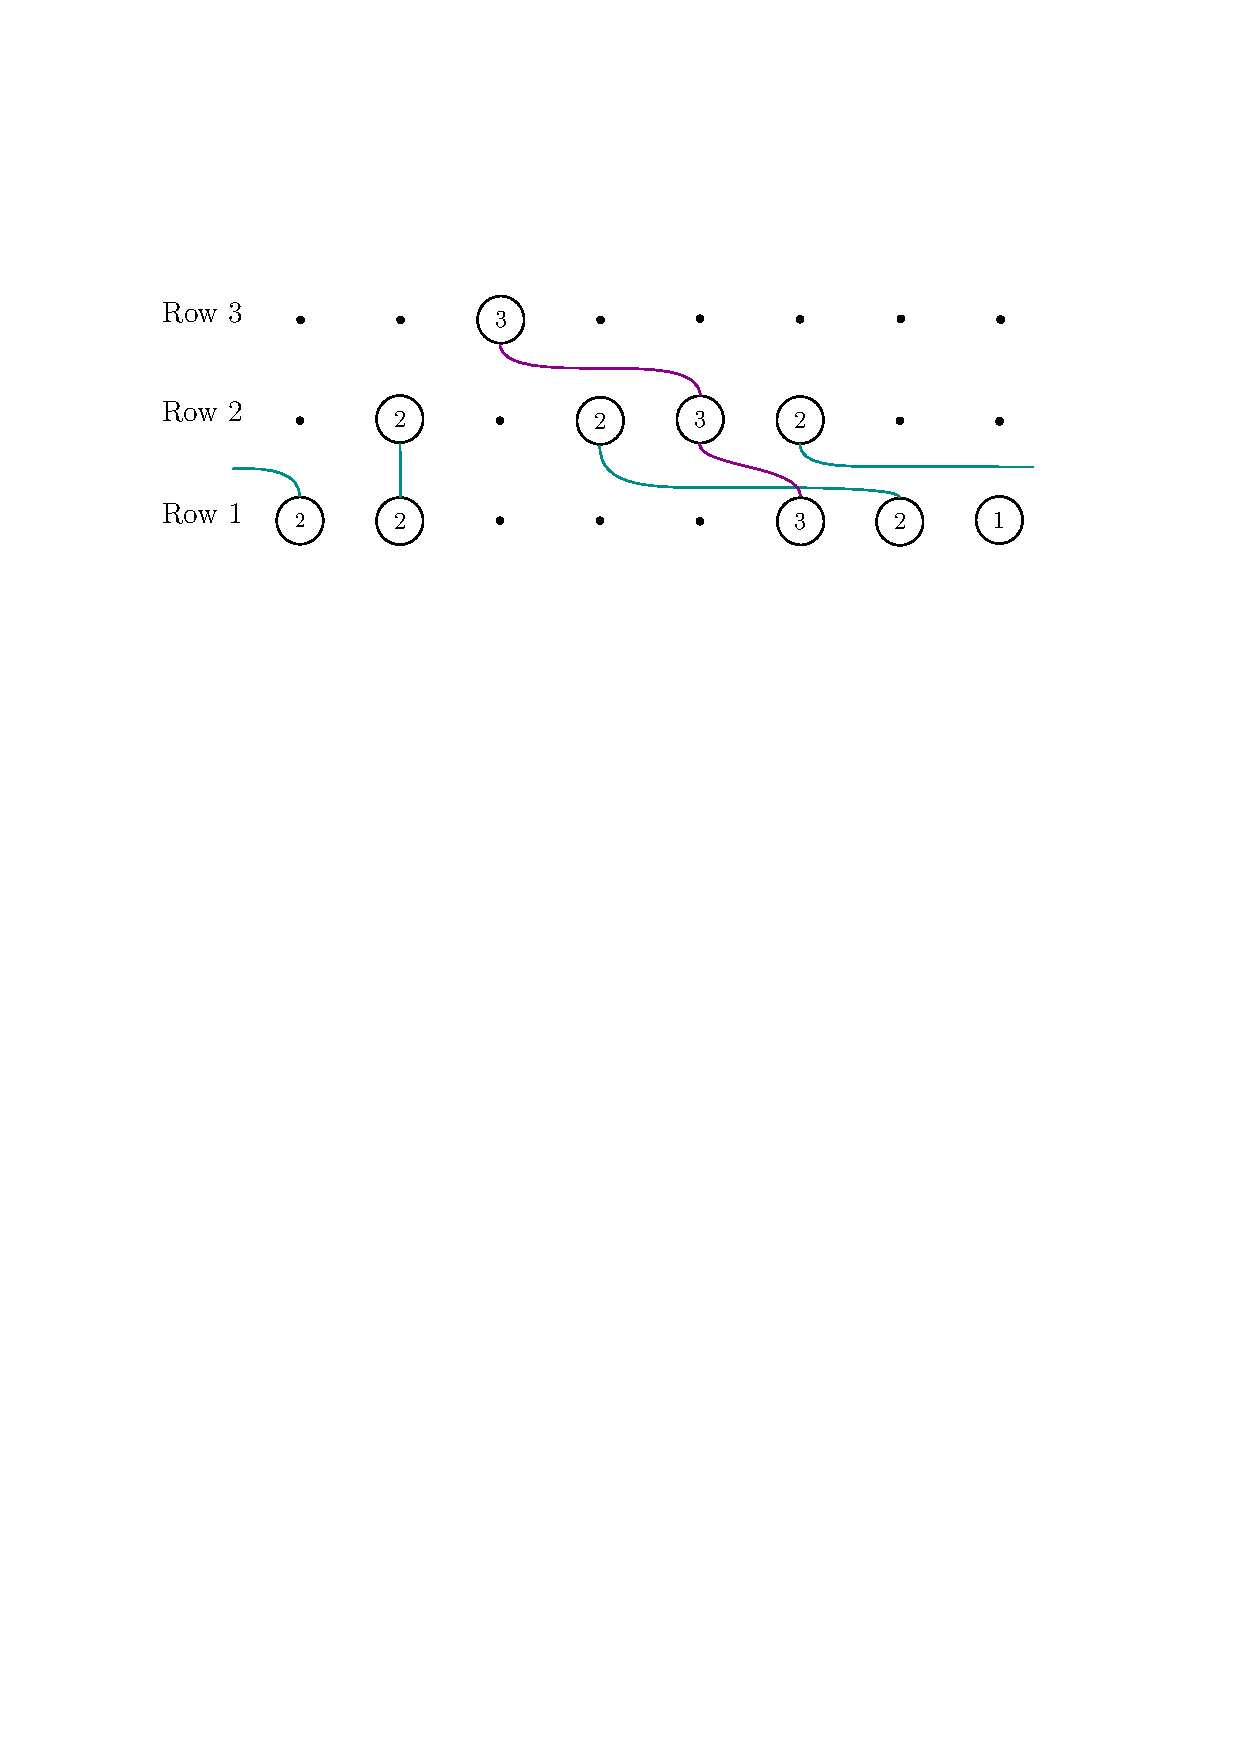
\includegraphics[width=0.5\linewidth]{MLQ.pdf}
    \caption*{A multiline queue.}
\end{figure}}

\only<2>{
\vspace{-0.6cm}
\begin{figure}
    \centering
    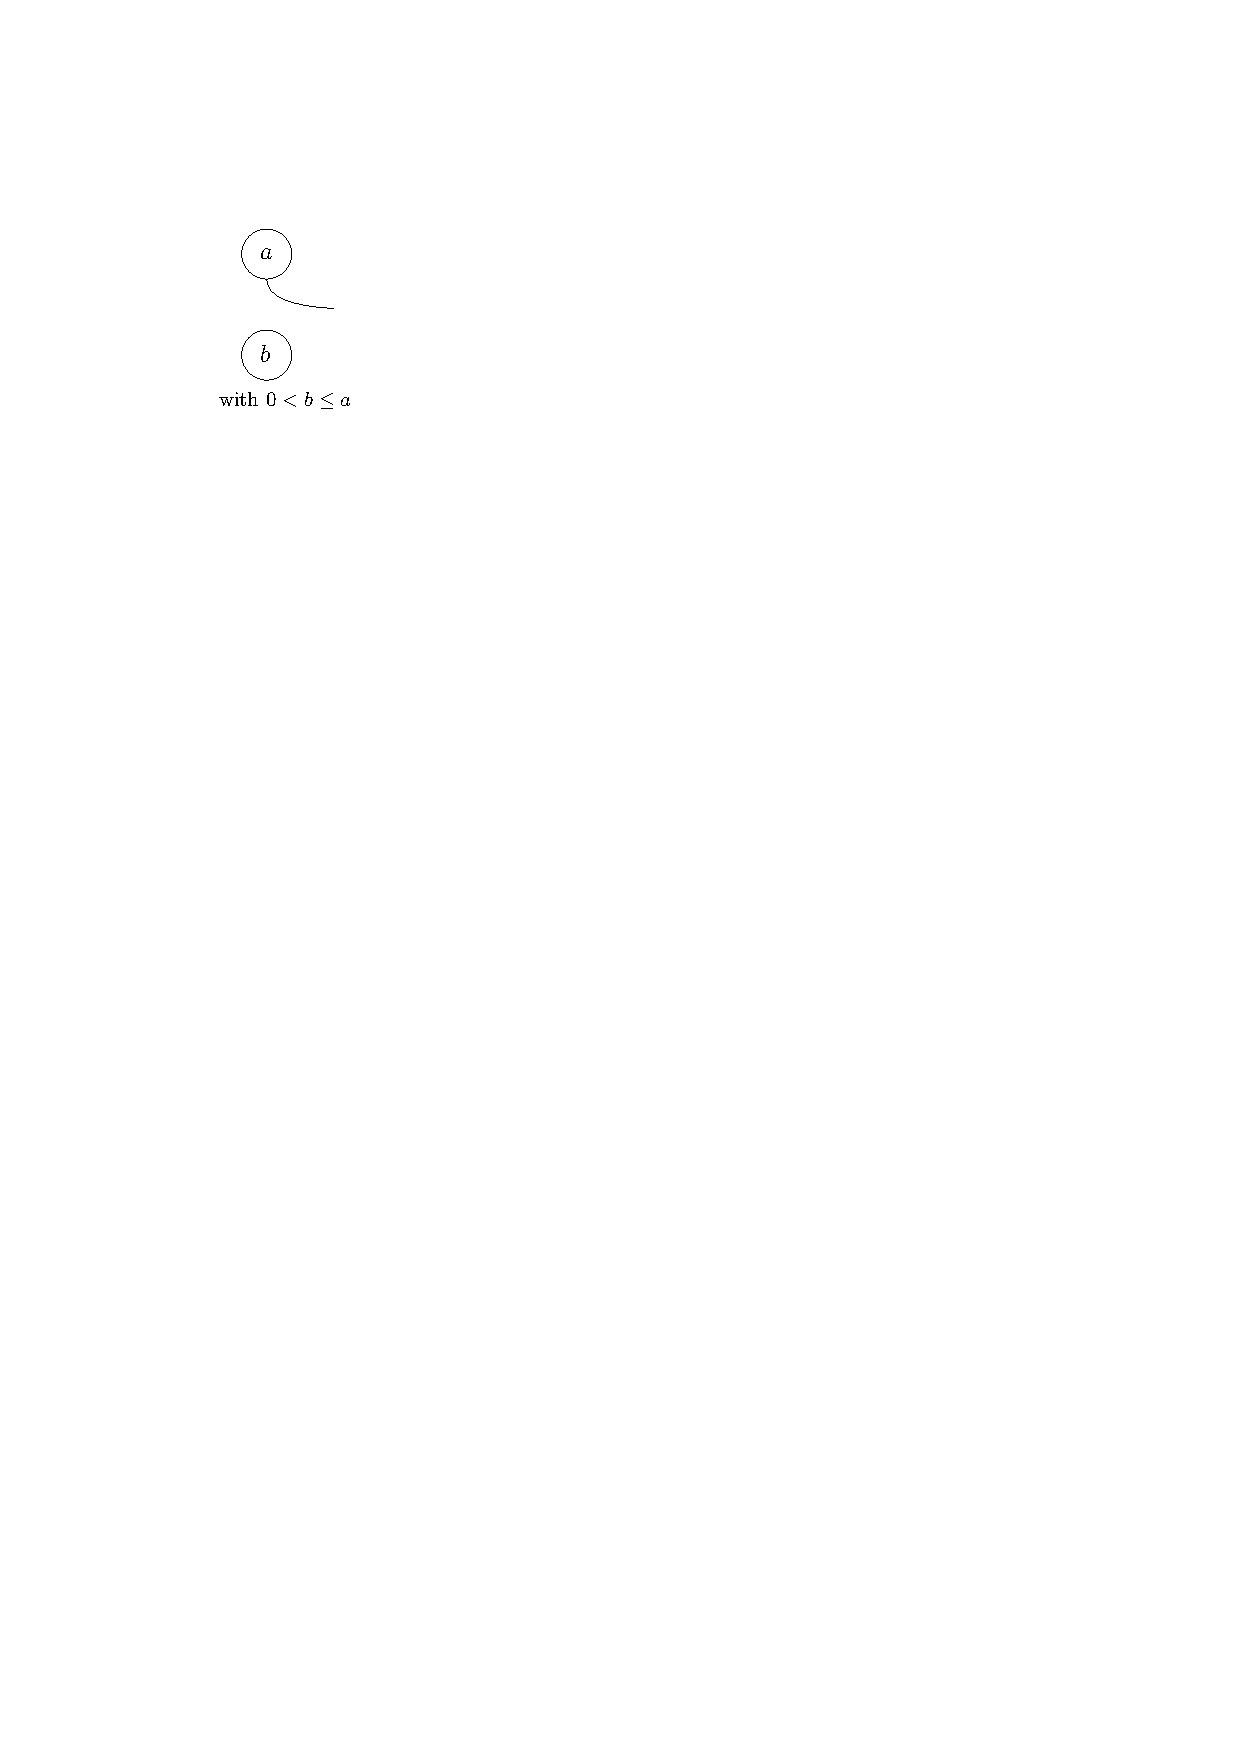
\includegraphics[width=0.11\linewidth]{Forbidden configuration classic0.pdf}
    \caption*{The forbidden configuration for multiline queues.}
\end{figure}}

\only<3>{
\begin{figure}
    \centering
    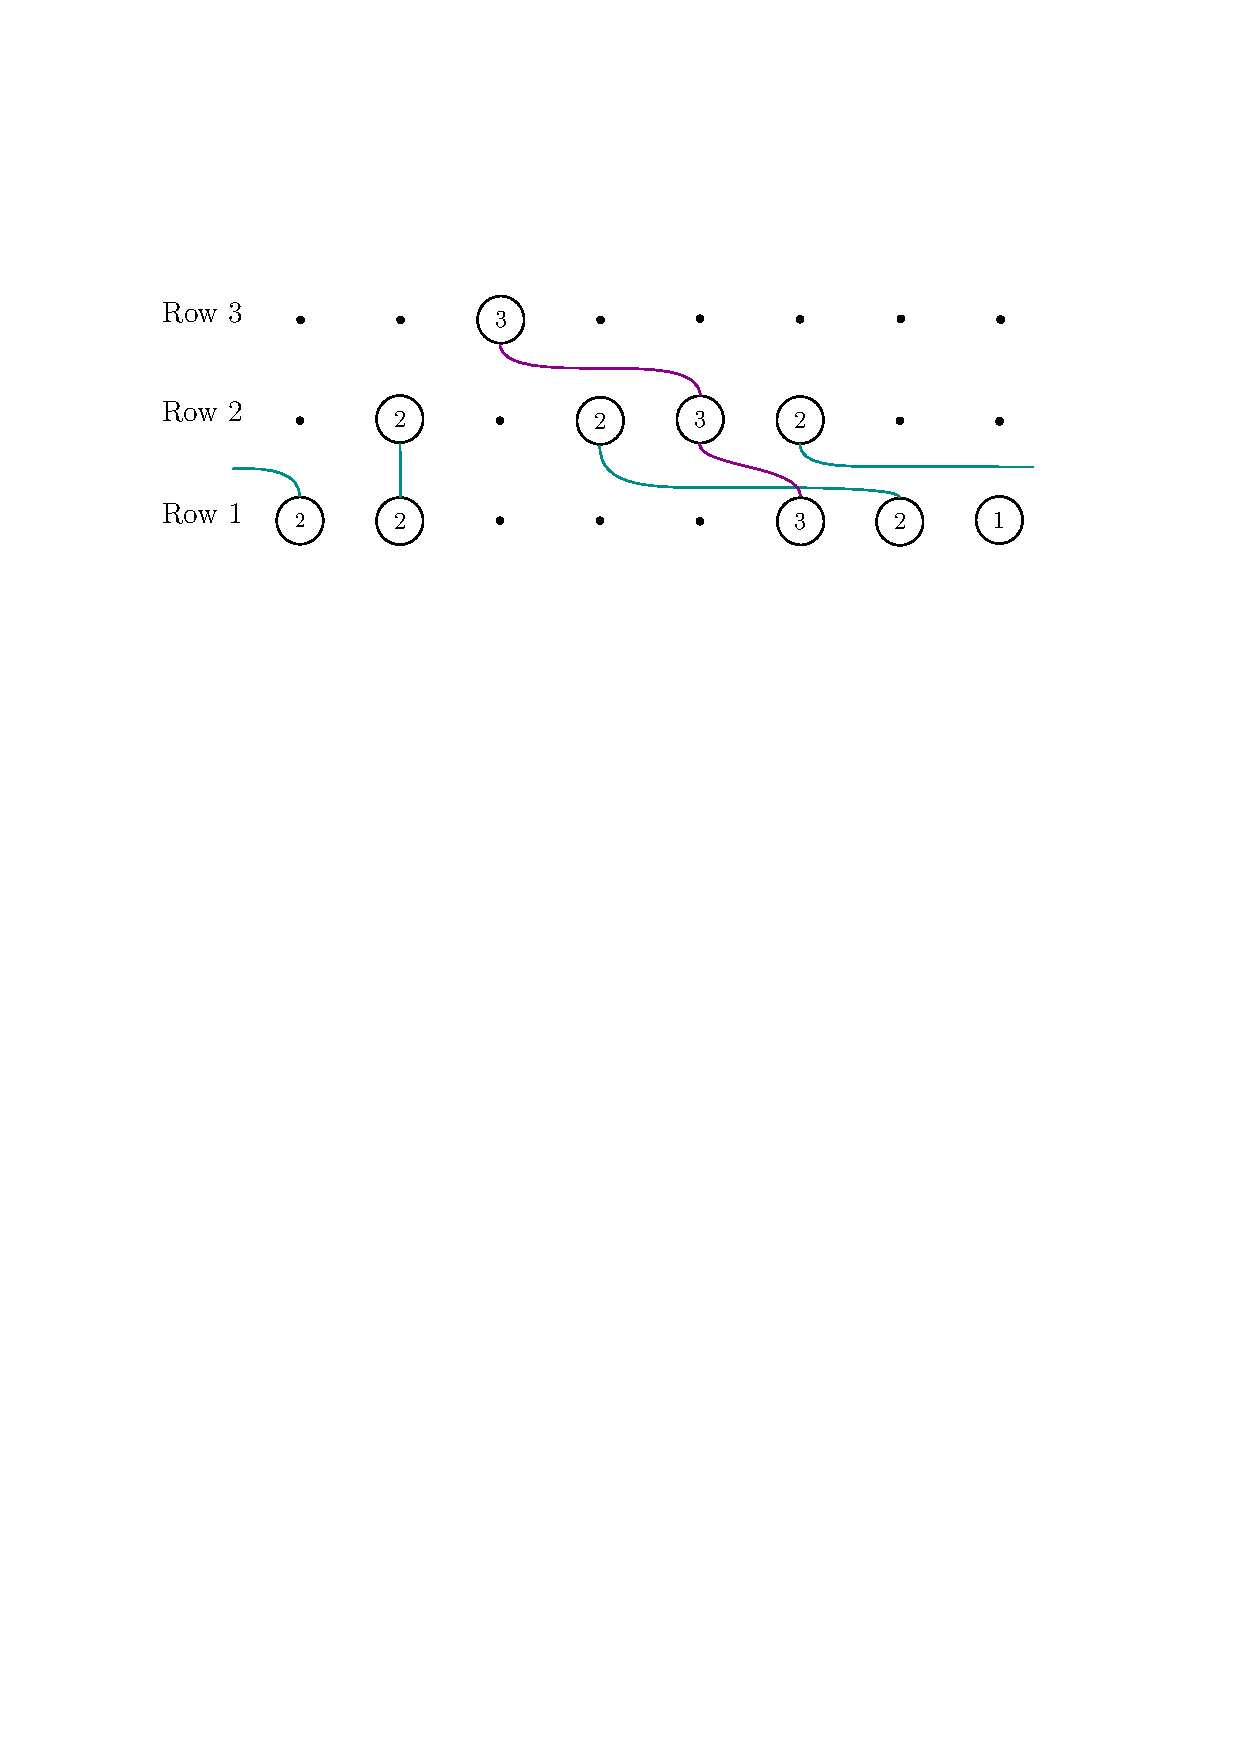
\includegraphics[width=0.5\linewidth]{MLQ.pdf}
    \caption*{A multiline queue of type $(2,2,0,0,0,3,2,1)$.}
\end{figure}
\vspace{-0.5cm}
The \textcolor{uibred}{type} of a multiline queue is the composition $\mu$ obtained by reading the labels in row 1.
\vspace{-0.5cm}
\begin{itemize}
    \item $n=\#\text{columns in the multiline queue}=\#\text{parts of $\mu$}.$
    \item $L=\#\text{rows in the multiline queue}=\text{the size of the maximal part in  $\mu$}.$
\end{itemize}
}

\end{frame}






\begin{frame}{Weights of Multiline queues}
\smaller
% \vspace{-0.5cm}
% \textbf{\textcolor{blue}{Weights:}}
\vspace{-0.2cm}
\textbf{\textcolor{blue}{Pairing order in each layer}:}

We read the balls in row $r$ in decreasing order of their label; 
within a fixed label $a$:
\begin{itemize}
    \item we start by placing the trivial $a$-pairings,
    \item we pair the remaining balls labeled $a$ from right to left.
\end{itemize}
  
As we read the balls in this order, we imagine placing the strands pairing the balls one by one.
\only<1>{\begin{figure}
    \centering
    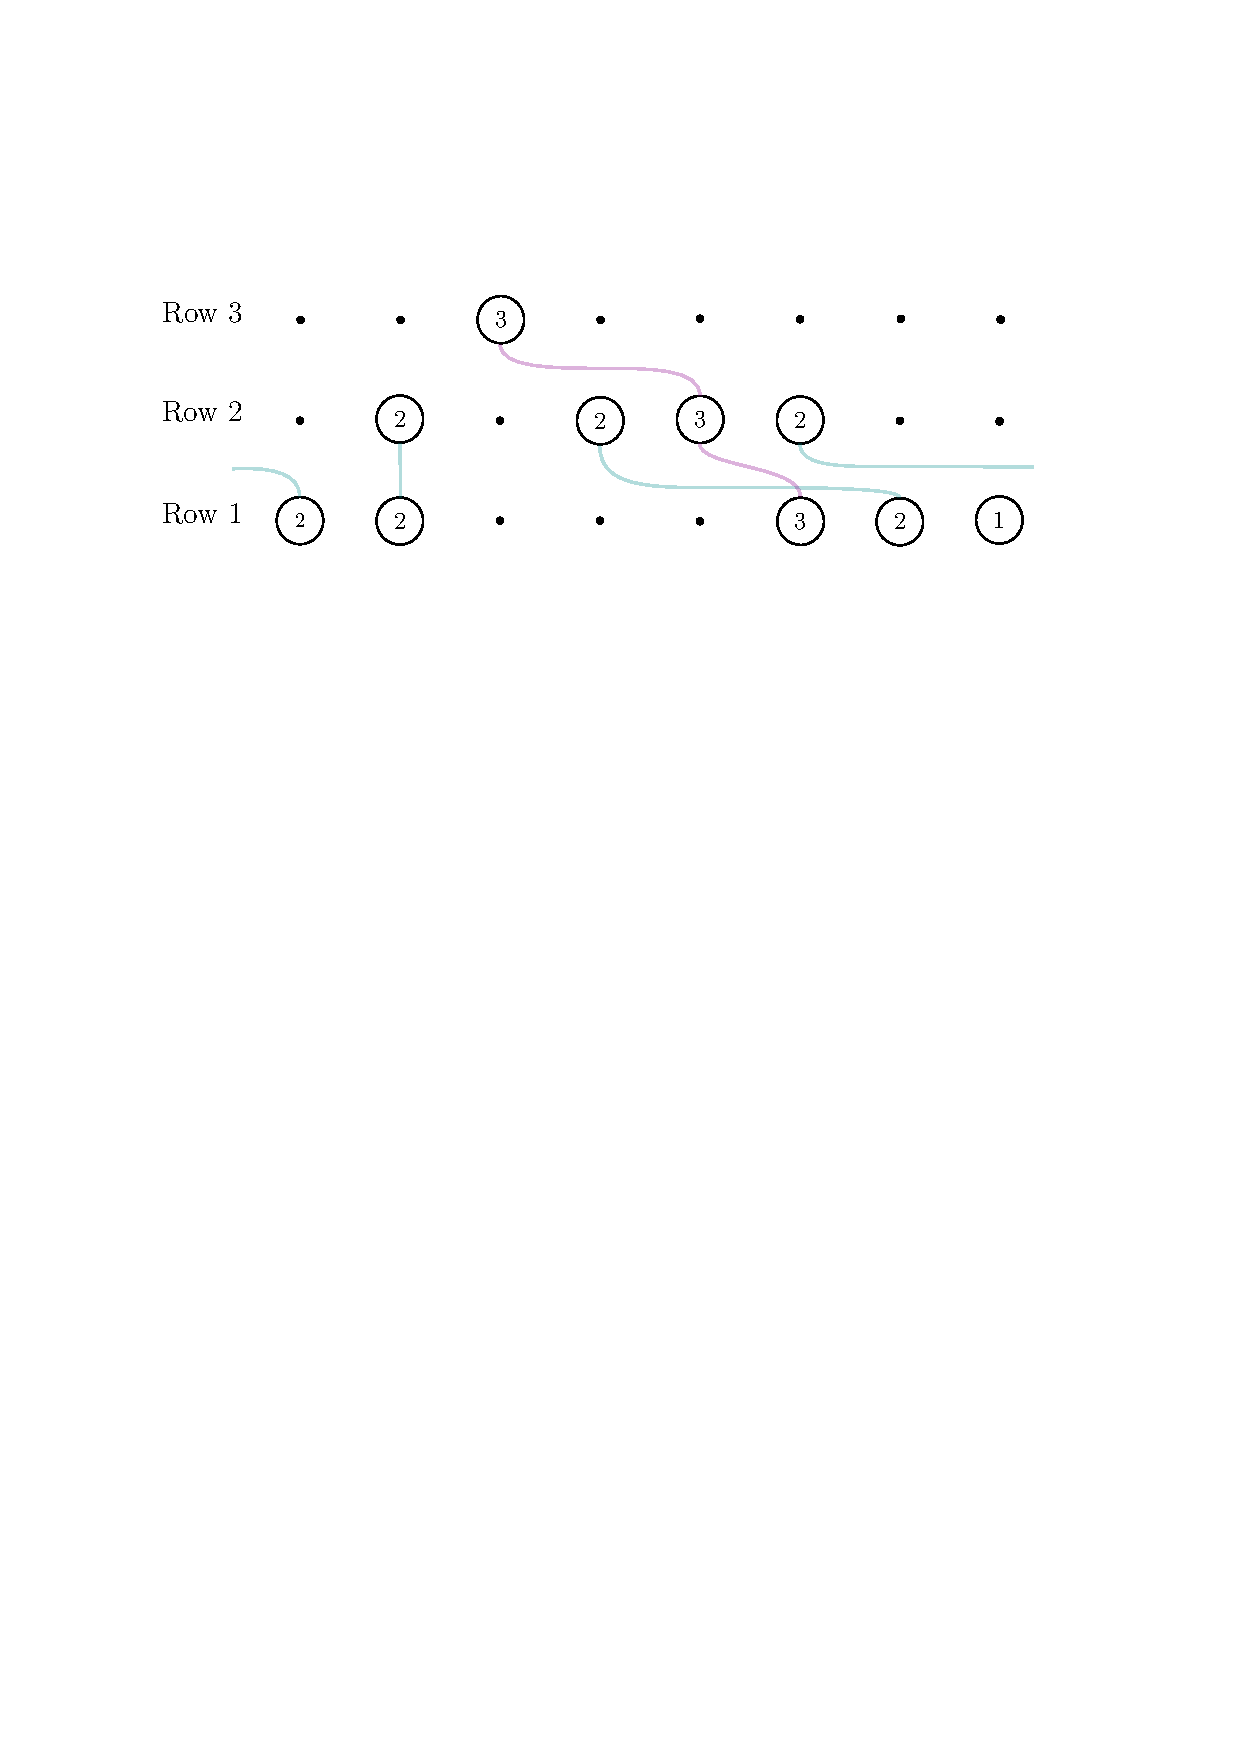
\includegraphics[width=0.5\linewidth]{MLQ0.pdf}
    \caption*{A multiline queue of type $(2,2,0,0,0,3,2,1)$.}
\end{figure}}


\only<2>{\begin{figure}
    \centering
    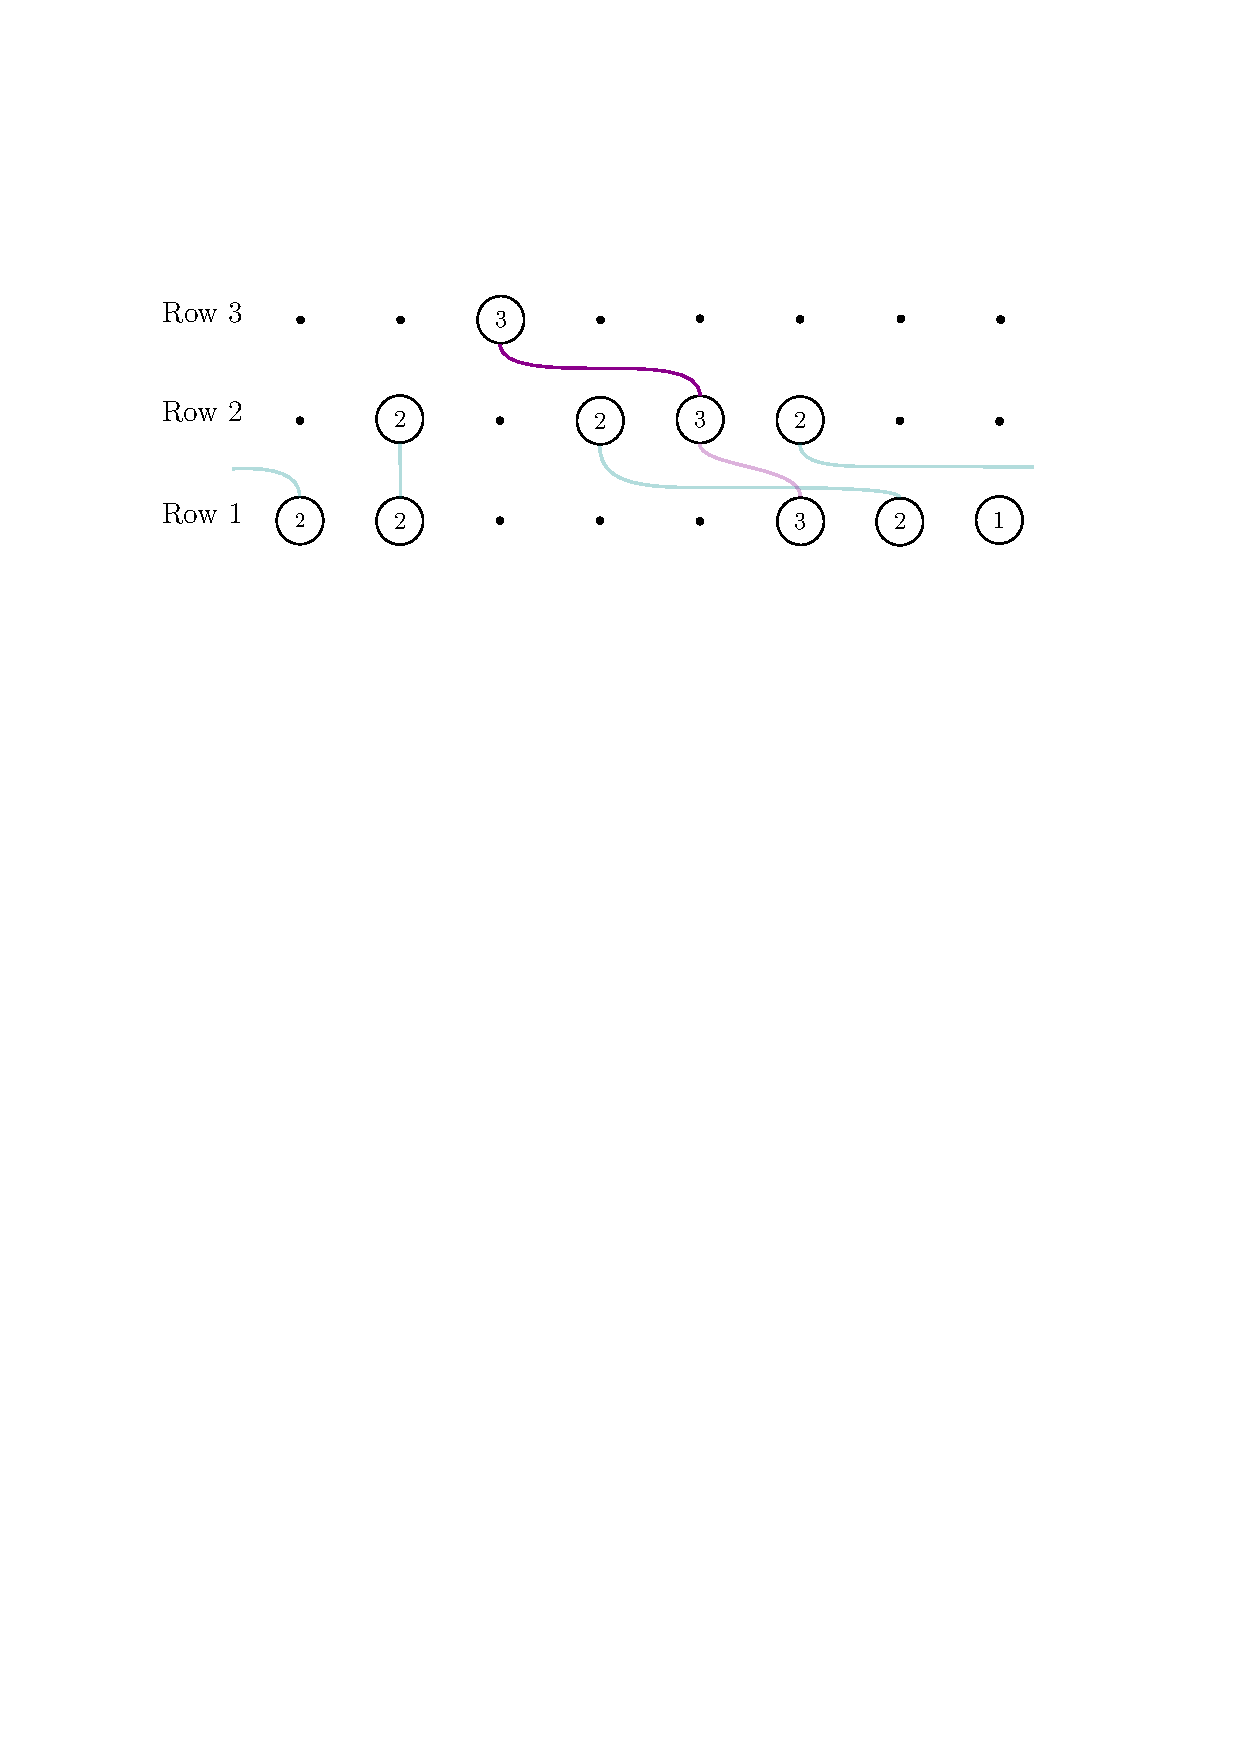
\includegraphics[width=0.5\linewidth]{MLQ1.pdf}
    \caption*{A multiline queue of type $(2,2,0,0,0,3,2,1)$.}
\end{figure}}

\only<3>{\begin{figure}
    \centering
    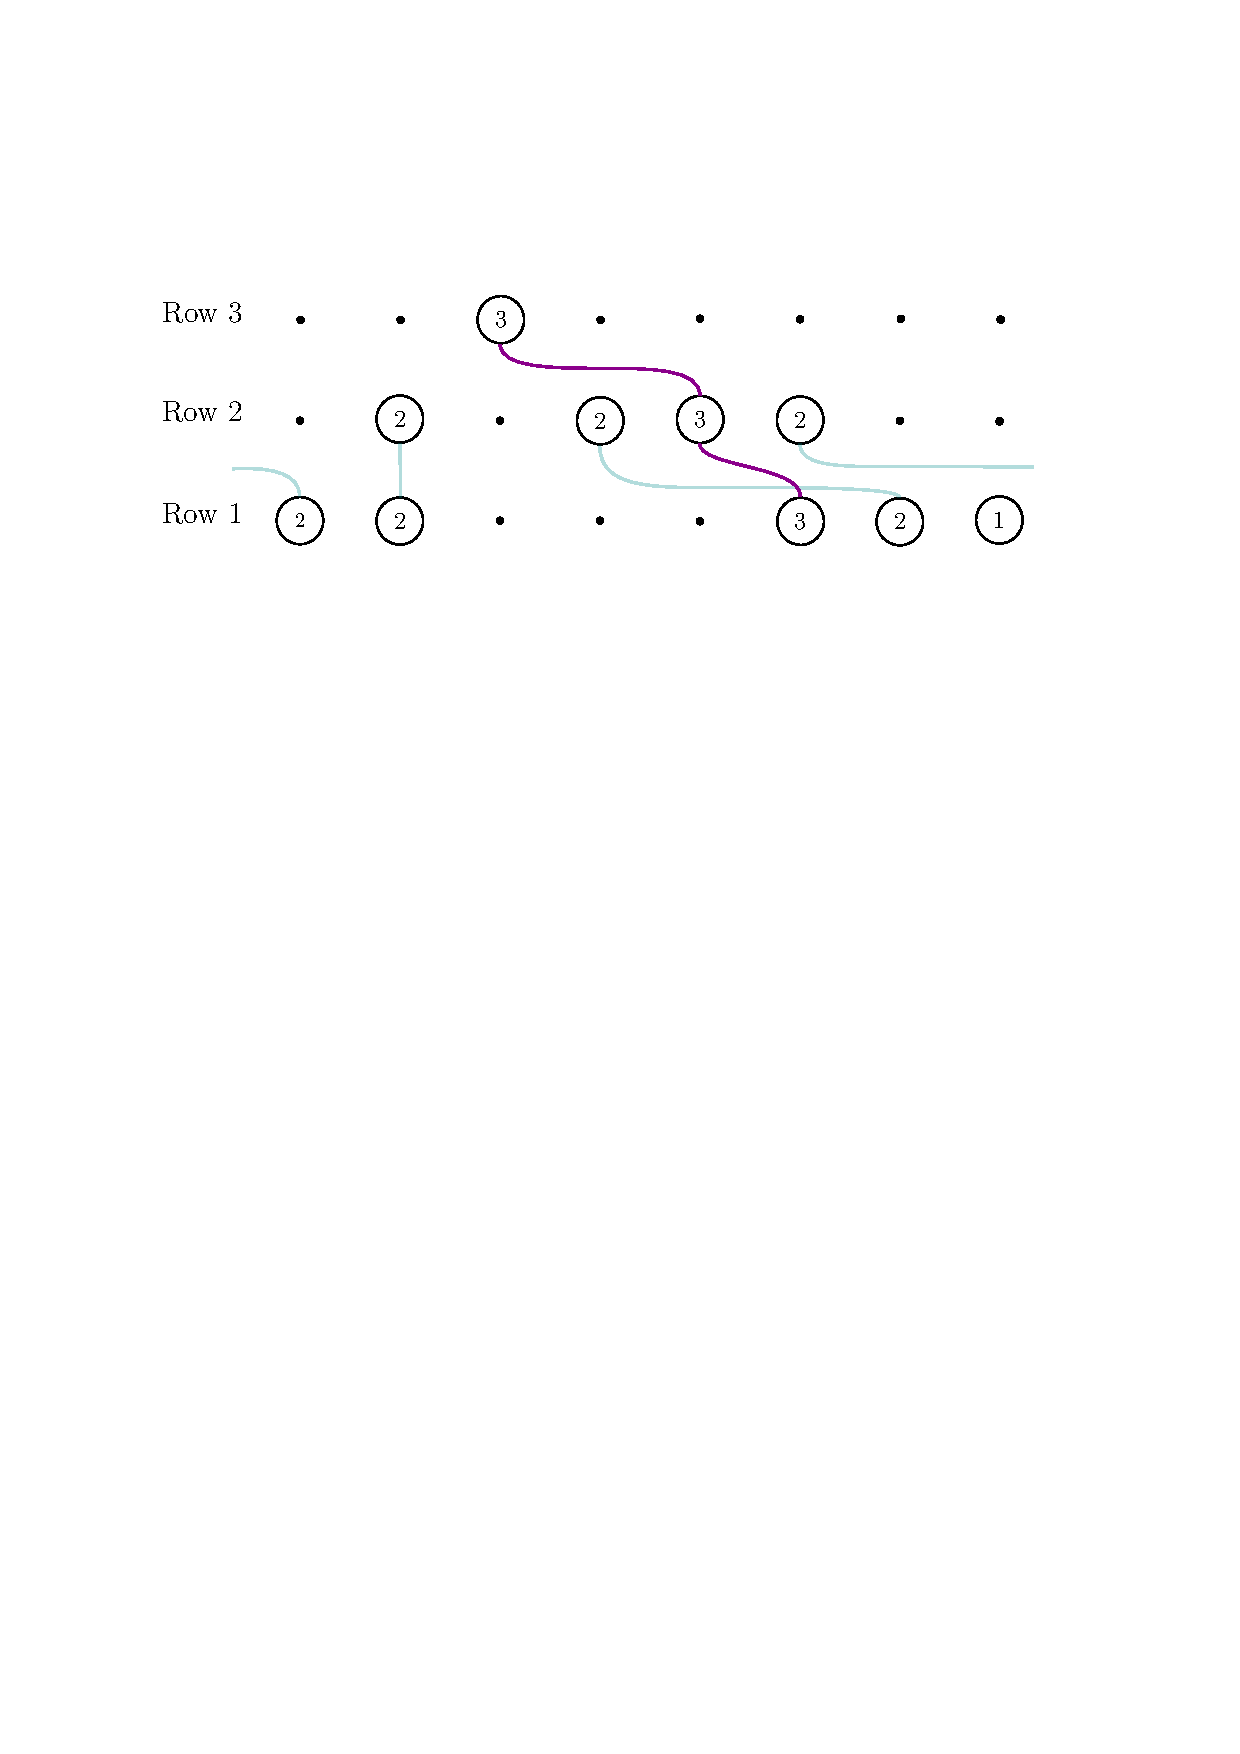
\includegraphics[width=0.5\linewidth]{MLQ2.pdf}
    \caption*{A multiline queue of type $(2,2,0,0,0,3,2,1)$.}
\end{figure}}

\only<4>{\begin{figure}
    \centering
    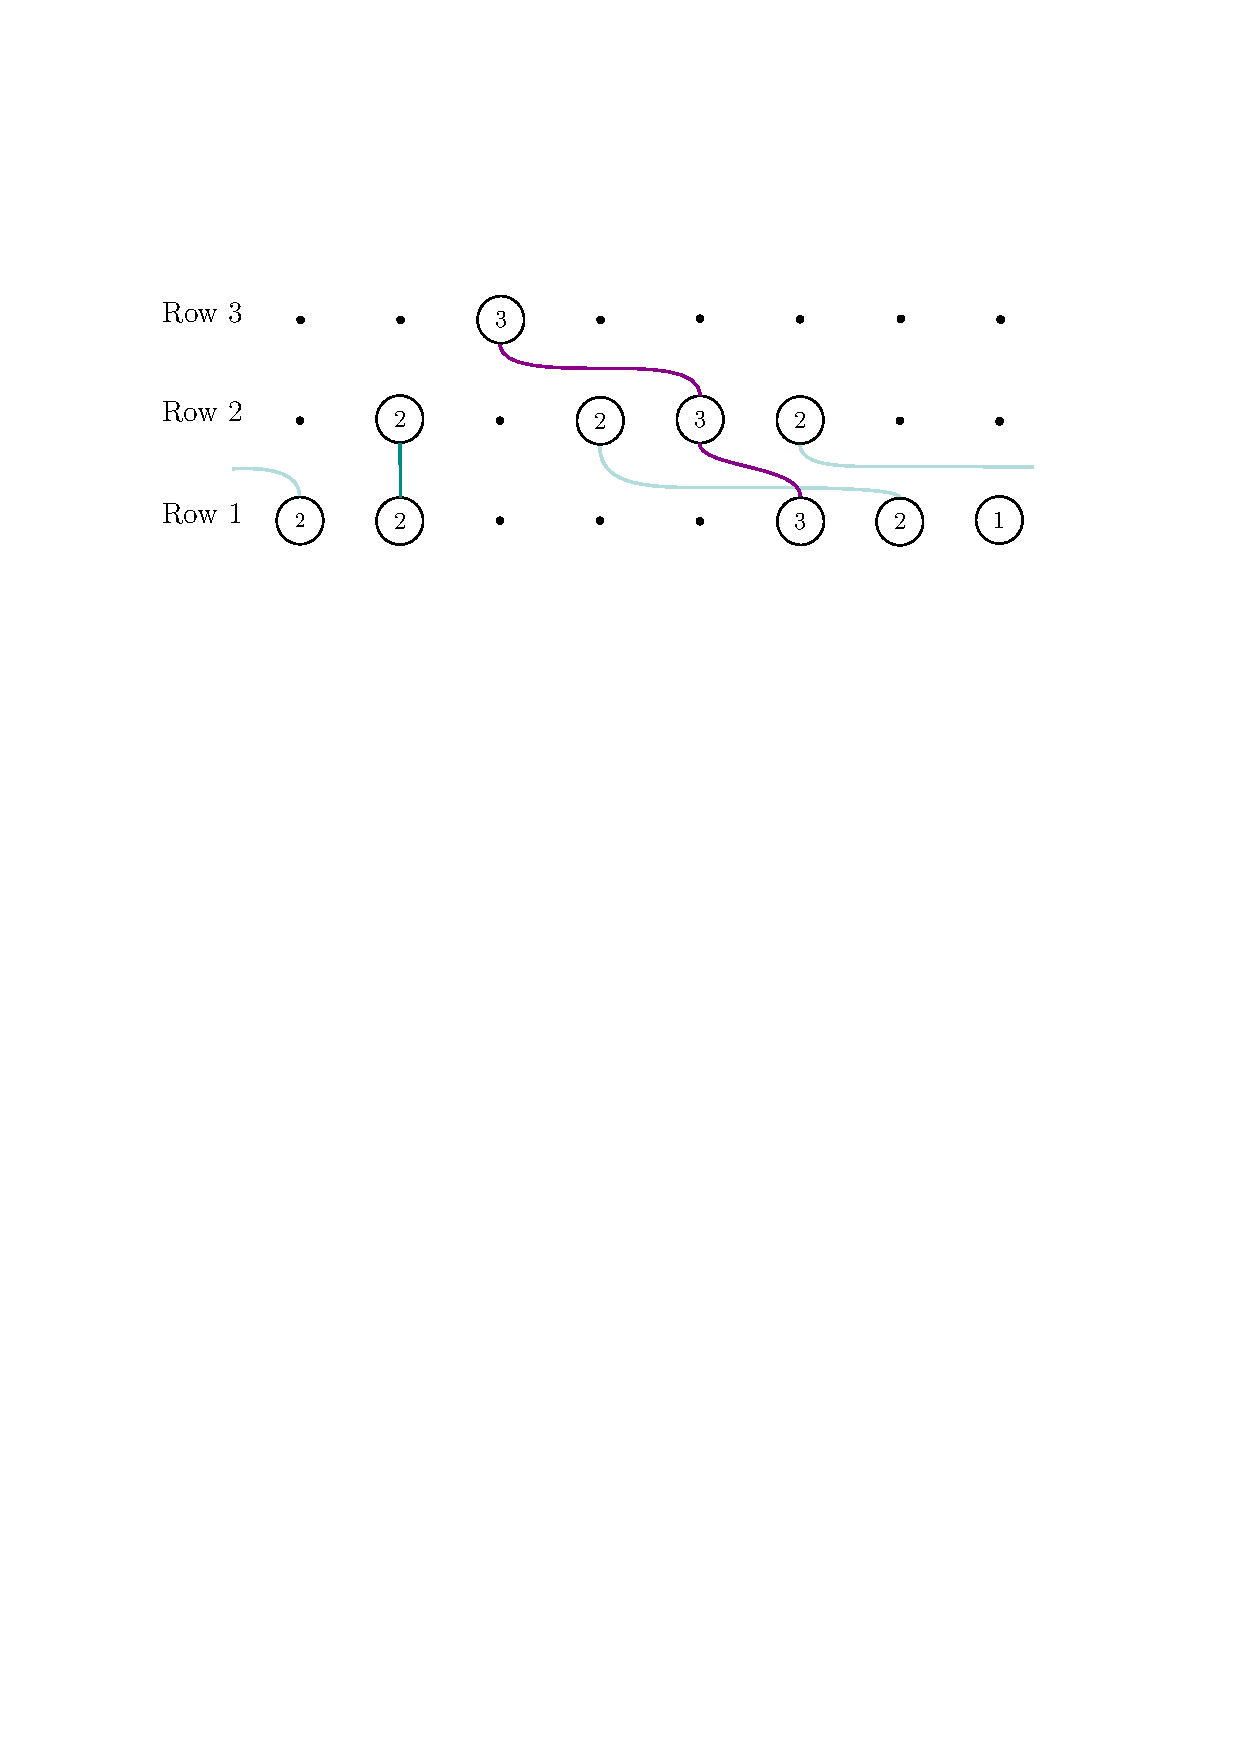
\includegraphics[width=0.5\linewidth]{MLQ3.pdf}
    \caption*{A multiline queue of type $(2,2,0,0,0,3,2,1)$.}
\end{figure}}

\only<5>{\begin{figure}
    \centering
    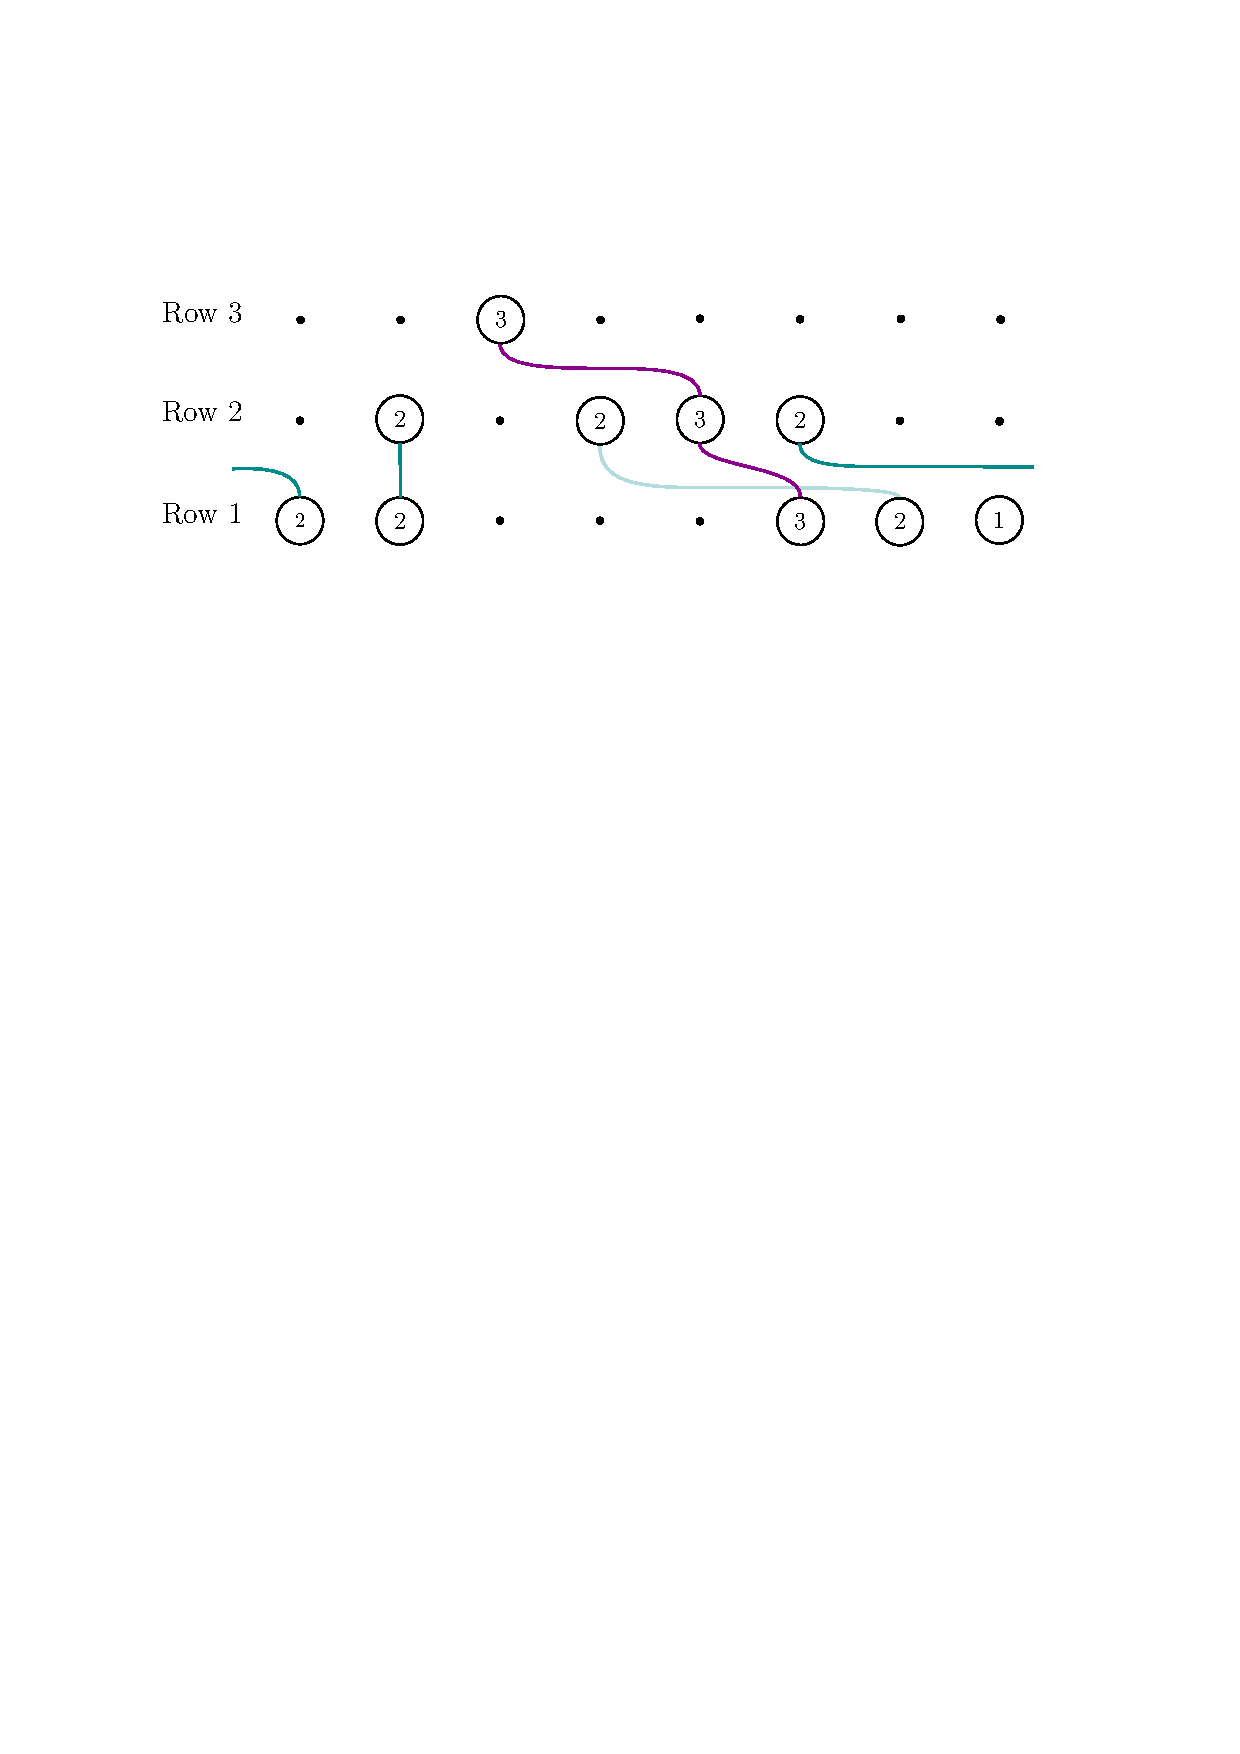
\includegraphics[width=0.5\linewidth]{MLQ4.pdf}
    \caption*{A multiline queue of type $(2,2,0,0,0,3,2,1)$.}
\end{figure}}


\only<6>{\begin{figure}
    \centering
    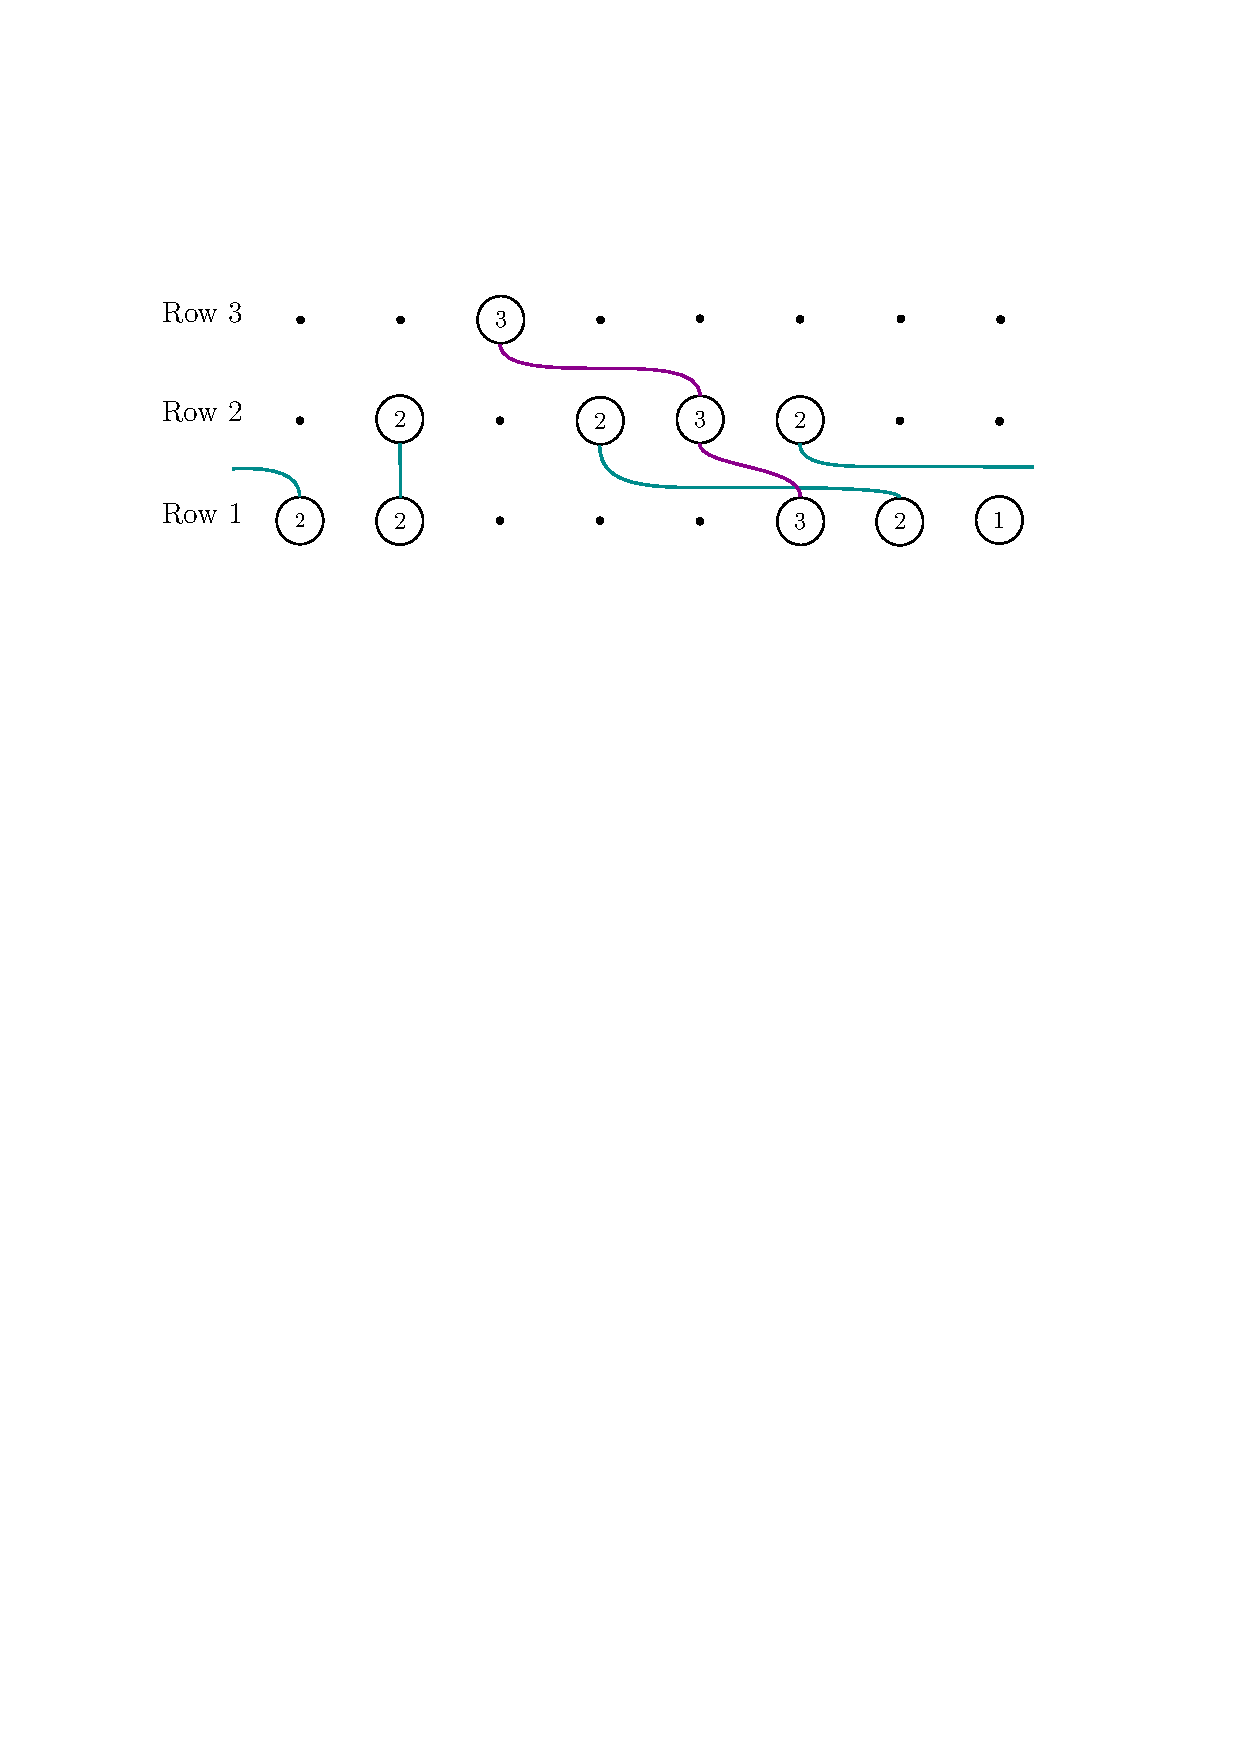
\includegraphics[width=0.5\linewidth]{MLQ5.pdf}
    \caption*{A multiline queue of type $(2,2,0,0,0,3,2,1)$.}
\end{figure}}


\end{frame}


\begin{frame}{Weights of Multiline queues}
\smaller
% \vspace{-0.5cm}
% \textbf{\textcolor{blue}{Weights:}}
\vspace{-0.2cm}
\begin{itemize}
    \item A ball in column $i$ has the weight $x_i$.
    \item Each nontrivial pairing $p$, connecting balls labeled $a$, between rows $r>1$ and $r-1$, and columns $j$ and $j'$, has weight $\wt_{\textup{pair}}(p)$: 
    
\begin{align*}\label{eq:pair}
\wt_{\pair}(p) = \begin{cases}
\frac{(1-t) t^{\skipped(p)}}{1-q^{a-r+1}t^{\free(p)}}
&\mbox{if $j'>j$}\\
\frac{(1-t) t^{\skipped(p)}}{1-q^{a-r+1}t^{\free(p)}}\cdot q^{a-r+1}
&\mbox {if $j'<j$}.
\end{cases}
\end{align*}
$\free(p):$ balls not yet paired in row $r-1$,\\
$\skipped(p)$: free balls which have been skipped by $p$.

\begin{figure}
    \centering
    \begin{subfigure}{0.45\textwidth}
        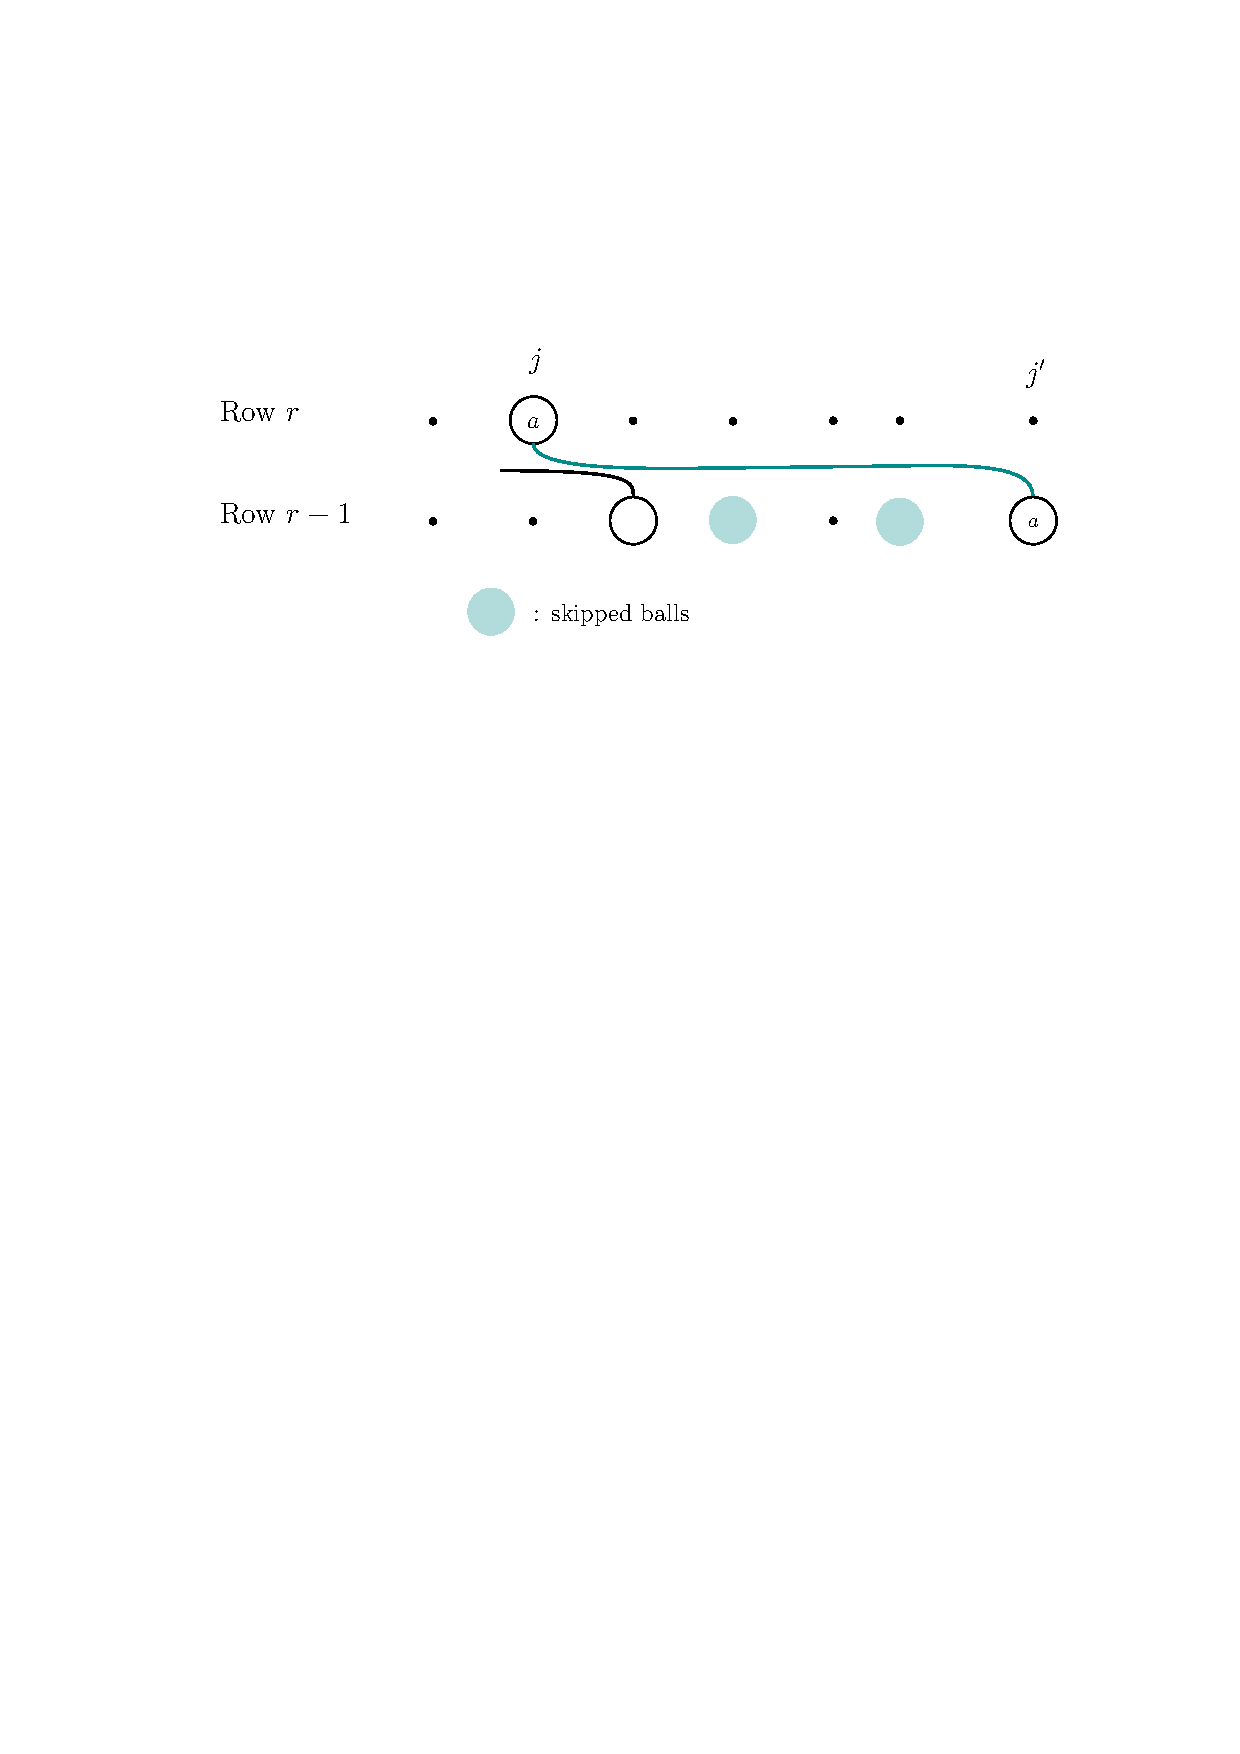
\includegraphics[width=1.14\linewidth]{Not wrapped Pairings.pdf}
    \subcaption*{Case $j<j'$}
    \end{subfigure}
    \begin{subfigure}{0.45\textwidth}
    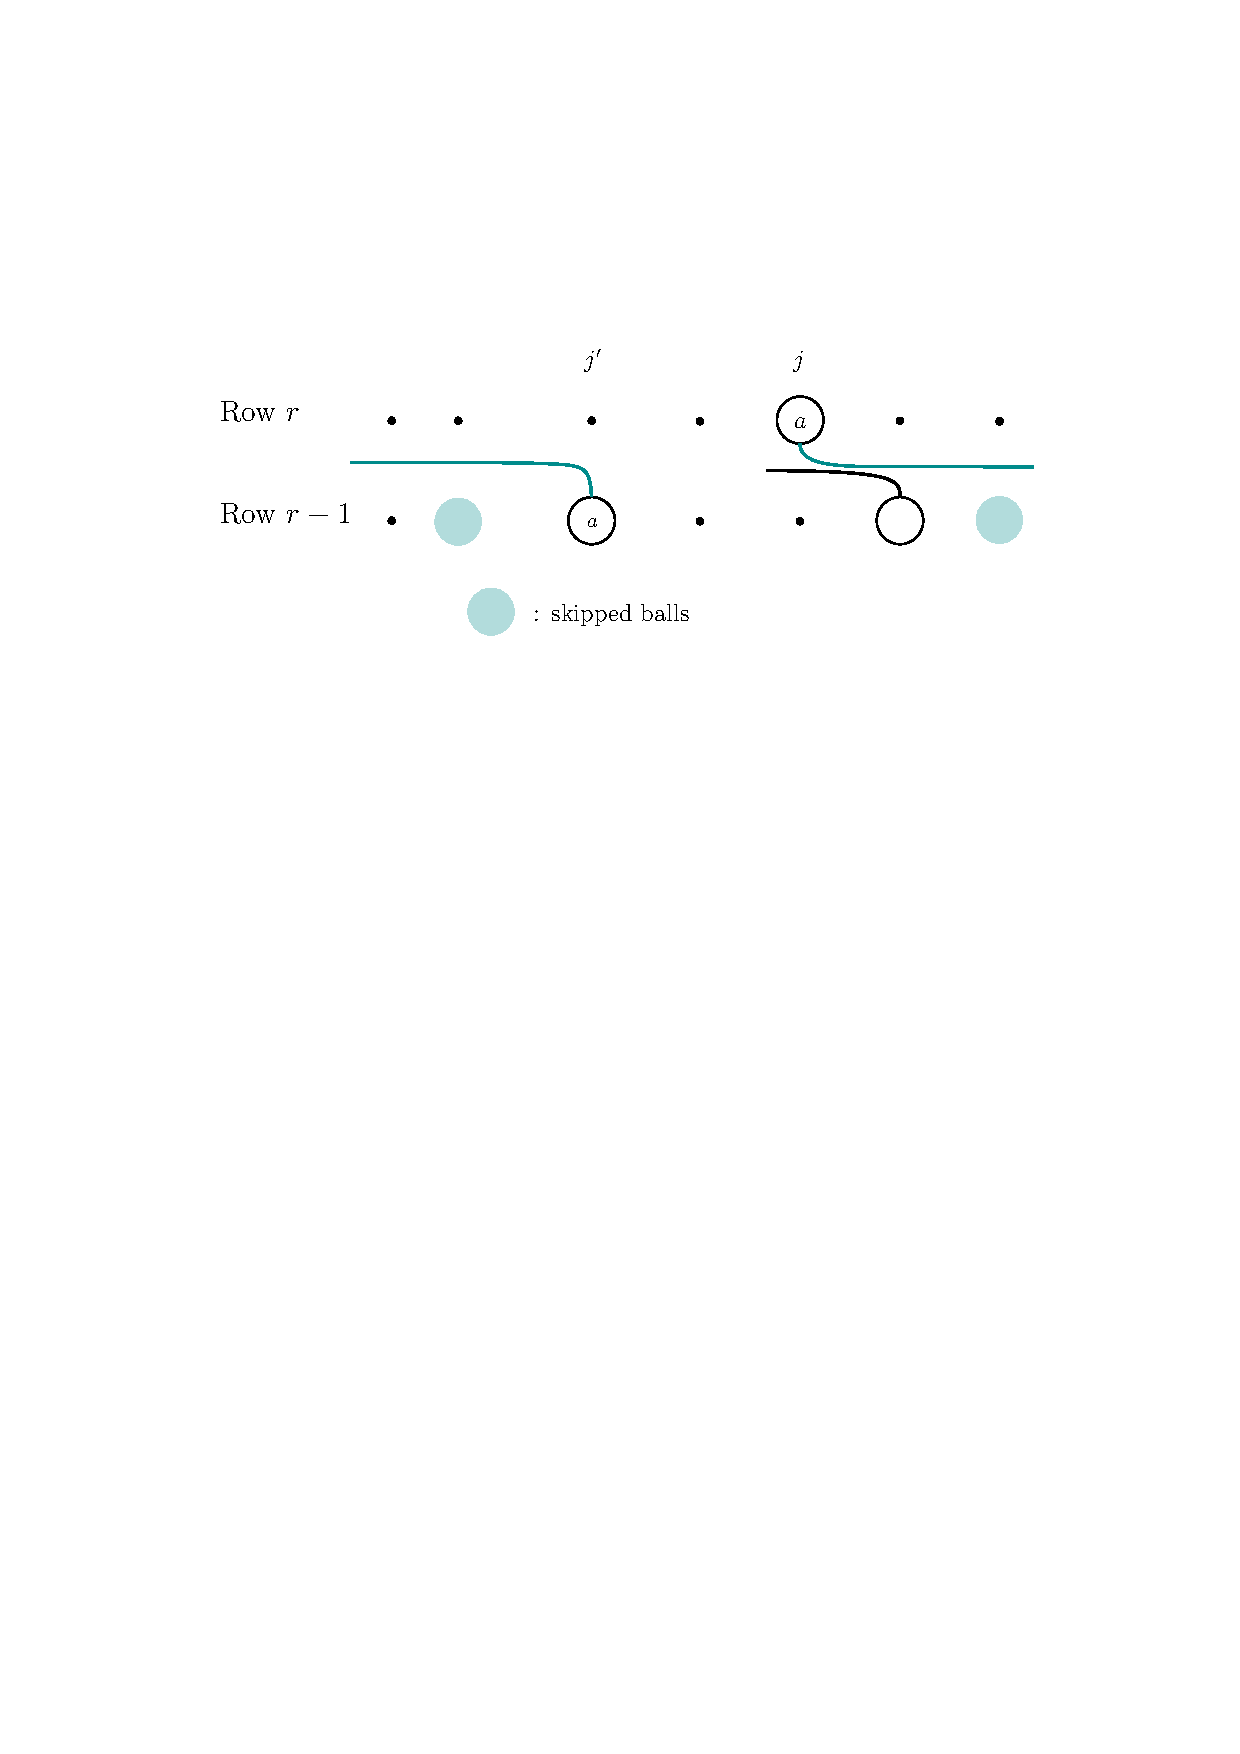
\includegraphics[width=1.14\linewidth]{Pairings.pdf}
    \subcaption*{Case $j>j'$}
    \end{subfigure}
\end{figure}

    \item The total weight of a multiline queue $Q$ is denoted $\wt(Q)$:
    $$\wt(Q) = \prod_{\text{balls $B$}}\wt(B) \prod_{\text{pairings}\ p} \wt_{\pair}(p).$$

    
\end{itemize}

\end{frame}

\begin{frame}{Weights of Multiline queues}
\smaller
% \vspace{-0.5cm}
% \textbf{\textcolor{blue}{Weights:}}
\vspace{-0.2cm}
\begin{itemize}
    \item A ball in column $i$ has the weight $x_i$.
    \item Each nontrivial pairing $p$ has weight $\wt_{\textup{pair}}(p)$:
\begin{align*}
\wt_{\pair}(p) = \begin{cases}
\frac{(1-t) t^{\skipped(p)}}{1-q^{a-r+1}t^{\free(p)}}
&\mbox{if $j'>j$}\\
\frac{(1-t) t^{\skipped(p)}}{1-q^{a-r+1}t^{\free(p)}}\cdot q^{a-r+1}
&\mbox {if $j'<j$}.
\end{cases}
\end{align*}

\item The total weight of a multiline queue $Q$ is denoted $\wt(Q)$.
\end{itemize}
\vspace{-0.5cm}

\textbf{\textcolor{blue}{Example:}}
\only<1>{\begin{figure}
    \centering
    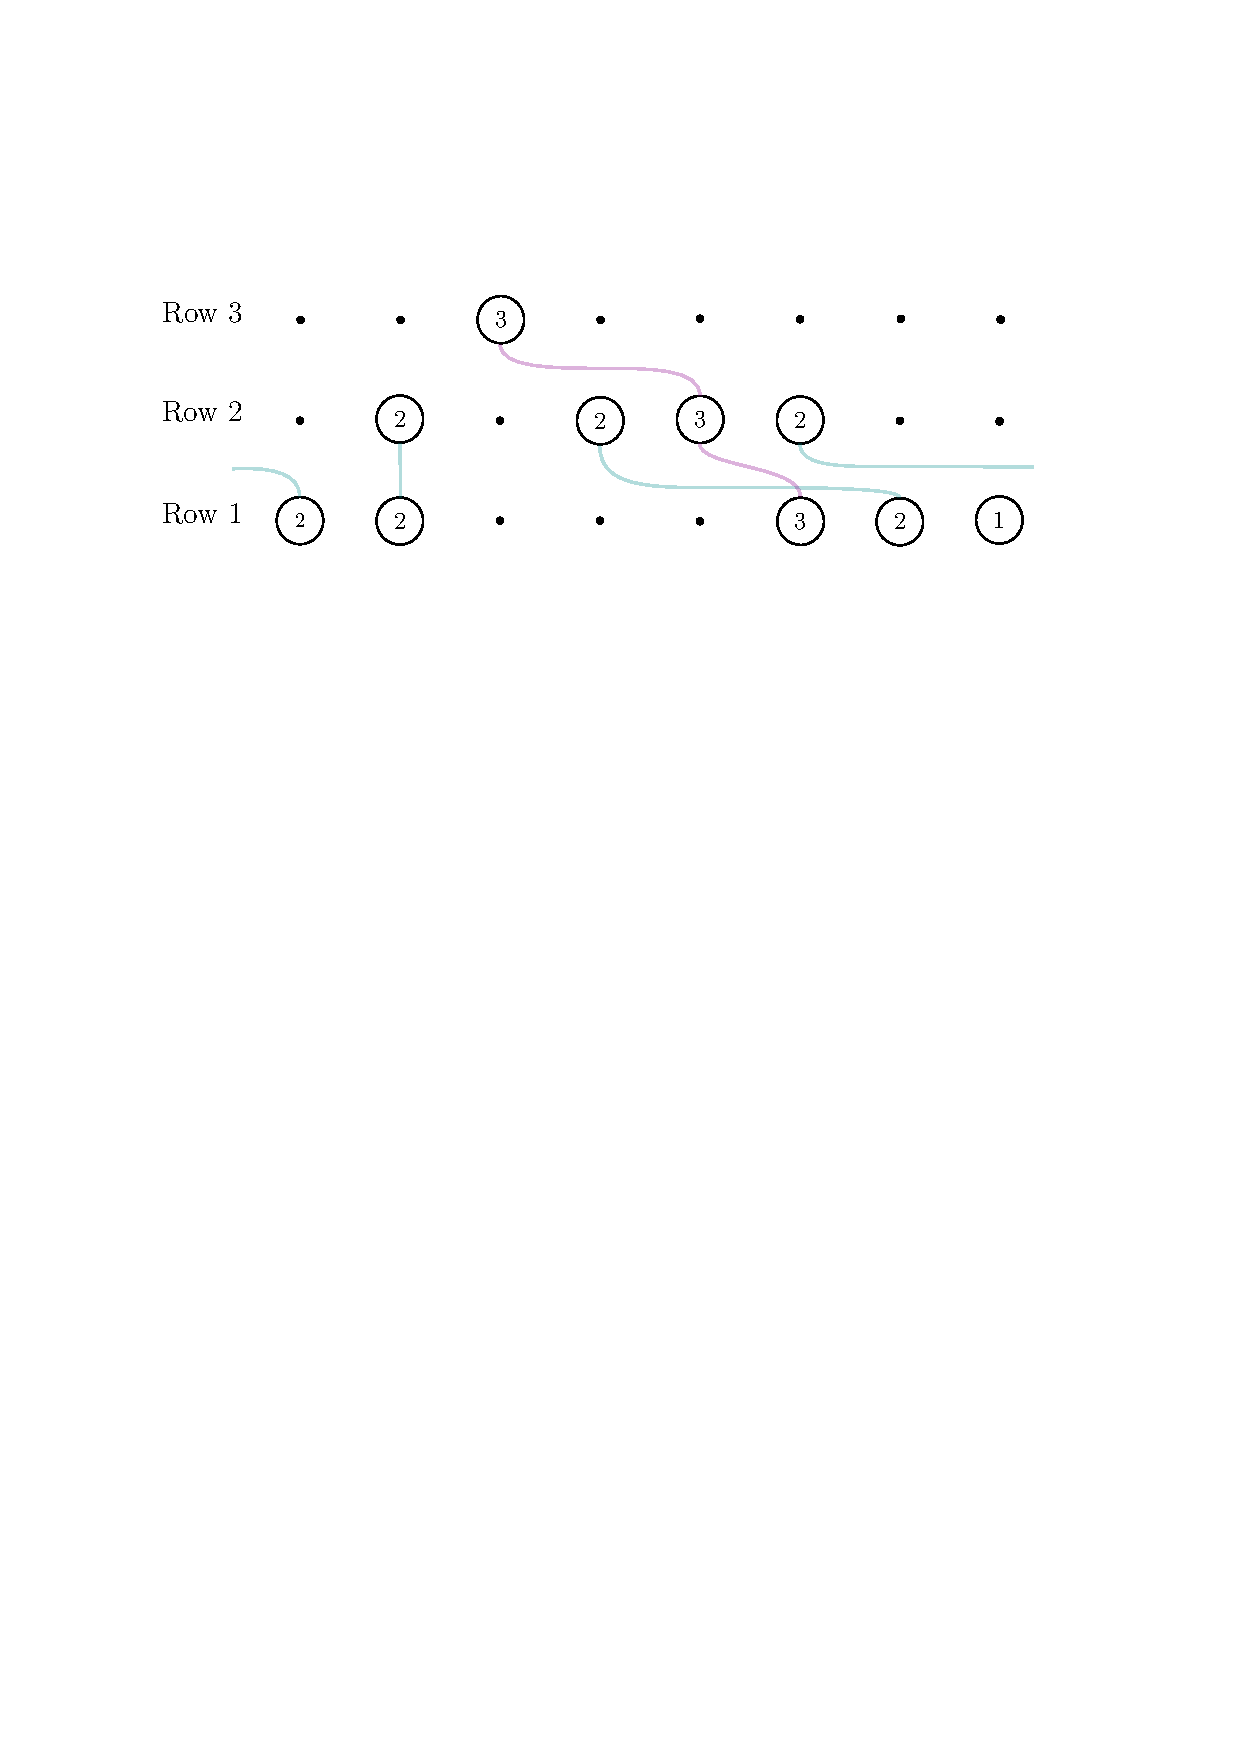
\includegraphics[width=0.5\linewidth]{MLQ0.pdf}
    \caption*{A multiline queue of type $(2,2,0,0,0,3,2,1)$.}
\end{figure}}


\only<2>{\begin{figure}
    \centering
    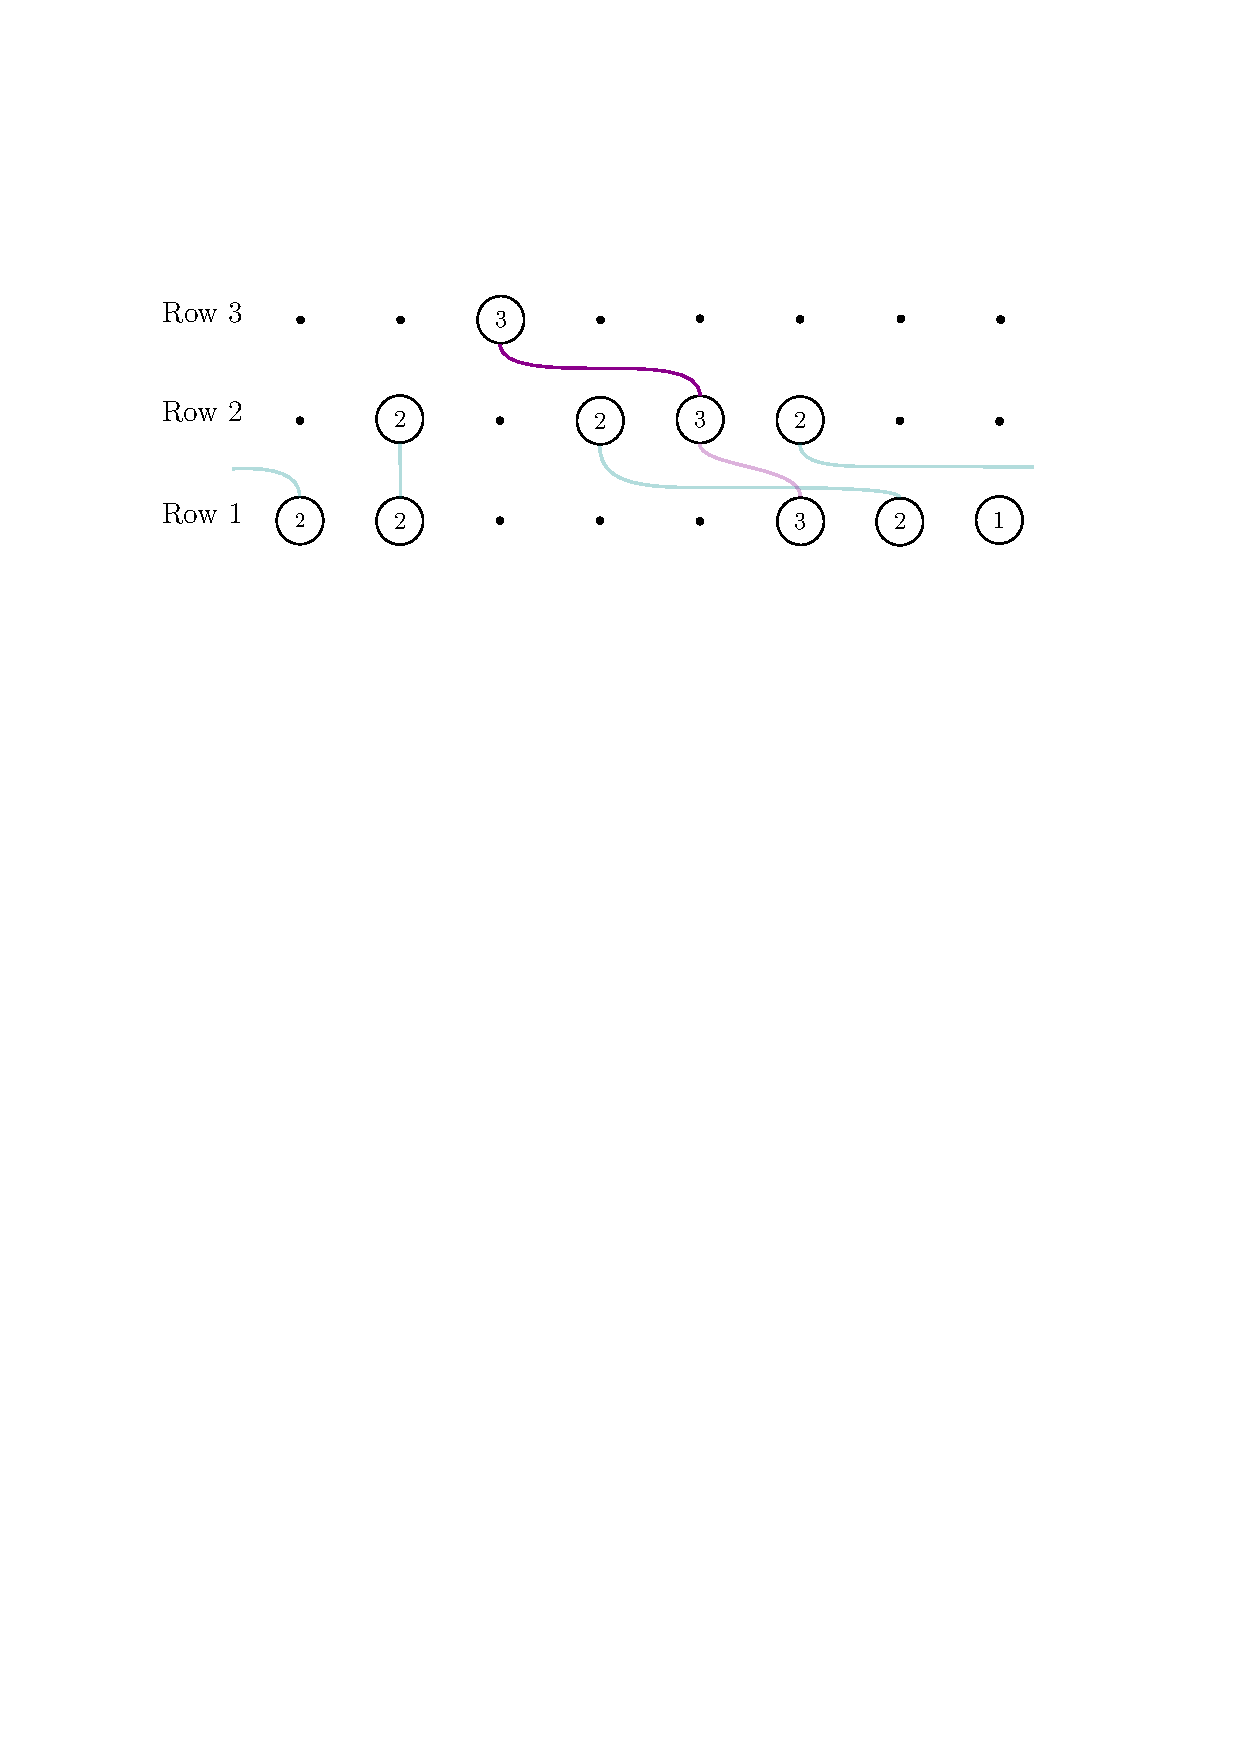
\includegraphics[width=0.5\linewidth]{MLQ1.pdf}
    \caption*{A multiline queue of type $(2,2,0,0,0,3,2,1)$.}
\end{figure}}

\only<3>{\begin{figure}
    \centering
    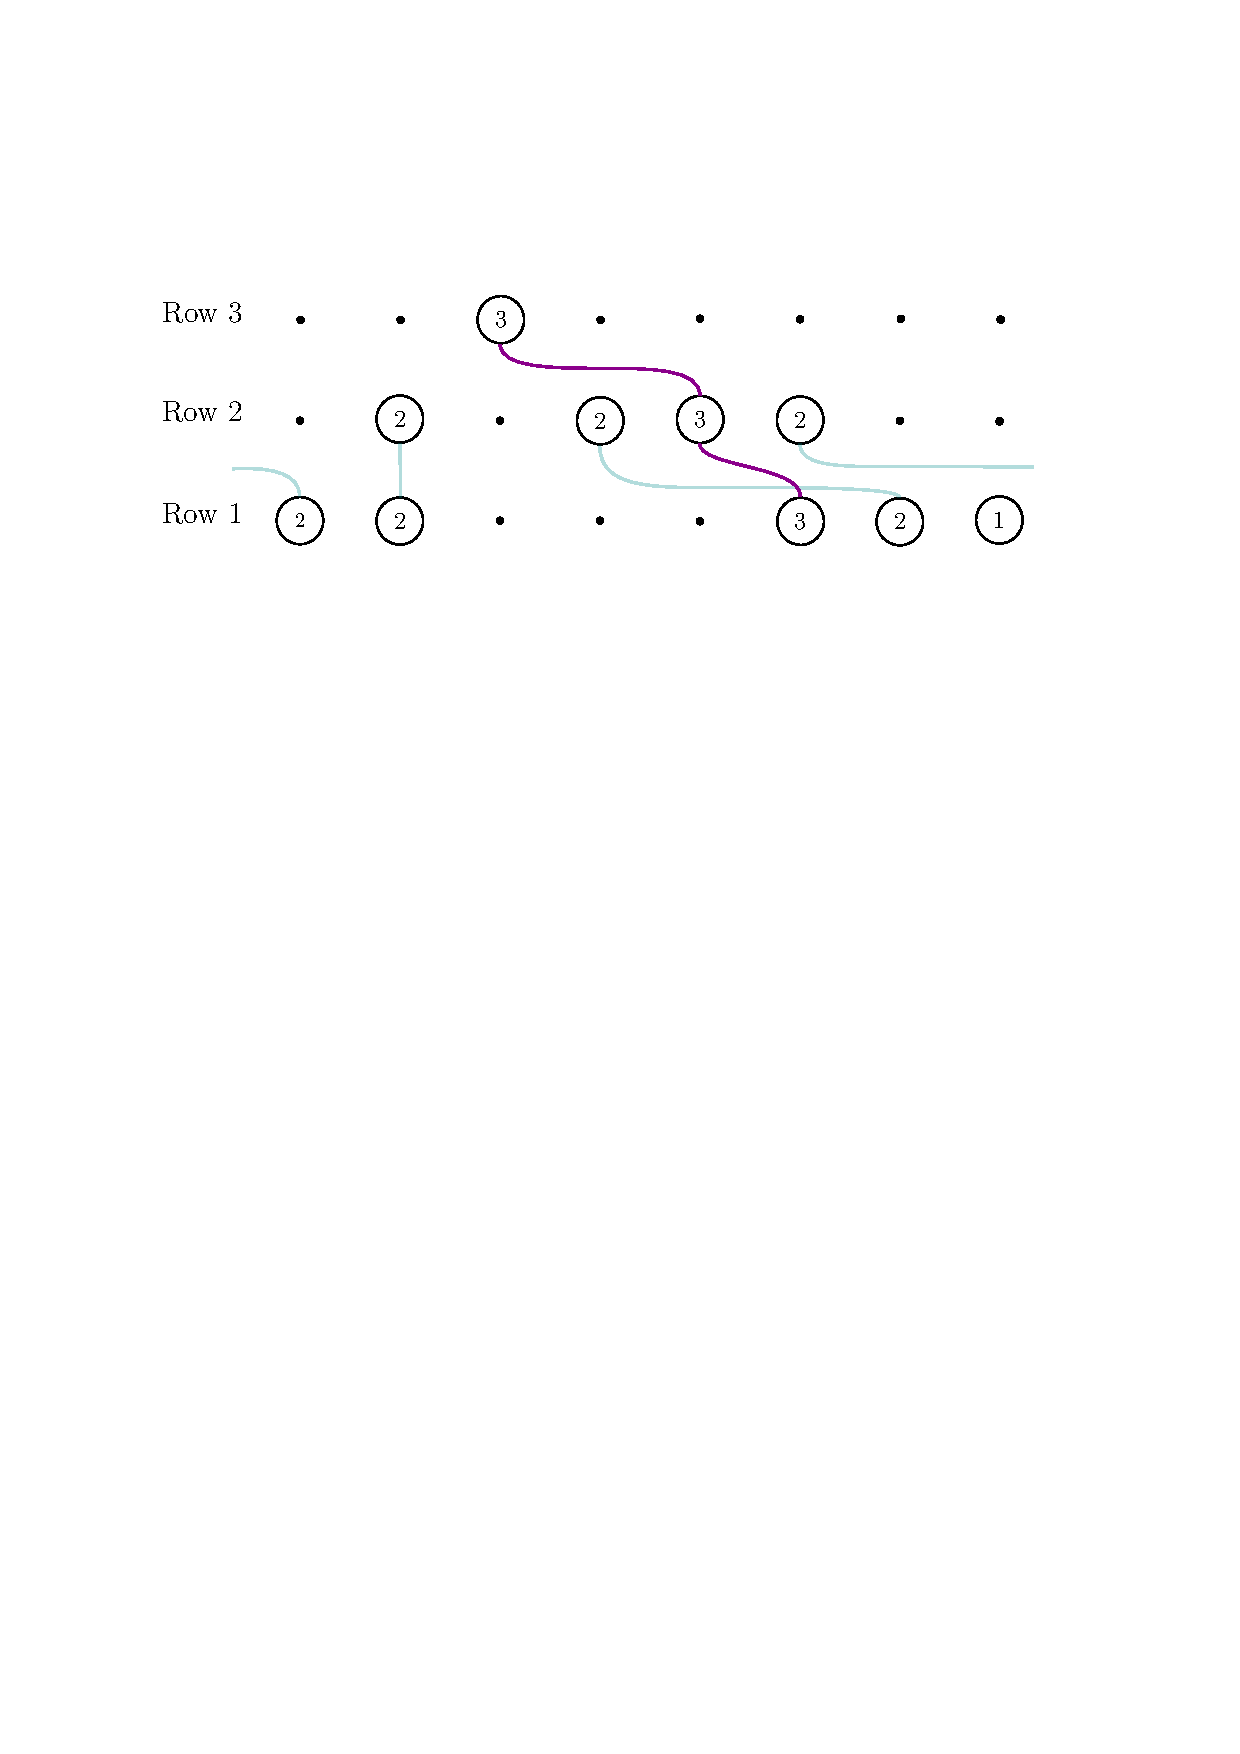
\includegraphics[width=0.5\linewidth]{MLQ2.pdf}
    \caption*{A multiline queue of type $(2,2,0,0,0,3,2,1)$.}
\end{figure}}

\only<4>{\begin{figure}
    \centering
    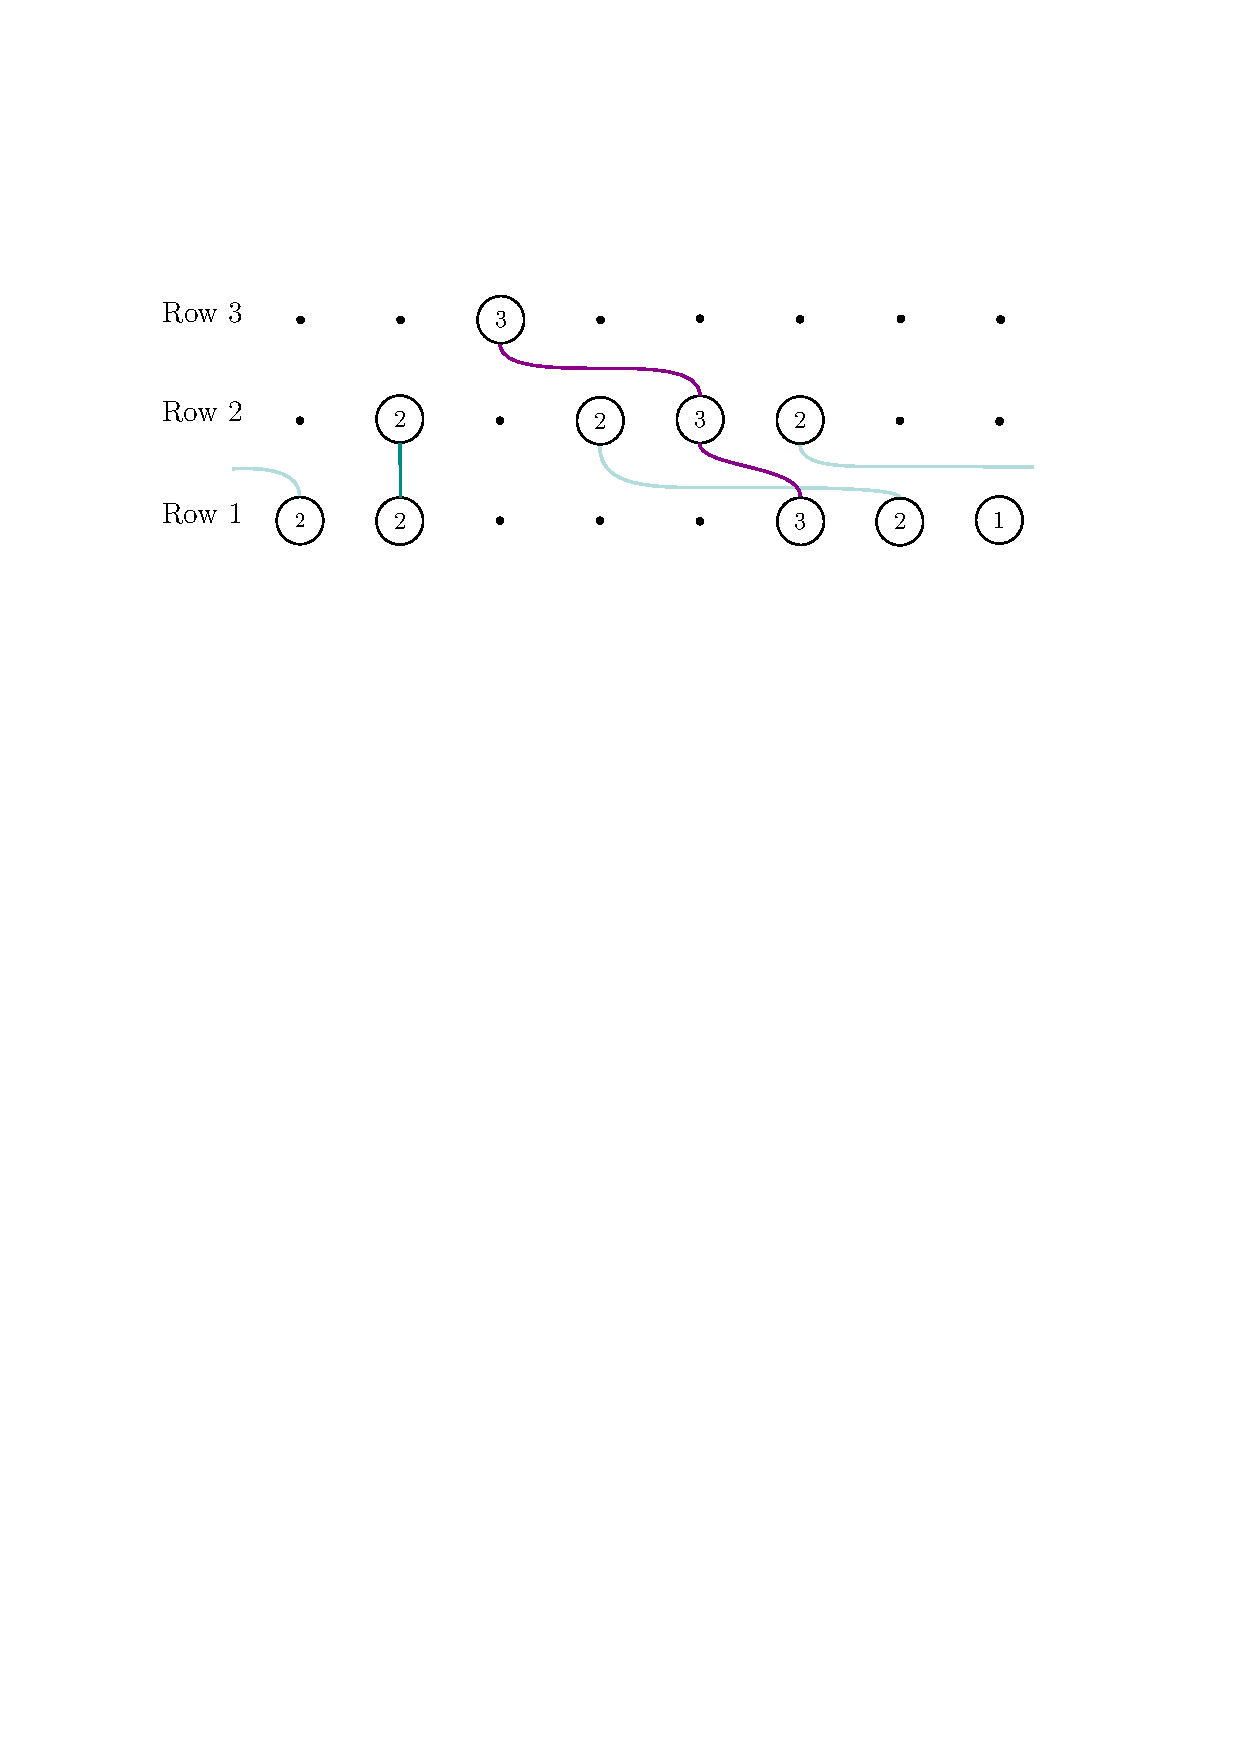
\includegraphics[width=0.5\linewidth]{MLQ3.pdf}
    \caption*{A multiline queue of type $(2,2,0,0,0,3,2,1)$.}
\end{figure}}

\only<5>{\begin{figure}
    \centering
    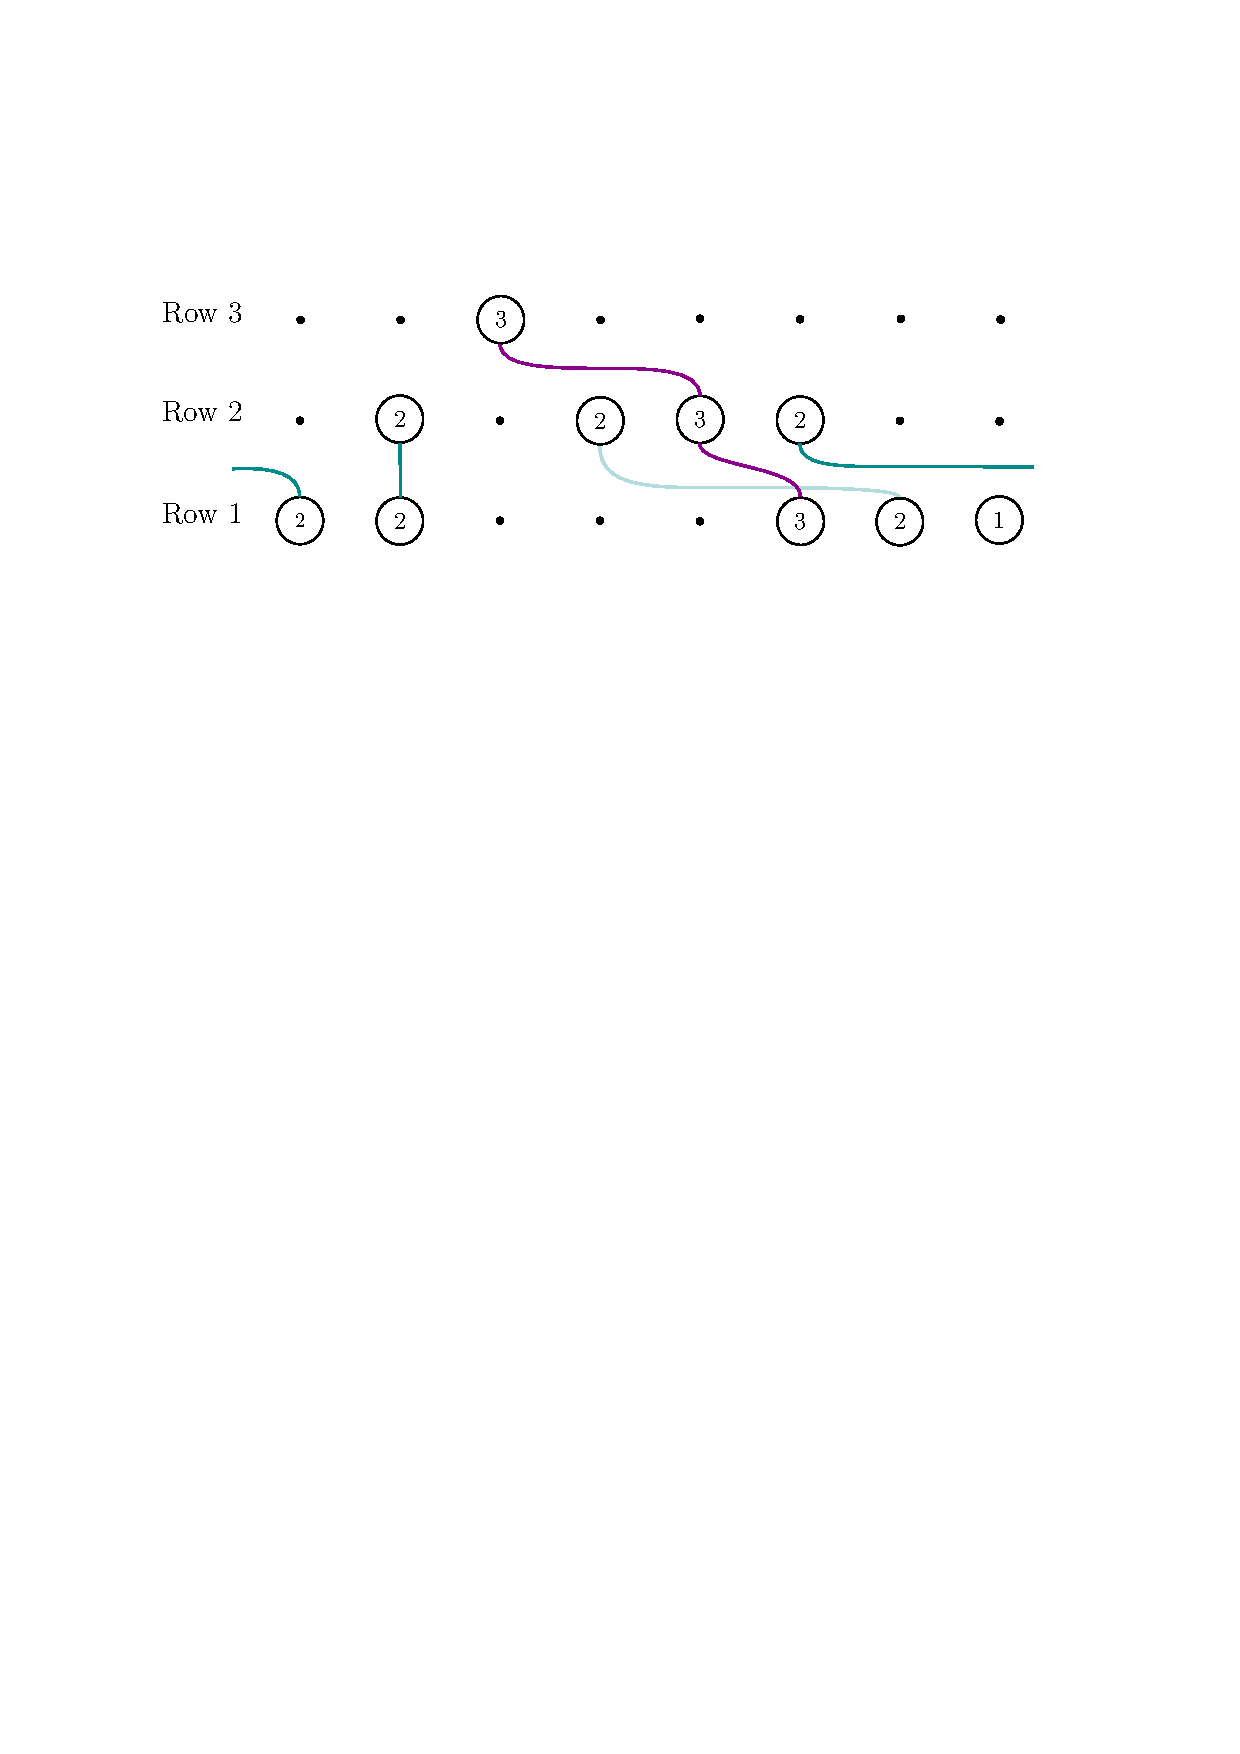
\includegraphics[width=0.5\linewidth]{MLQ4.pdf}
    \caption*{A multiline queue of type $(2,2,0,0,0,3,2,1)$.}
\end{figure}}


\only<6-7>{\begin{figure}
    \centering
    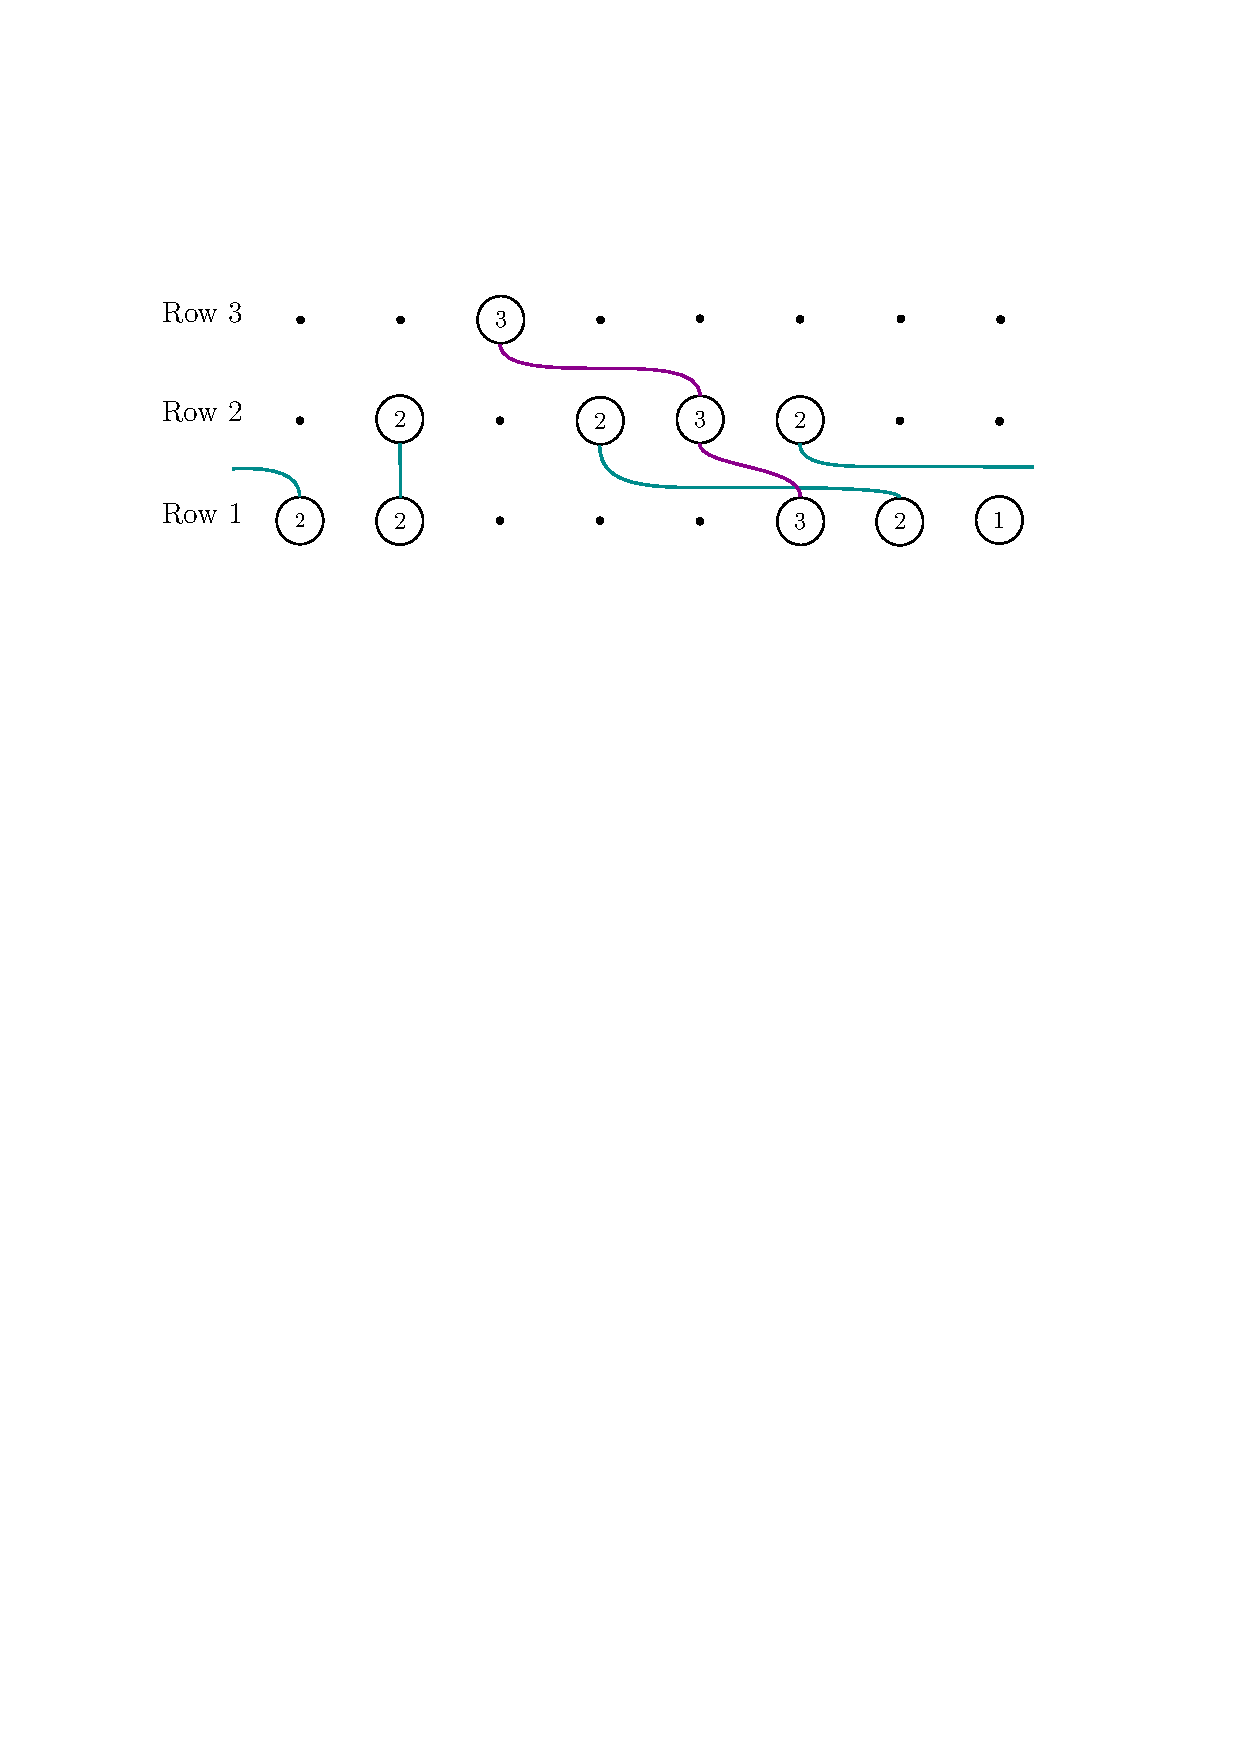
\includegraphics[width=0.5\linewidth]{MLQ5.pdf}
    \caption*{A multiline queue of type $(2,2,0,0,0,3,2,1)$.}
\end{figure}}

\only<1>{
\vspace{-0.6cm}
$$\wt(Q)=x_1 x_2^2 x_3 x_4 x_5 x_6^2 x_7 x_8\semitransp{\frac{(1-t)t}{1-qt^4}\frac{1-t}{1-q^2t^5}\frac{(1-t)qt^2}{1-qt^3}\frac{1-t}{1-qt^2}.}$$
}


\only<2>{
\vspace{-0.6cm}
$$\wt(Q)=x_1 x_2^2 x_3 x_4 x_5 x_6^2 x_7 x_8\frac{(1-t)t}{1-qt^4}\semitransp{\frac{1-t}{1-q^2t^5}\frac{(1-t)qt^2}{1-qt^3}\frac{1-t}{1-qt^2}.}$$
}


\only<3,4>{
\vspace{-0.6cm}
$$\wt(Q)=x_1 x_2^2 x_3 x_4 x_5 x_6^2 x_7 x_8\frac{(1-t)t}{1-qt^4}\frac{1-t}{1-q^2t^5}\semitransp{\frac{(1-t)qt^2}{1-qt^3}\frac{1-t}{1-qt^2}.}$$
}

\only<5>{
\vspace{-0.6cm}
$$\wt(Q)=x_1 x_2^2 x_3 x_4 x_5 x_6^2 x_7 x_8\frac{(1-t)t}{1-qt^4}\frac{1-t}{1-q^2t^5}\frac{(1-t)qt^2}{1-qt^3}\semitransp{\frac{1-t}{1-qt^2}.}$$
}

\only<6>{
\vspace{-0.6cm}
$$\wt(Q)=x_1 x_2^2 x_3 x_4 x_5 x_6^2 x_7 x_8\frac{(1-t)t}{1-qt^4}\frac{1-t}{1-q^2t^5}\frac{(1-t)qt^2}{1-qt^3}\frac{1-t}{1-qt^2}.$$
}

\pause
% We place pairings between row $r>1$ and row $r-1$ in the following order: 
% \vspace{-0.5cm}
% \begin{itemize}
%     \item we place the pairings in decreasing order of their labels,
%     \item within each label, we start by placing the trivial pairings, we then place the other pairings from right to left.
% \end{itemize} 

\end{frame}













\begin{frame}{The multiline queue formula for Macdonald polynomials}
\begin{figure}
    \centering
    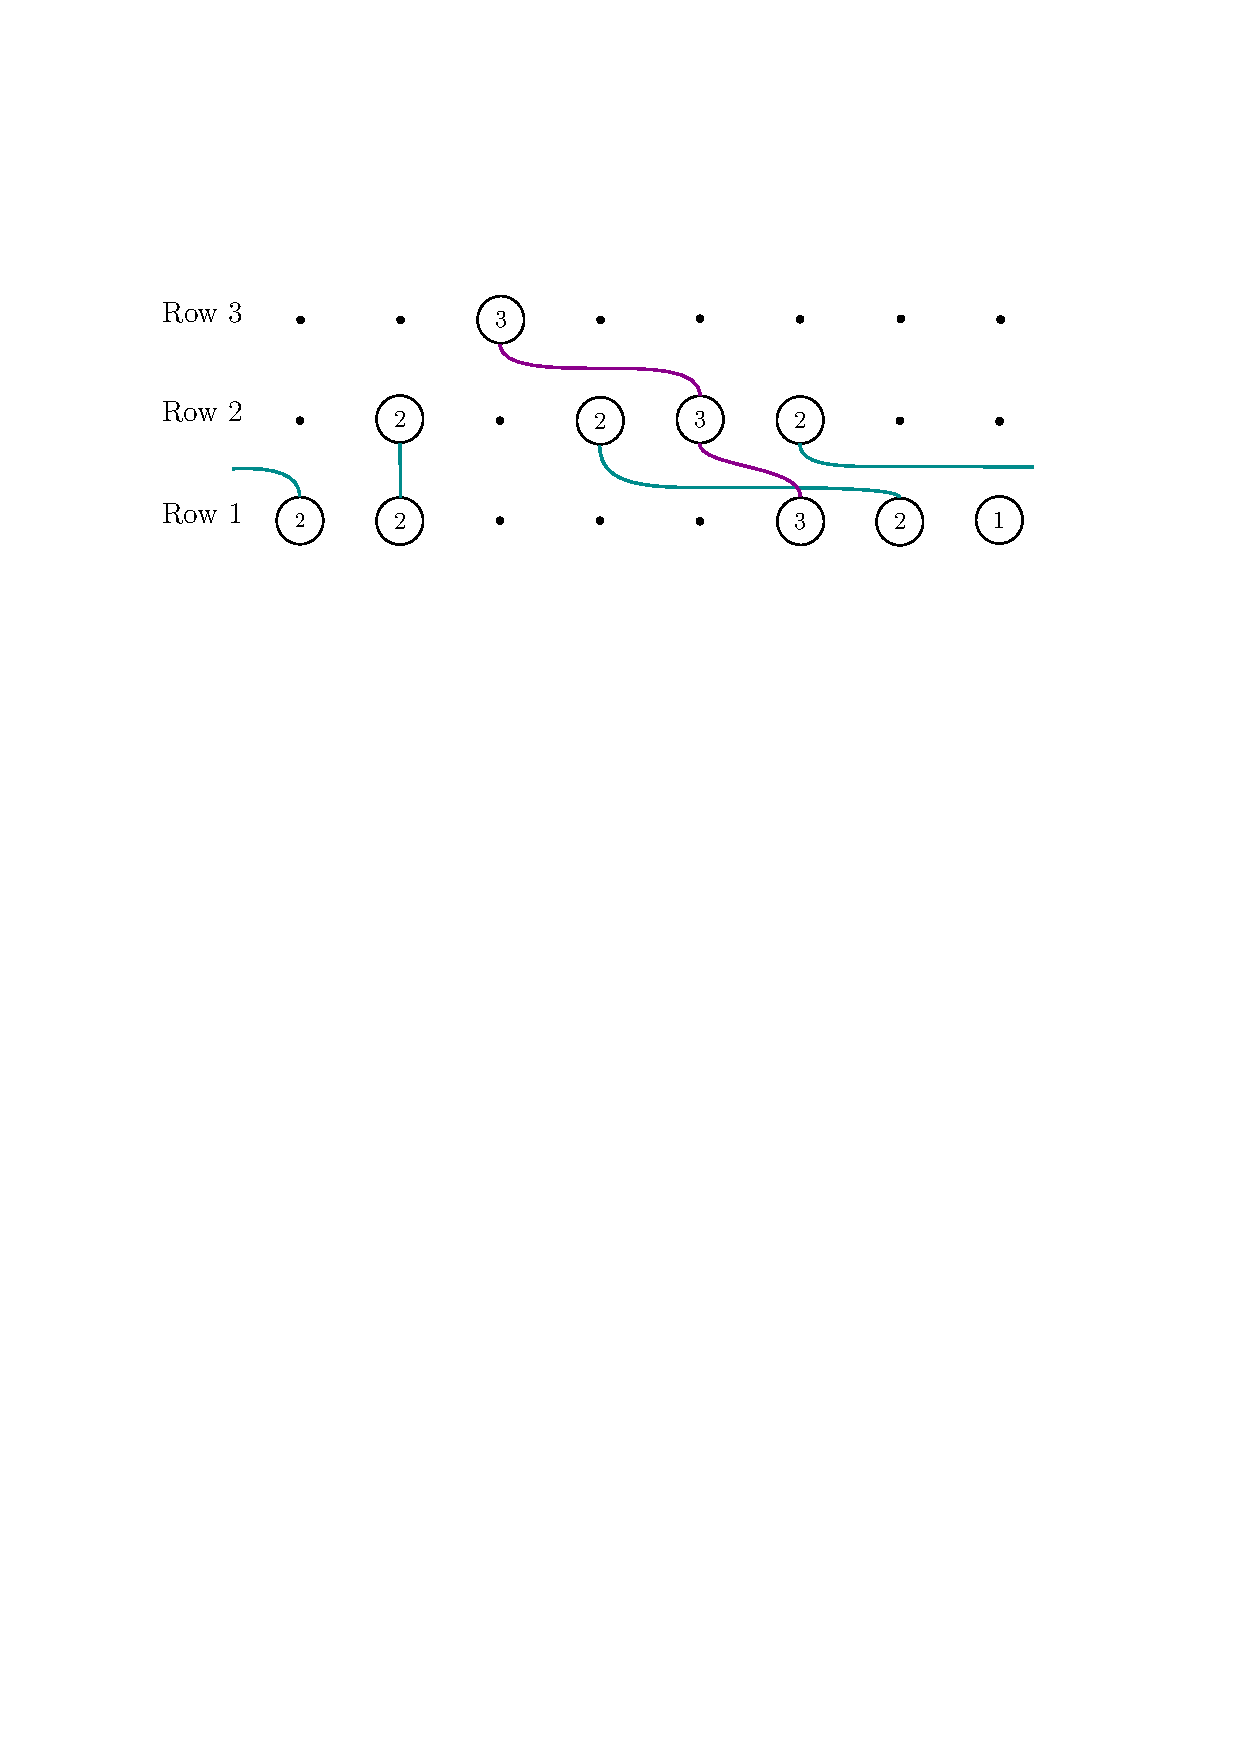
\includegraphics[width=0.45\linewidth]{MLQ5.pdf}
    \caption*{A multiline queue of type $(2,2,0,0,0,3,2,1)$.}
\end{figure}
\vspace{-0.6cm}
$$\wt(Q)=x_1 x_2^2 x_3 x_4 x_5 x_6^2 x_7 x_8\frac{(1-t)t}{1-qt^4}\frac{1-t}{1-q^2t^5}\frac{(1-t)qt^2}{1-qt^3}\frac{1-t}{1-qt^2}.$$
    \begin{thm}[Corteel--Mandelshtam--Williams '23]
For any composition $\mu$, we have
$$f_\mu(x_1,\dots,x_n;q,t)=\sum_{\substack{\text{multiline-queues}\\Q \text{ of type }\mu}}\wt(Q).$$
\vspace{-0.3cm}
As a consequence, for any partition $\lambda$,
$$P_\lambda(x_1,\dots,x_n;q,t)=\sum_{\mu\in S_n(\lambda)}\ \sum_{\substack{\text{multiline-queues}\\Q \text{ of type }\mu}}\wt(Q).$$
\end{thm}

\end{frame}














\begin{frame}{Signed Multiline queues}\smaller 
\only<-4>{
\textcolor{uibred}{An enhanced ball system} 
is a $2L \times n$ array ($L,n\geq 1$), with rows labeled from bottom to top as $1, 1', 2, 2', \dots, L,L'$,
and columns labeled from left to right from $1$ to $n$,
in which each of the $2Ln$ positions is either empty or occupied by a ball. A ball in row $r$ is labeled by $a>0$, and a ball in row $r'$ is labeled $\pm a$, where $a>0$.
\vspace{-0.3cm}}

 A \textcolor{uibred}{signed multiline queue} is an enhanced ball system, satisfying the conditions:
 \only<-4>{
 \vspace{-0.4cm}
\begin{itemize}
    \item each pair connects two balls with the same absolute value,
    \item after forgetting the signs, classic layers correspond to layers from classic MLQ.
\item each ball in row $r'$ is paired with a ball in row $r$, using the shortest strand traveling (weakly) from left to right, \textcolor{uibred}{without wrapping around}.
     \item it does not contain any forbidden configuration.
\end{itemize}}
\only<5>{
 \vspace{-0.4cm}
\begin{itemize}
     \item it does not contain any forbidden configuration.
\end{itemize}}
\vspace{-0.4cm}
\only<-2,5>{
\begin{figure}
    \centering
    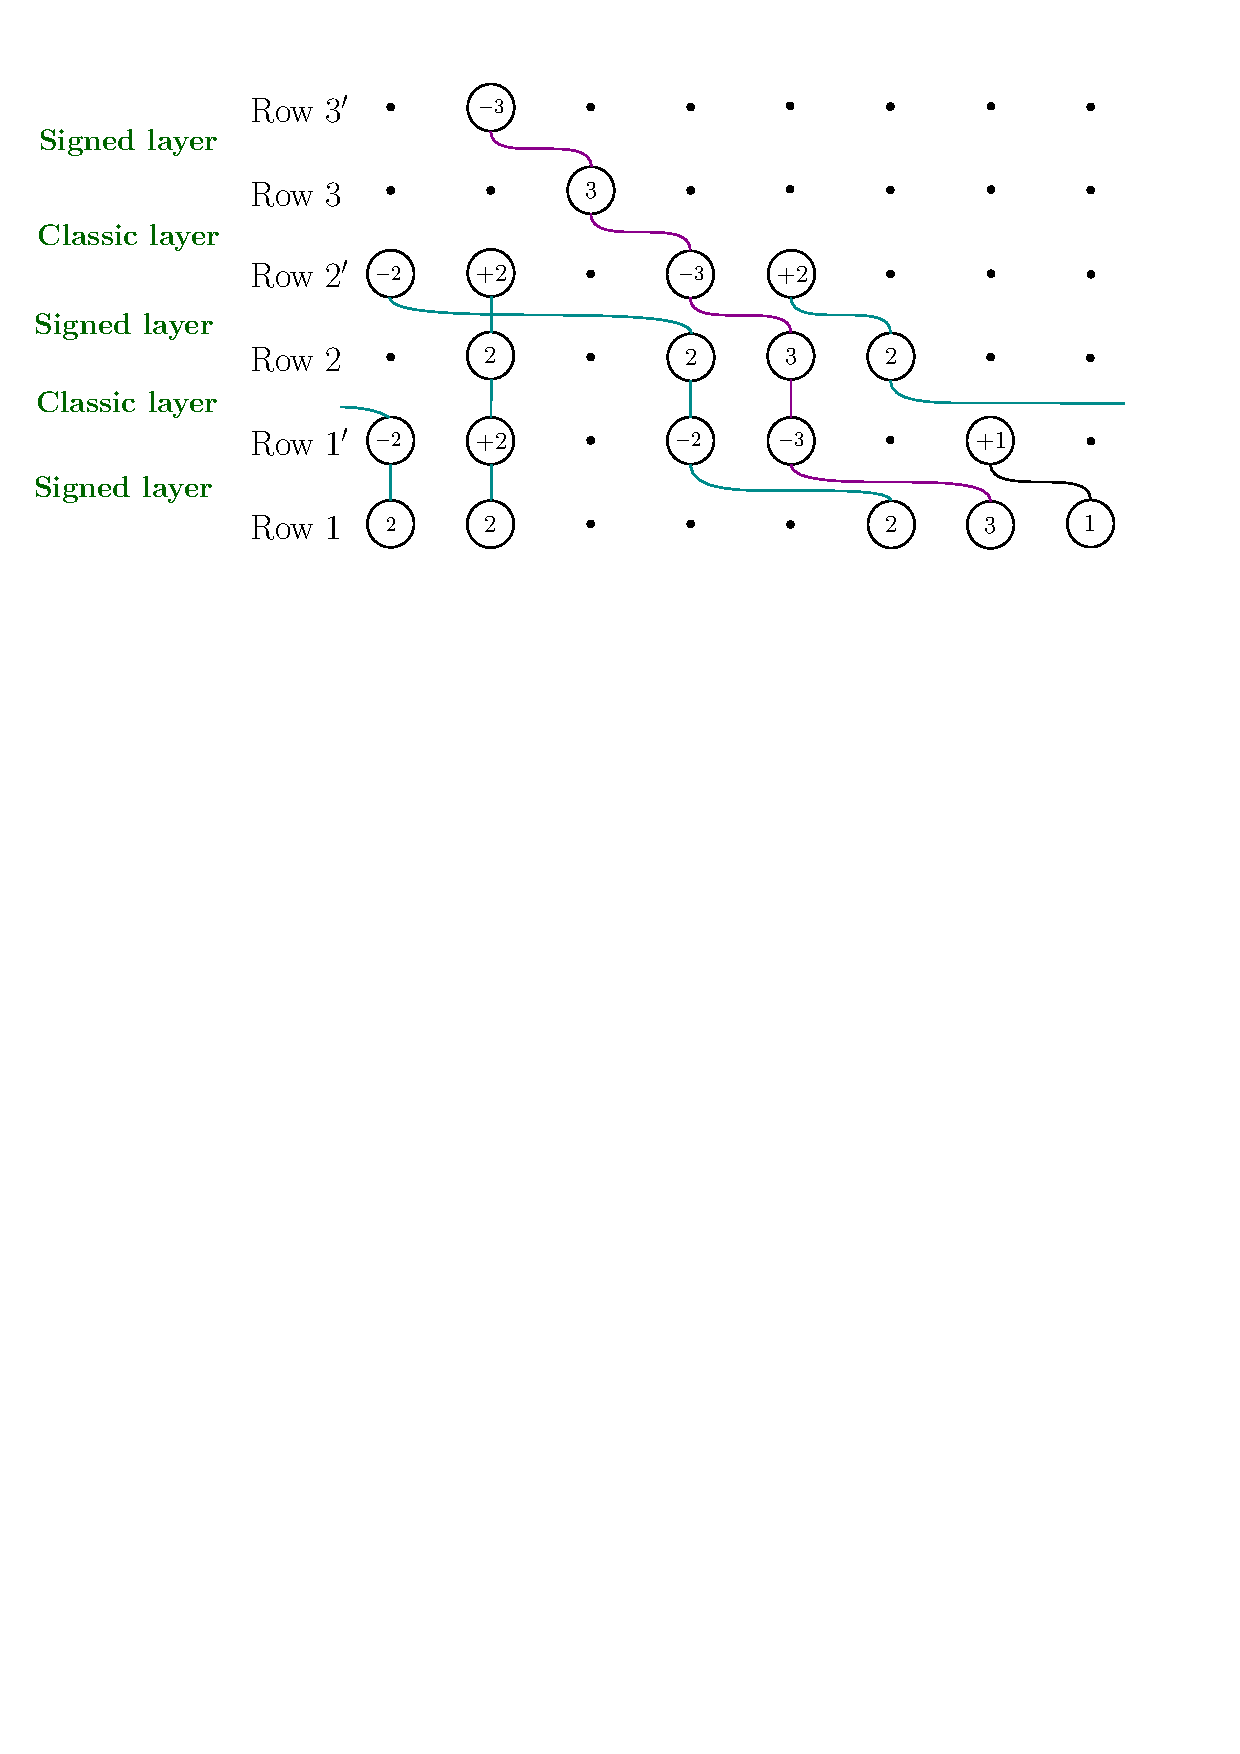
\includegraphics[width=0.6\linewidth]{GhostMLQ.pdf}
    \caption*{A signed multiline queue of type $(2,2,0,0,0,3,2,1)$.}
\end{figure}}

\only<3>{
\begin{figure}
    \centering
    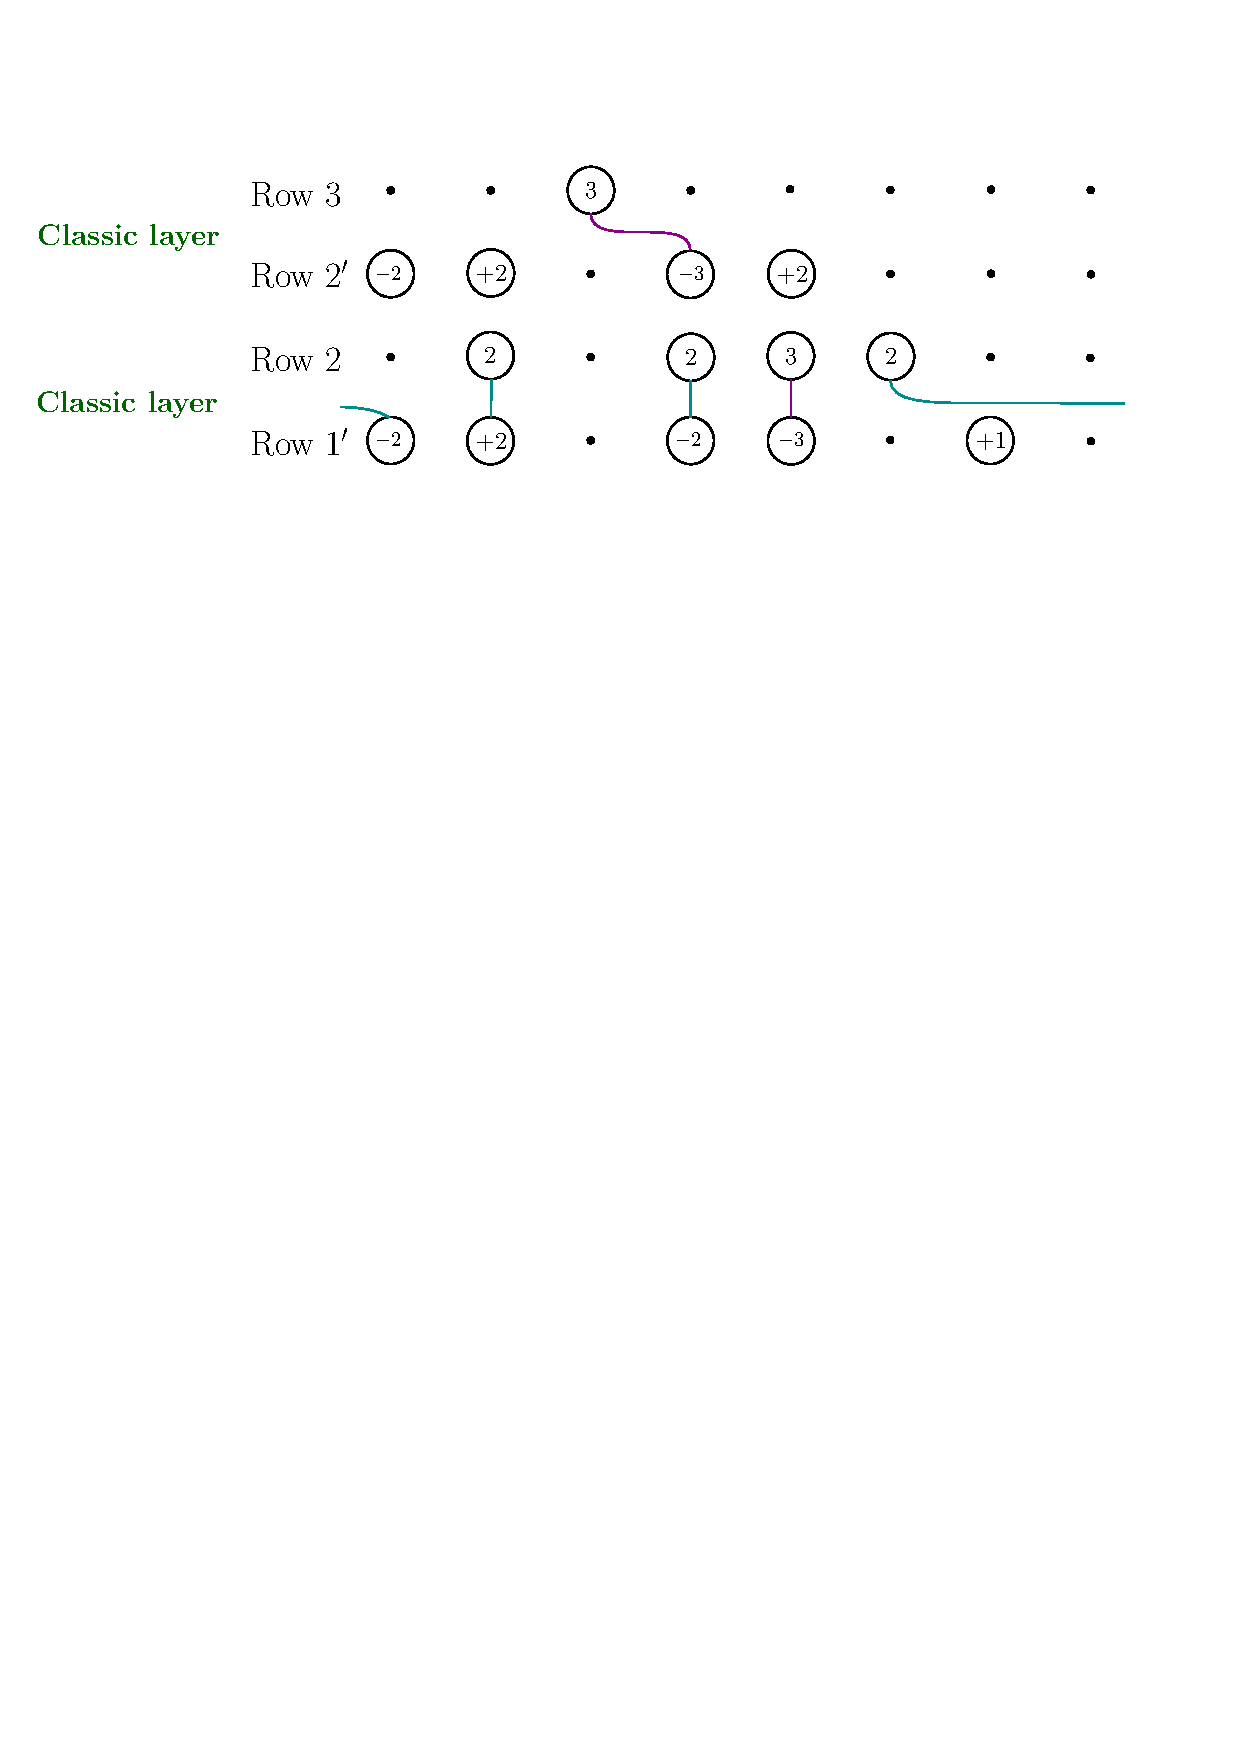
\includegraphics[width=0.6\linewidth]{Classic layers.pdf}
    \caption*{Classic layers of a signed multiline queue.}
\end{figure}}

\only<4>{
\begin{figure}
    \centering
    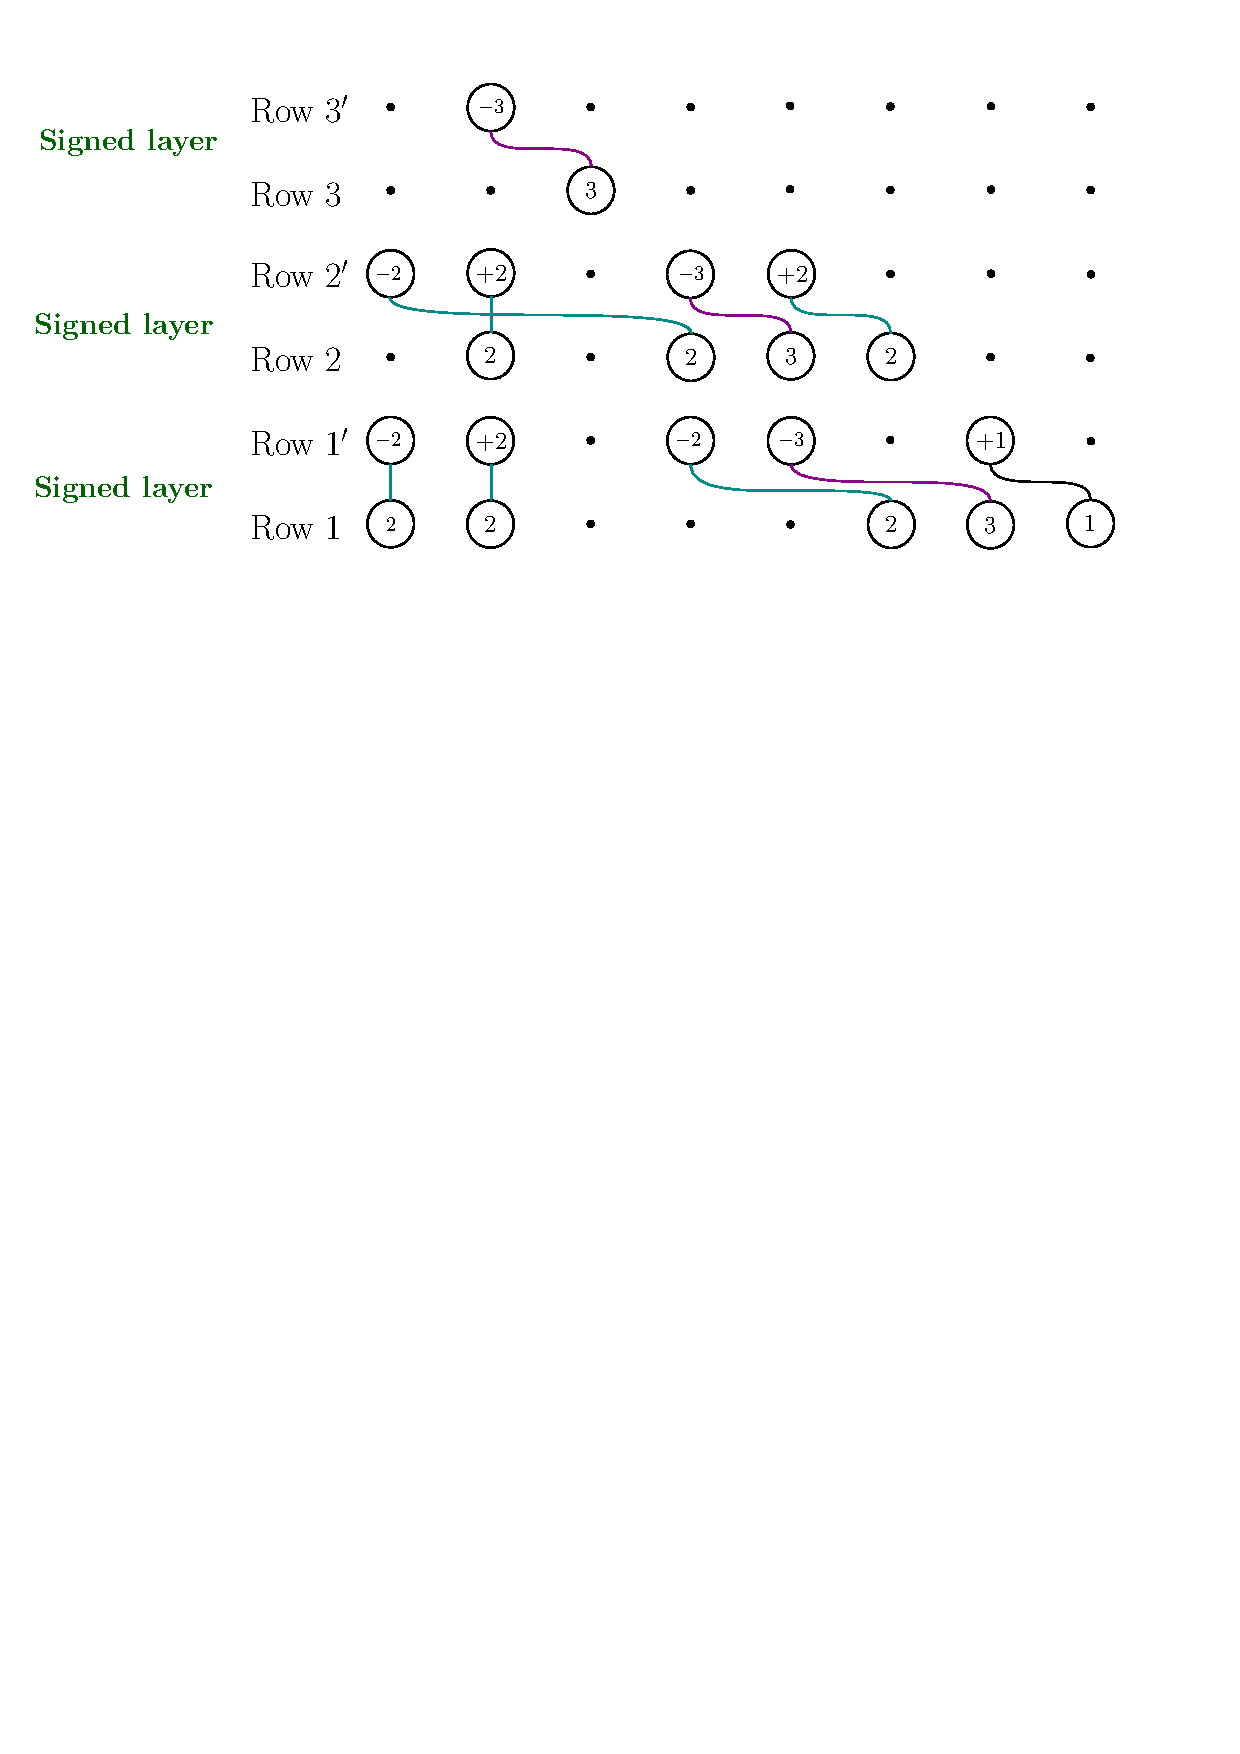
\includegraphics[width=0.6\linewidth]{Signed layers.pdf}
    \caption*{Signed layers of a signed multiline queue.}
\end{figure}}


\only<5>{
\vspace{-0.63cm}
\begin{figure}
    \centering
    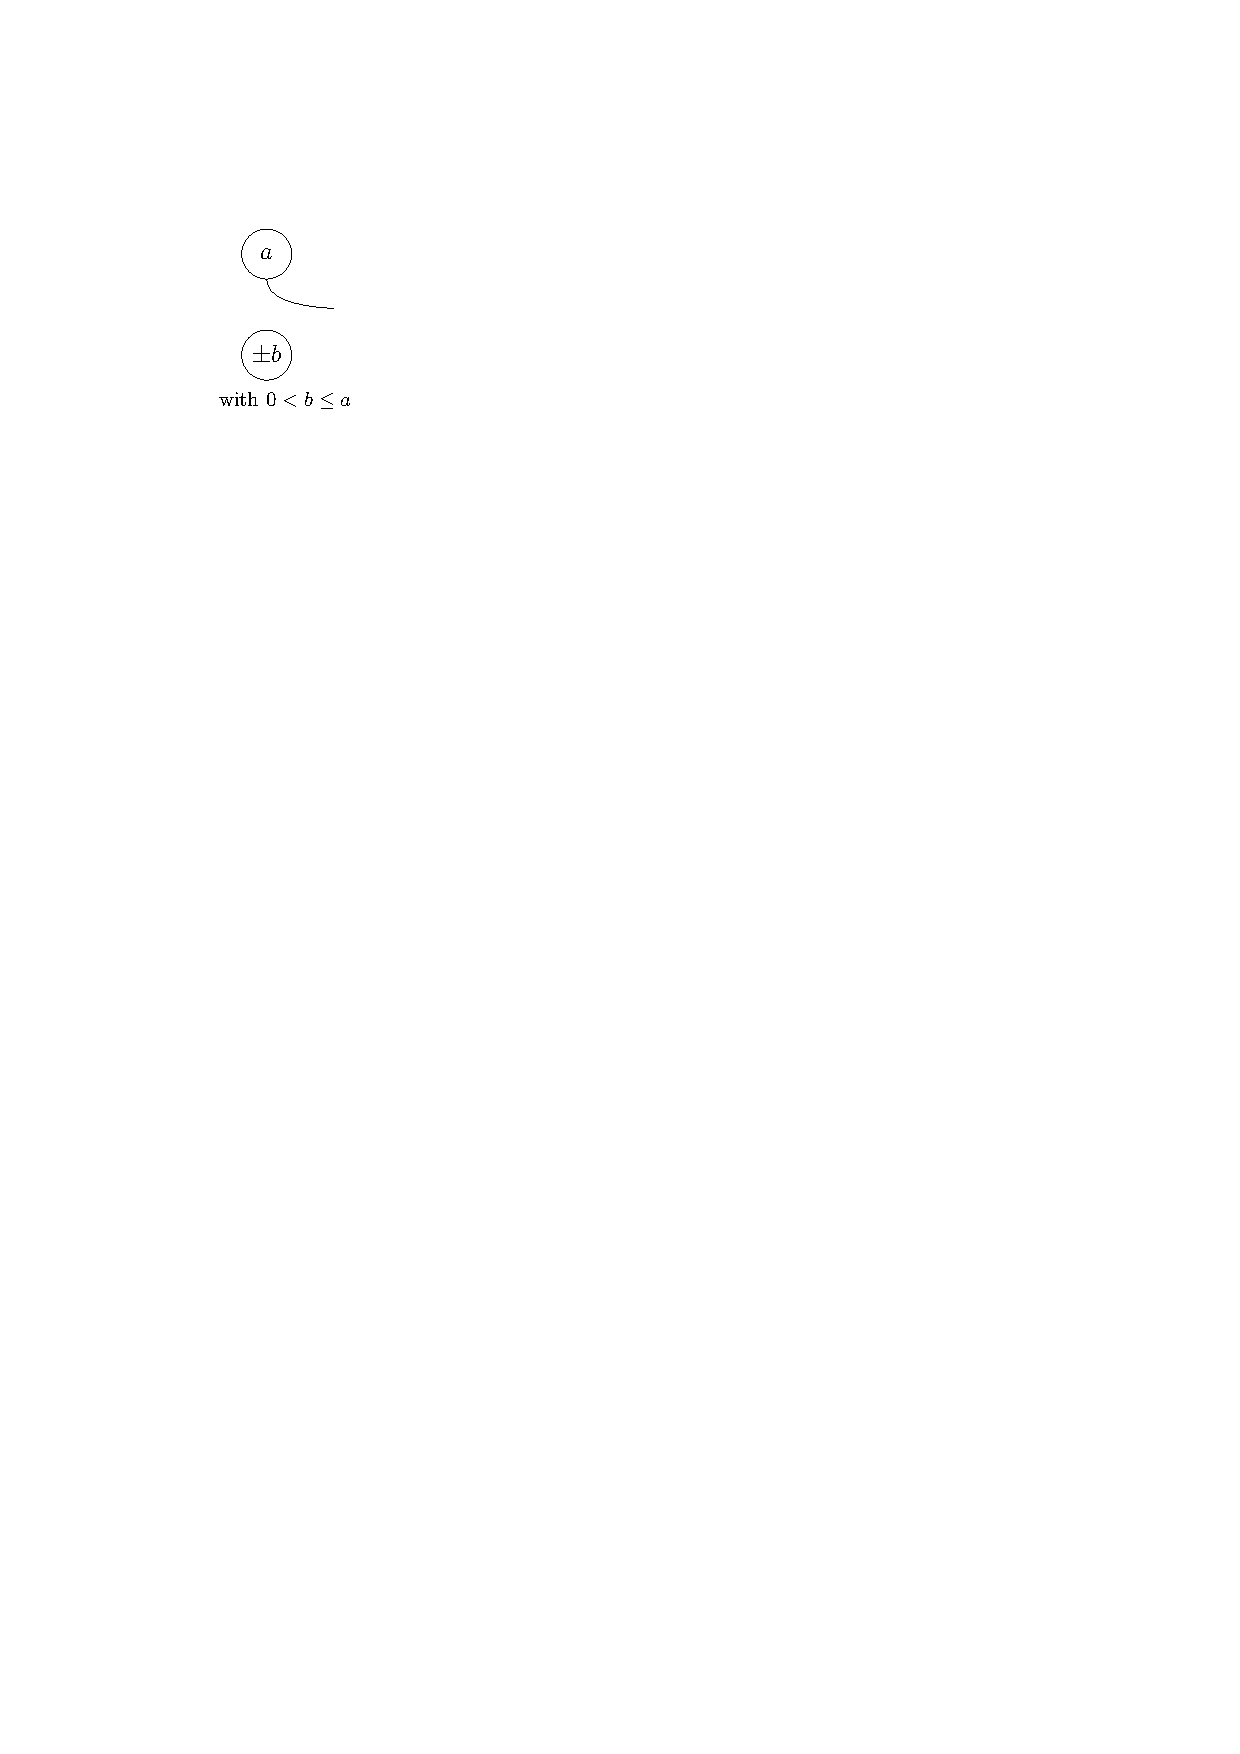
\includegraphics[height=0.15\linewidth]{Forbidden configuration classic.pdf}
    \hspace{1cm}
    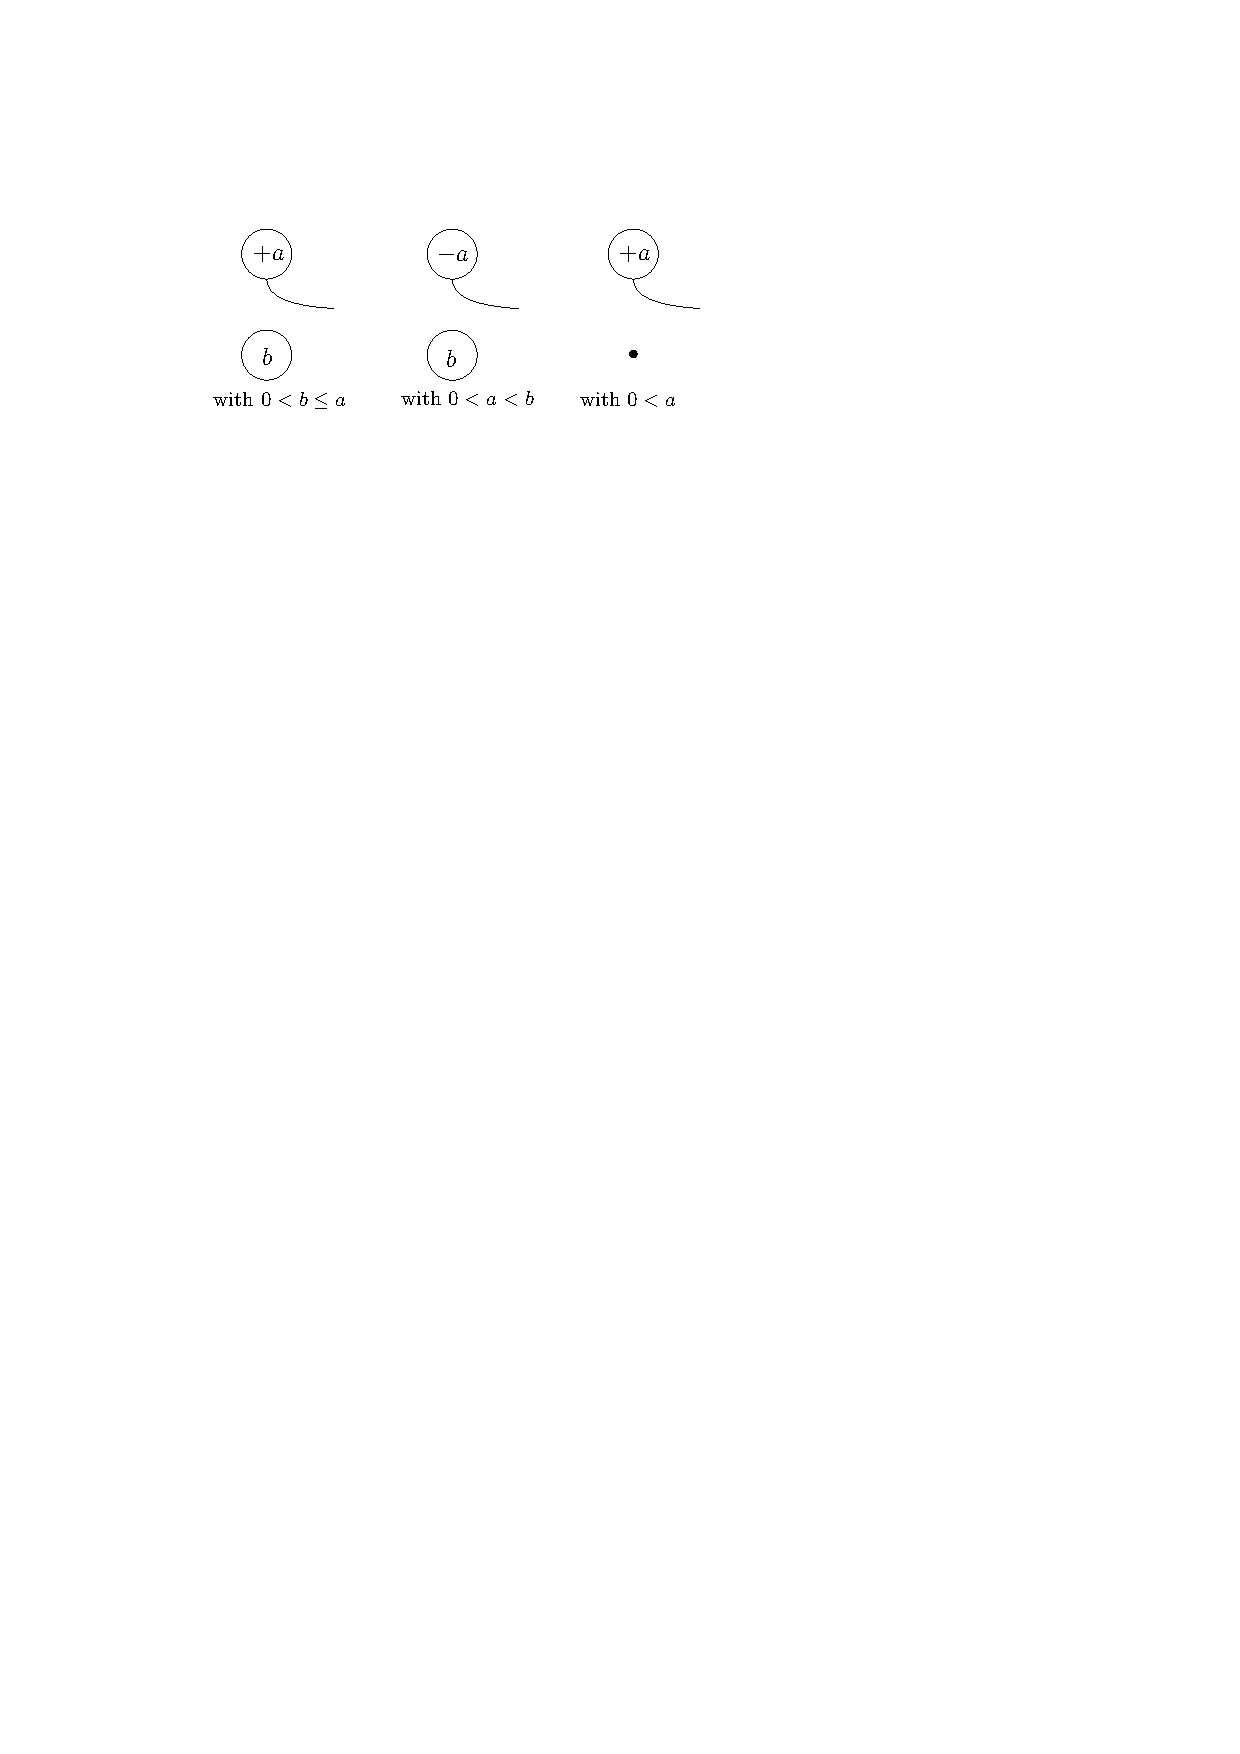
\includegraphics[height=0.15\linewidth]{Forbidden configurations ghost.pdf}    
    \caption*{The forbidden configuration for signed multiline queues.}
\end{figure}   
}



\end{frame}






\begin{frame}{Weights of Signed Multiline Queues}

\begin{itemize}
    \item Only signed balls have weights. A ball in column $i$, row $r'$, has the weight 
    \vspace{-0.3cm}
    $$\begin{cases}
        x_i &\text{if it is positive,}\\
        \frac{-q^{r-1}}{t^{n-1}} &\text{if it is negative.}
    \end{cases}$$
    \item  Each nontrivial pairing $p$ has a weight $\wt_{\textup{pair}(p)}$ (we use the same order to place pairings)
    % \item<2-> pairings in signed layers have the weights.
    % \item The total weight of a multiline queue $Q$ is denoted $\wt(Q)$.
\end{itemize}
\only<1-2>{
\vspace{-0.5cm}

\begin{figure}
    \centering
    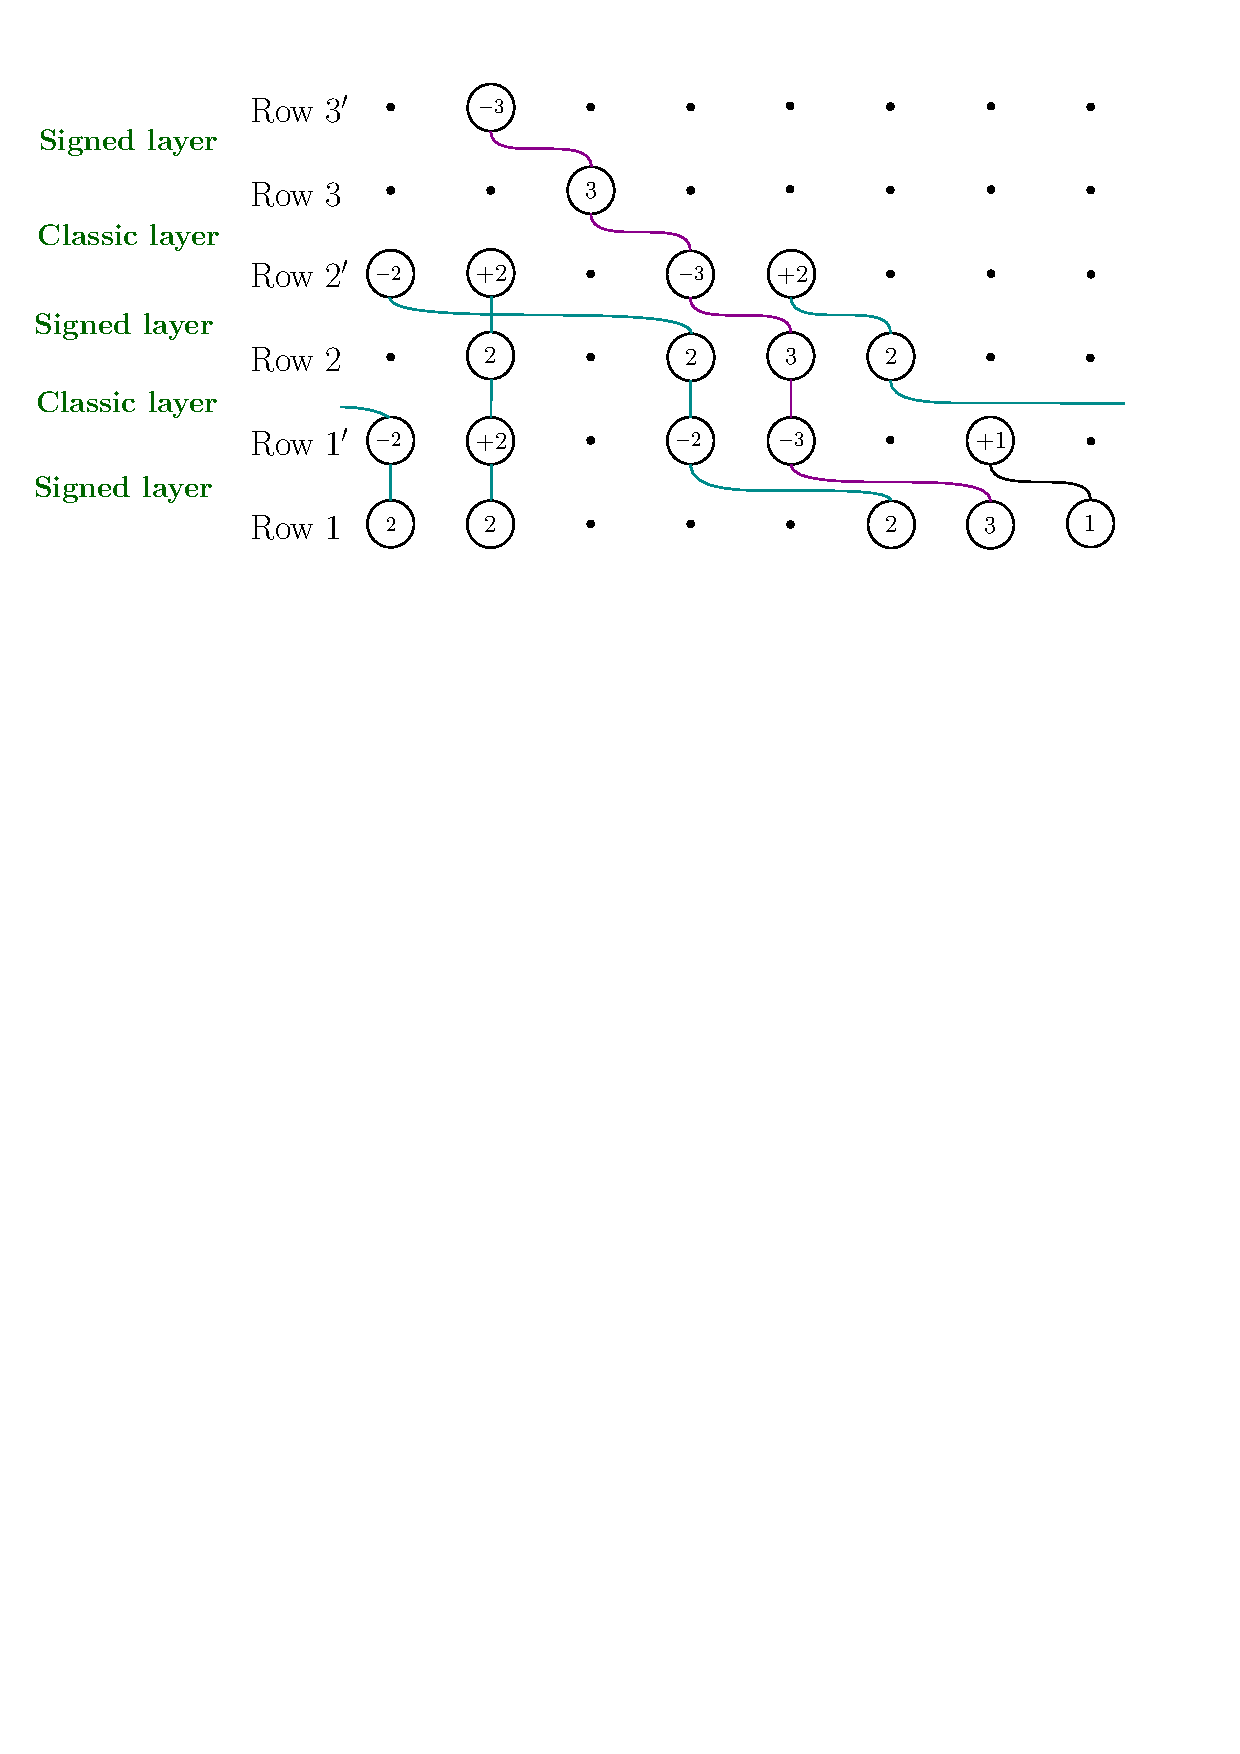
\includegraphics[width=0.64\linewidth]{GhostMLQ.pdf}
    % \caption*{A multiline queue of type $(2,2,0,0,0,3,2,1)$.}
\end{figure}
}

% \only<4->{
% \vspace{-0.5cm}
% \begin{figure}
%     \centering
%     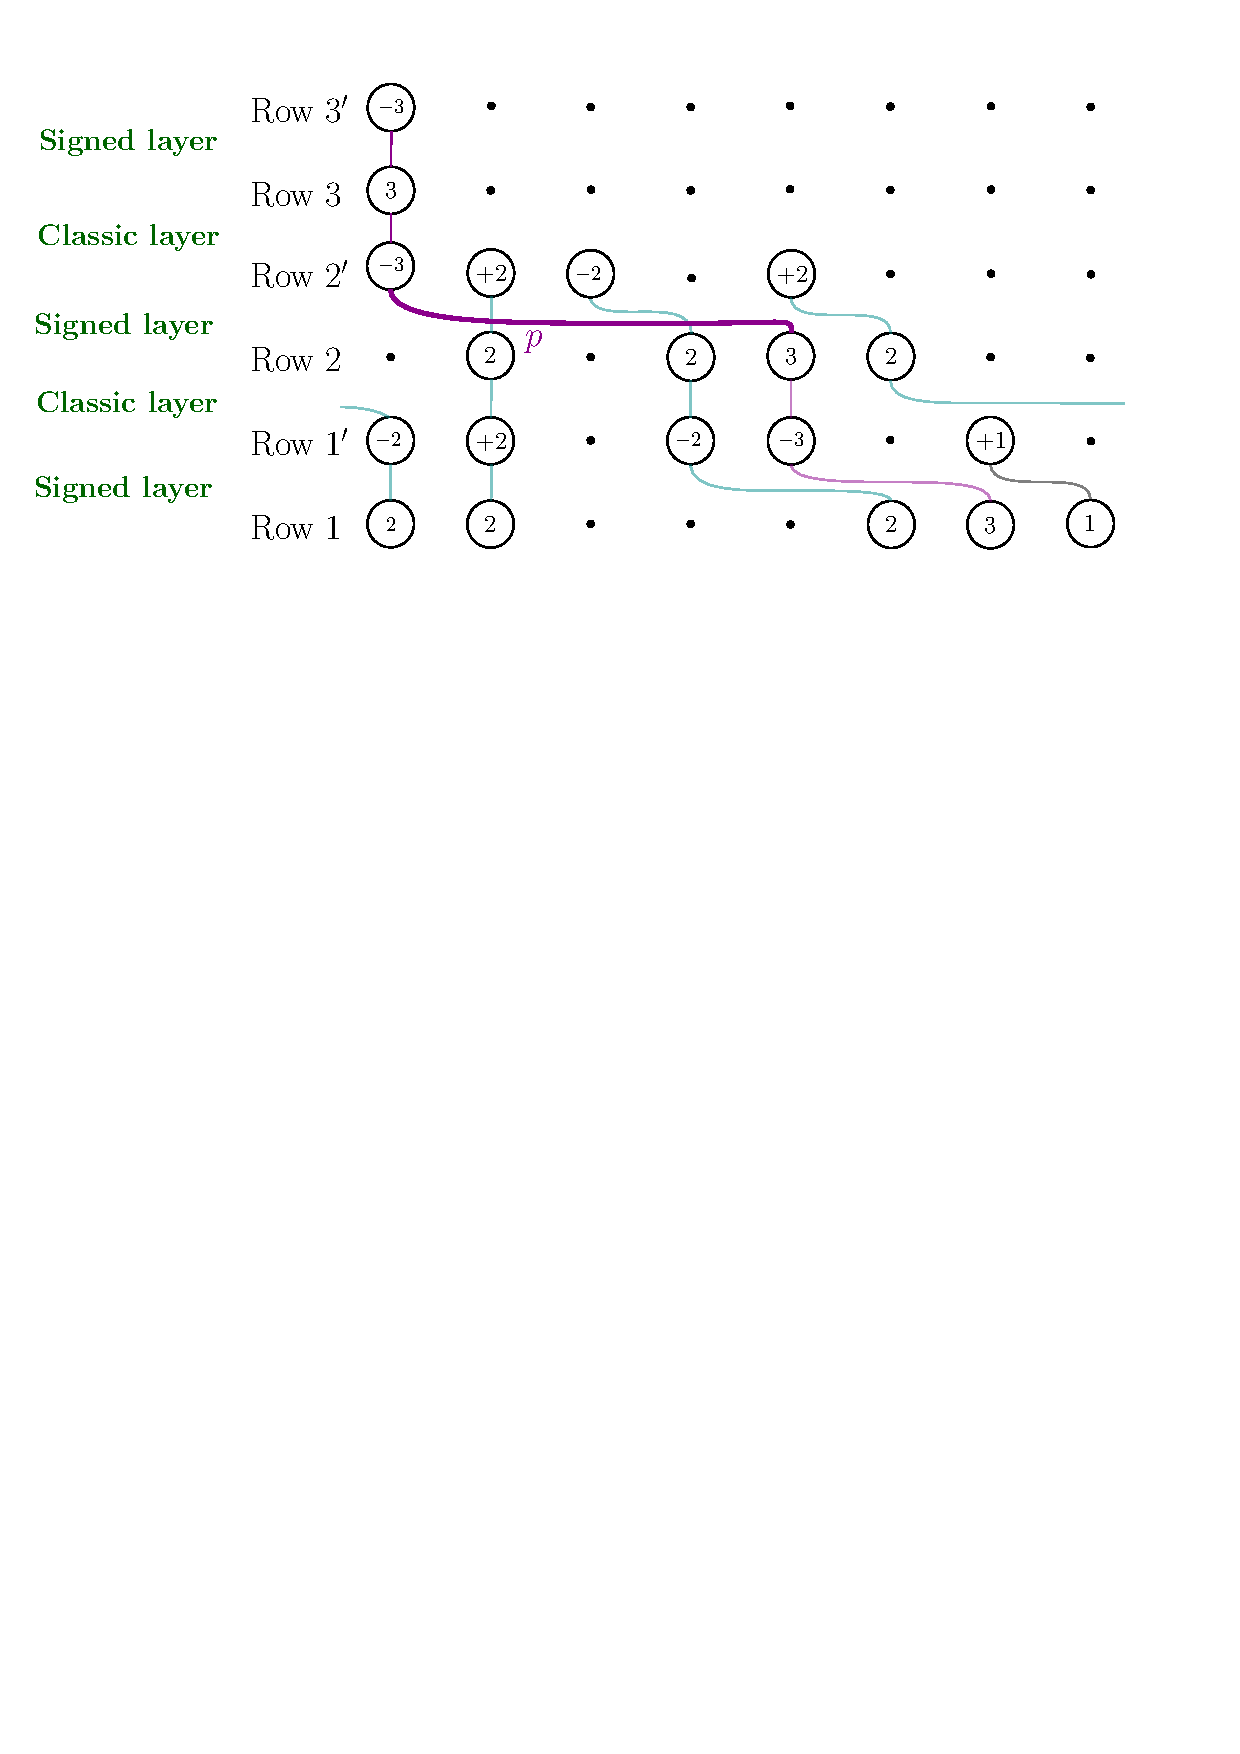
\includegraphics[width=0.57\linewidth]{GhostMLQ2.pdf}
%     % \caption*{A multiline queue of type $(2,2,0,0,0,3,2,1)$.}
% \end{figure}
% \vspace{-0.3cm}
% }

\only<2>{\vspace{-0.6cm}
$$\text{A signed multiline queue with ball weight:} \quad x_2^2x_5x_7\left(\frac{-1}{t^7}\right)^3\left(\frac{-q}{t^7}\right)^2\left(\frac{-q^2}{t^7}\right)$$
}
\vspace{-0.3cm}
\only<3->{
\begin{itemize}
    \item Weights of pairings in classic layers are defined as before,
    \item weight of a nontrivial pairing in  a signed layer is given by
    \begin{equation*}
\hspace{-0.5cm}\wt_{\textup{pair}}(p) = \begin{cases}
         (1-t) t^{\textup{skip}(p)+\textup{empty}(p)} &\text{\smaller if $p$ connects a positive ball and a regular ball}\\
         -(1-t) t^{\textup{skip}(p)+\textup{empty}(p)} &\text{\smaller if $p$ connects a negative ball and a regular ball.}
\end{cases}
\end{equation*}
\end{itemize}}

\only<3>{
\begin{figure}
    \centering
    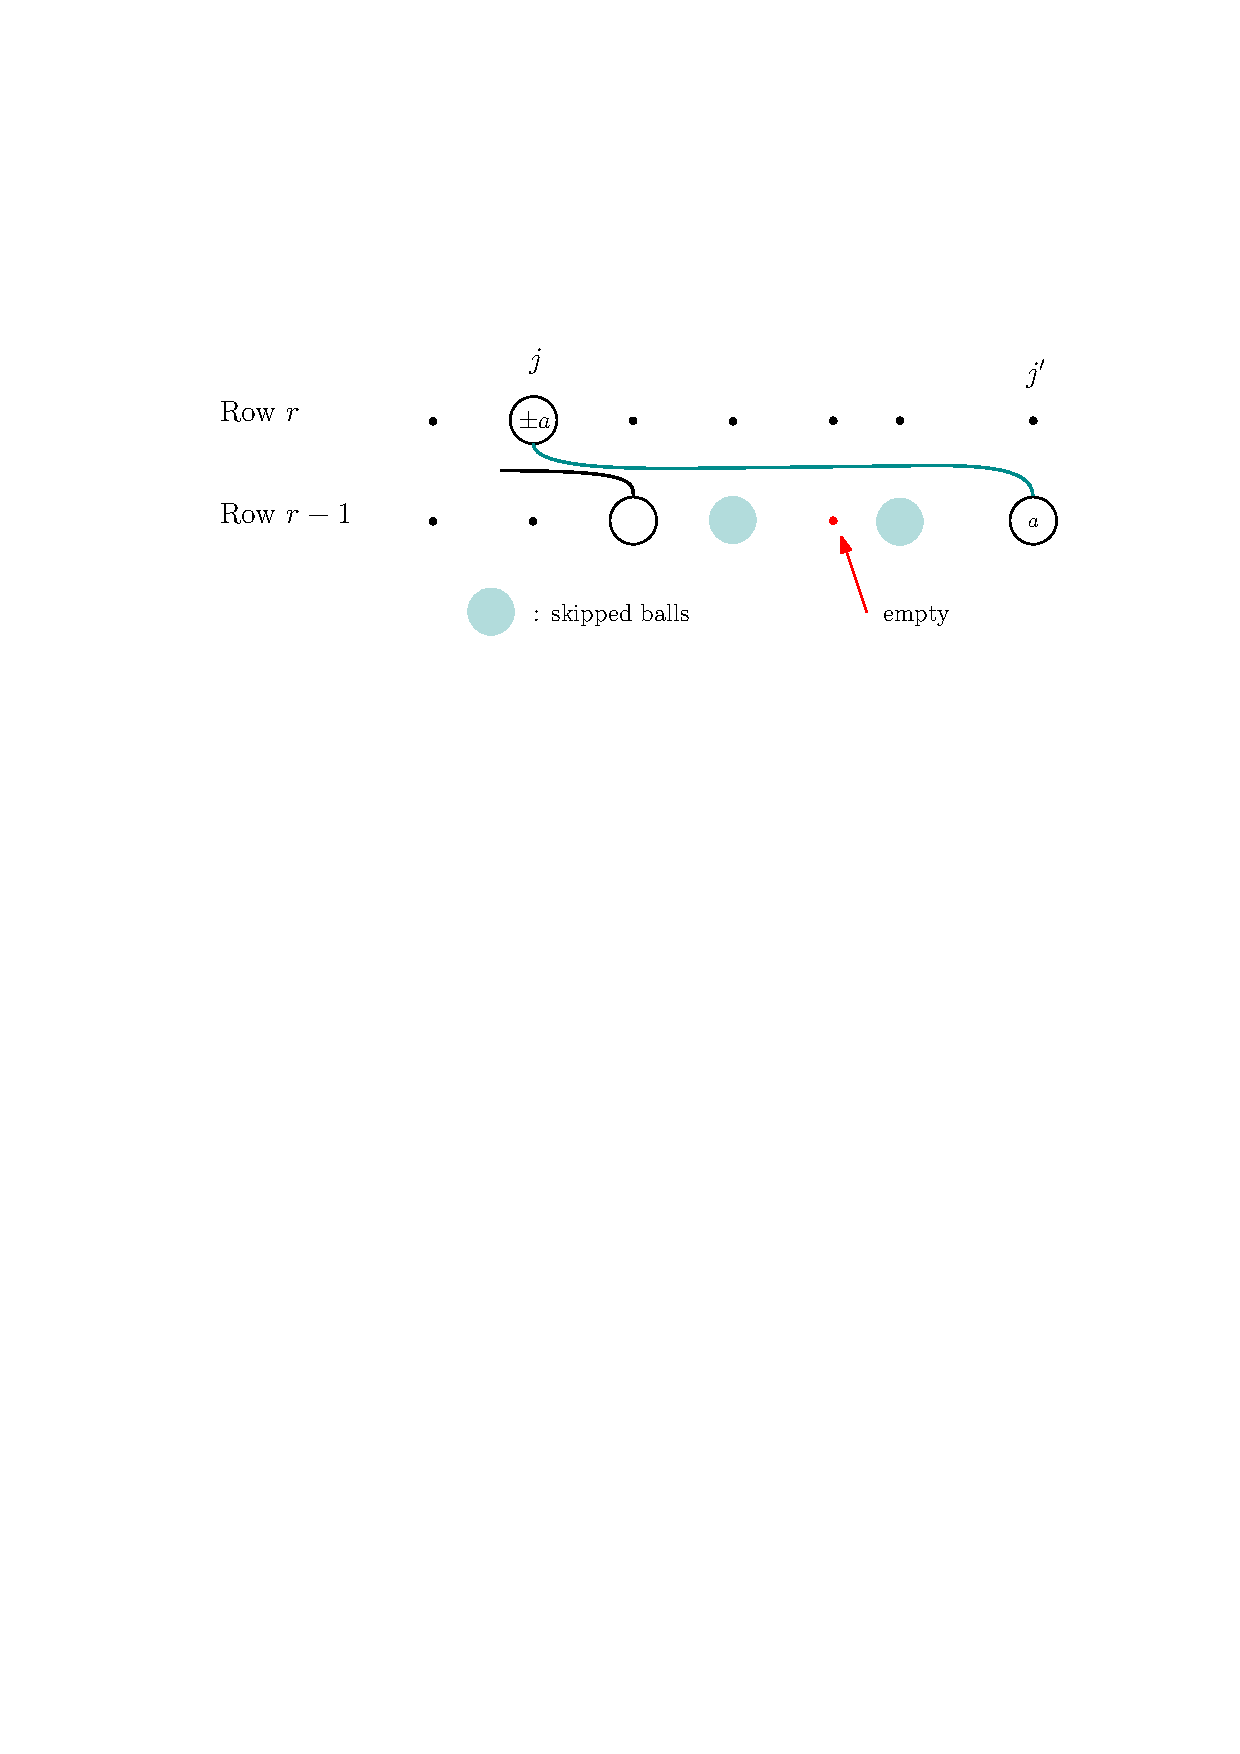
\includegraphics[width=0.9\linewidth]{Signed Pairings.pdf}
    % \caption*{A multiline queue of type $(2,2,0,0,0,3,2,1)$.}
\end{figure}}



% \only<4>{
% \vspace{-0.25cm}
% \textbf{Example: }$\textup{skip}(p)=2$ and $\textup{empty}(p)=1$ $\longrightarrow \wt_{\textup{pair}}(p)=-(1-t)t^3.$}





\end{frame}





\begin{frame}{Signed Multiline queues}

 \textbf{\textcolor{uibred}{Remark:}} In the homogeneous part, all signed balls should be positive.
 
 A signed multiline queue without negative balls is a multiline queue.

    $$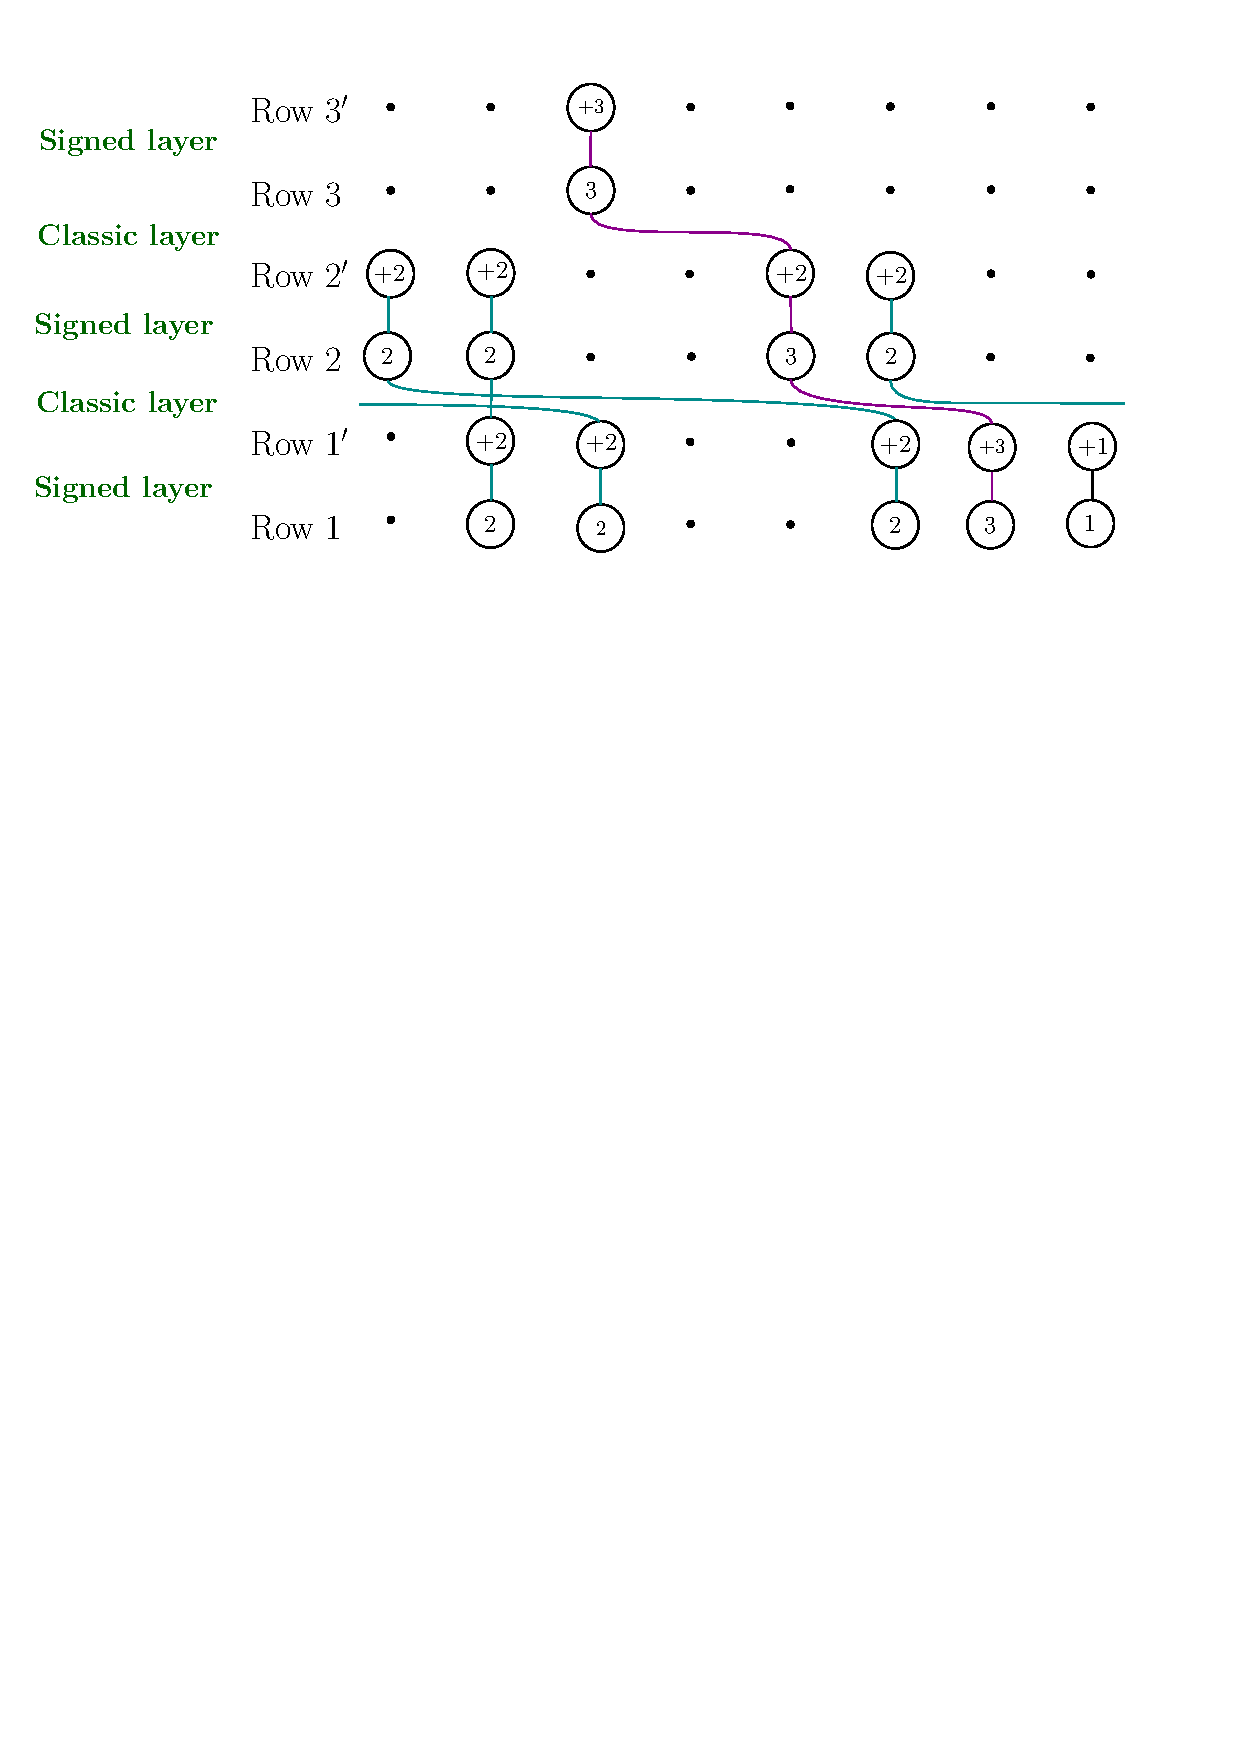
\includegraphics[height=0.19\linewidth,valign=c]{GhostMLQtr.pdf}
    \equiv
    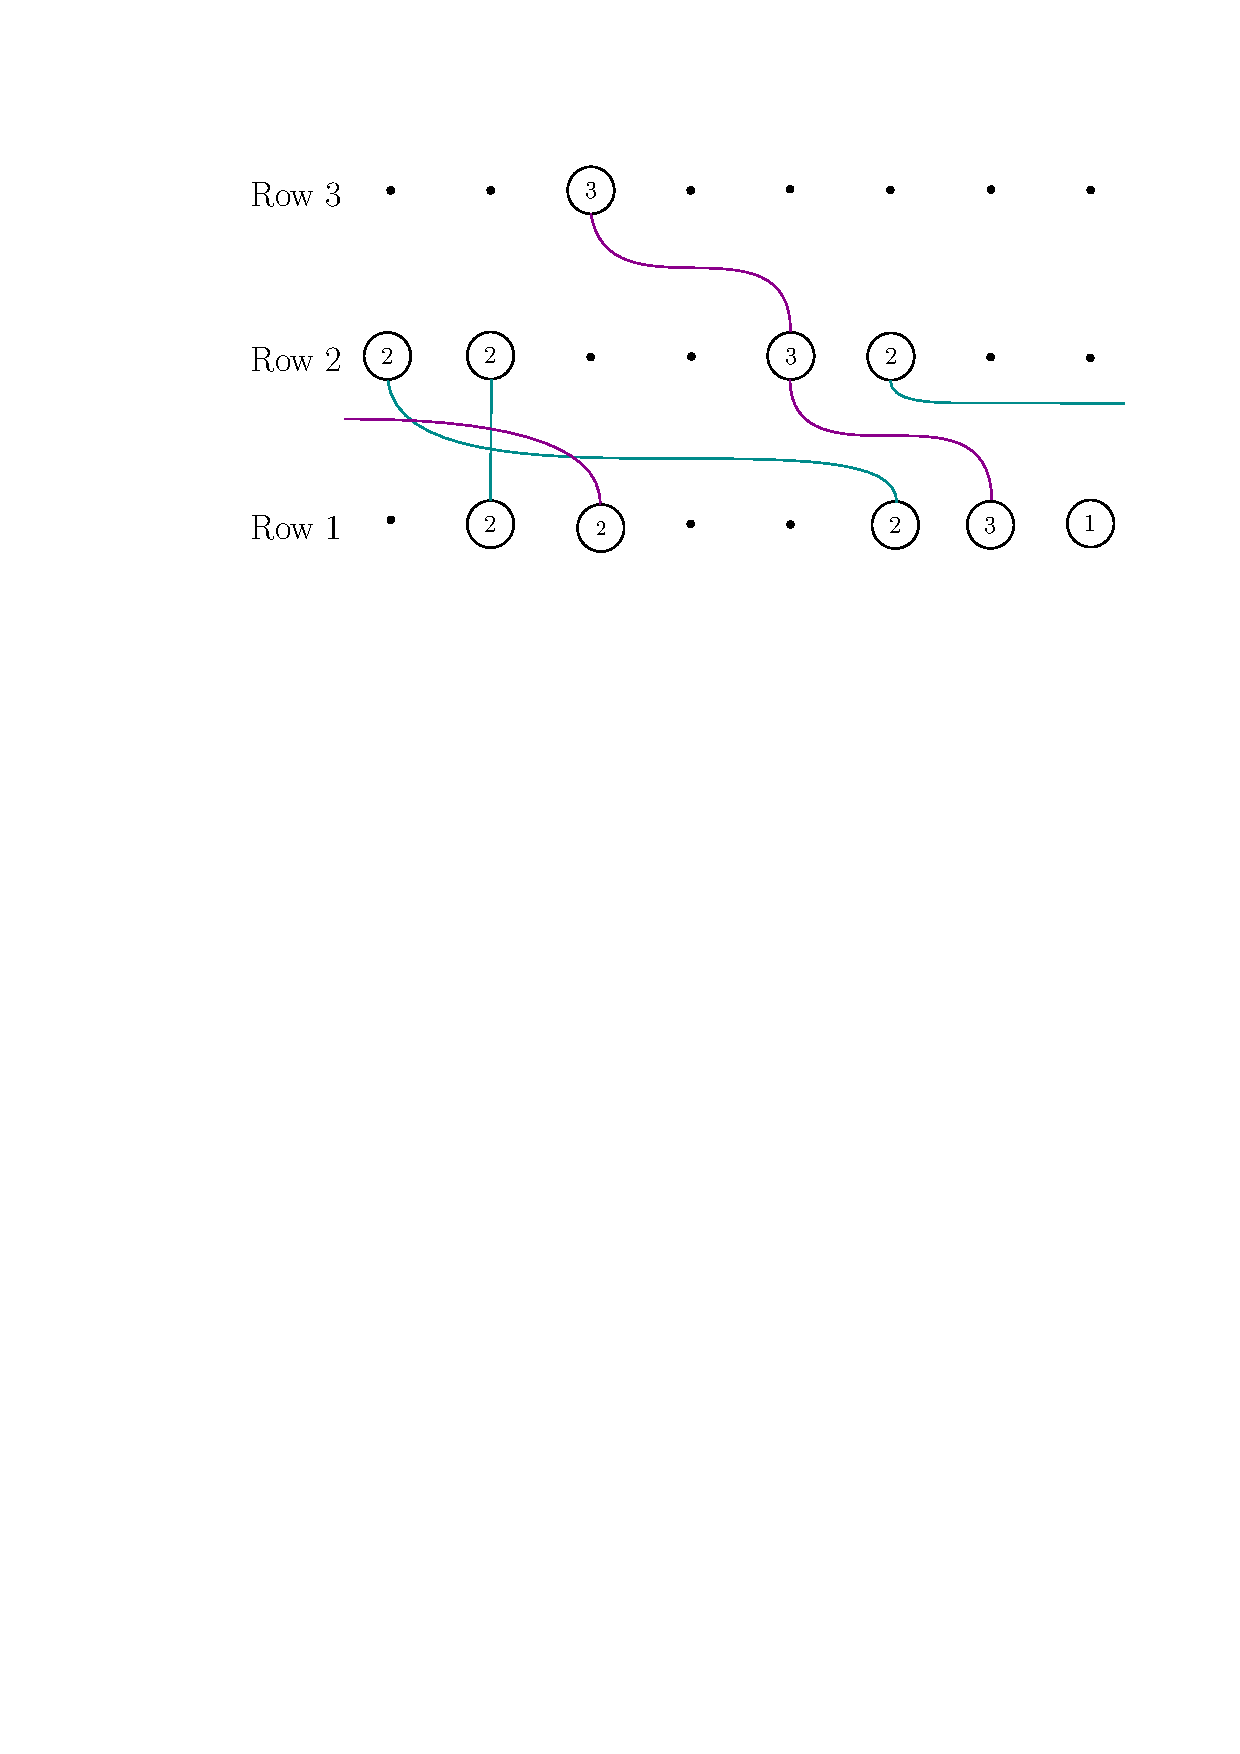
\includegraphics[height=0.19\linewidth,valign=c]{GhostMLQtr2.pdf}$$

\begin{figure}
    \centering
    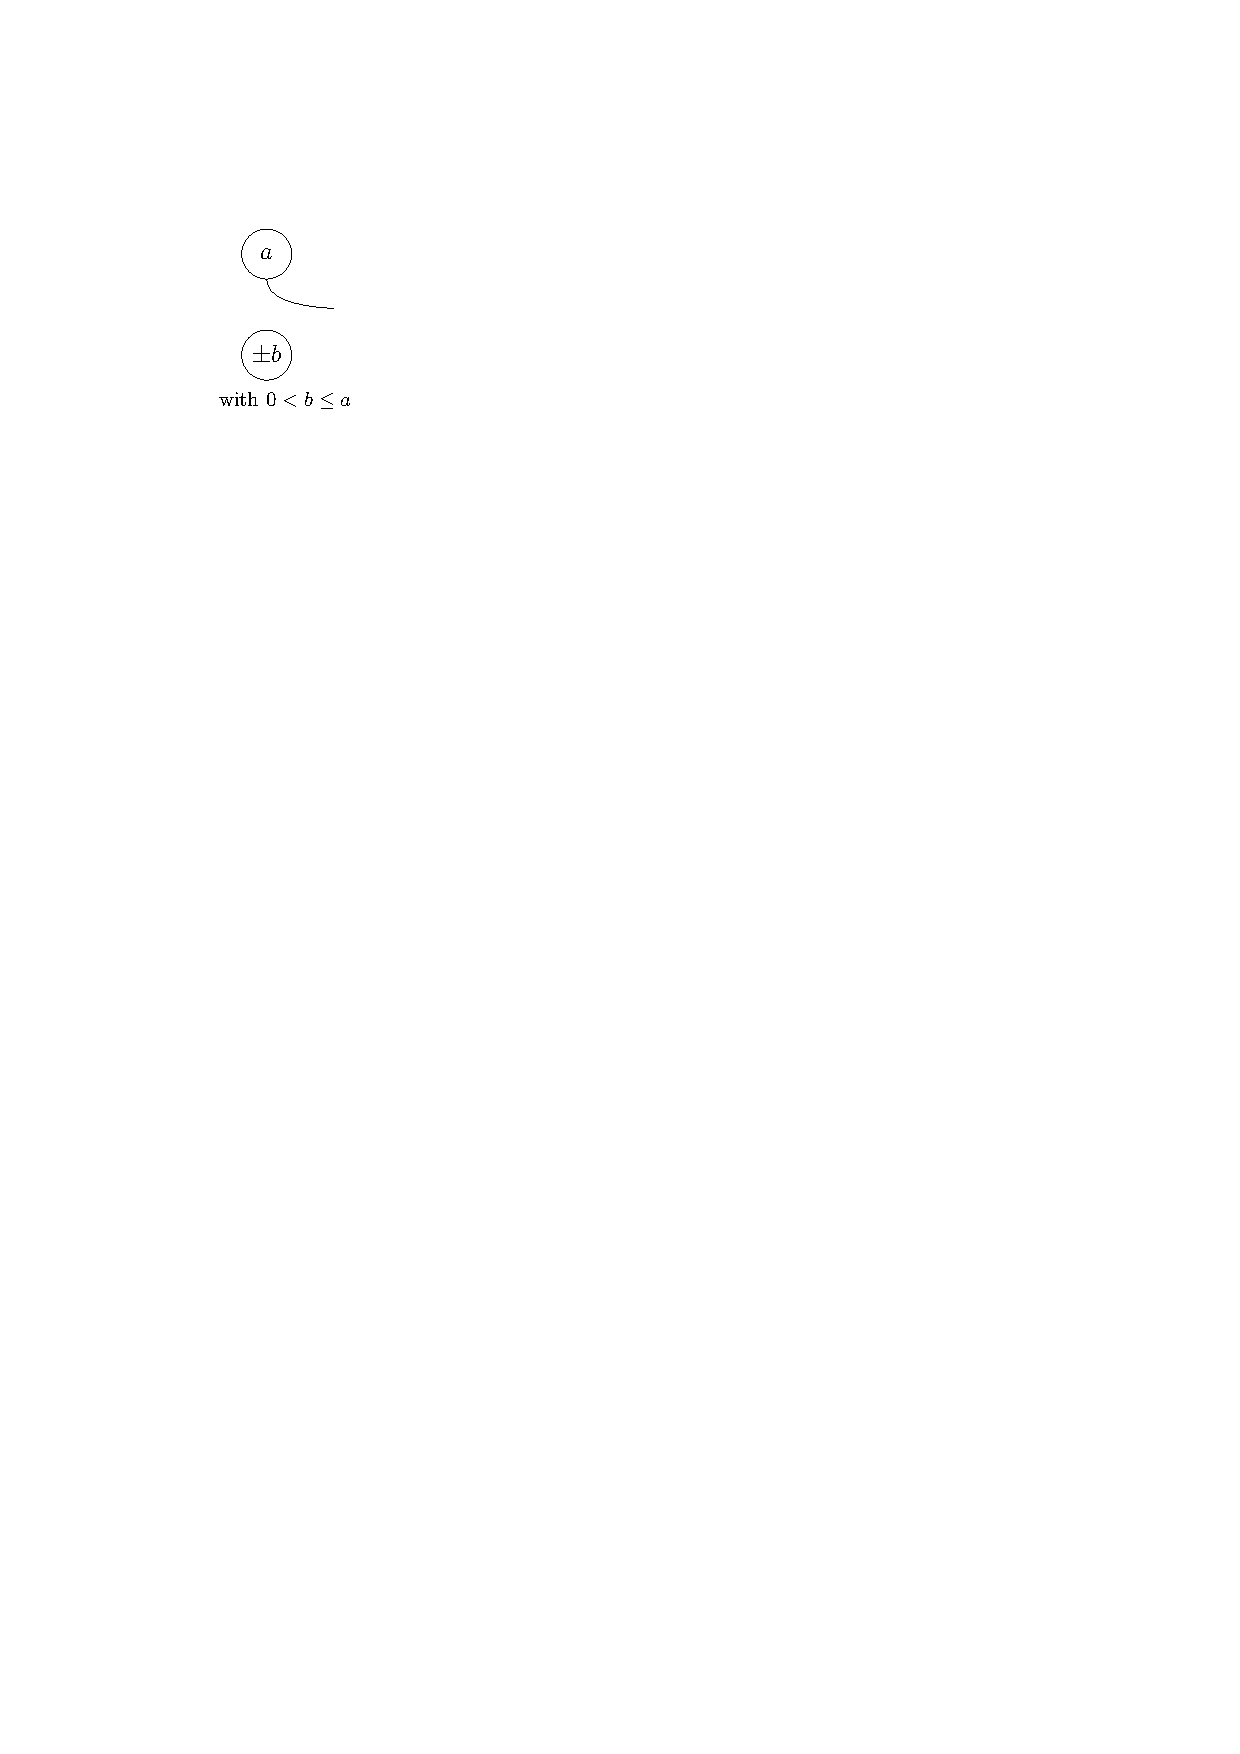
\includegraphics[height=0.14\linewidth]{Forbidden configuration classic.pdf}
    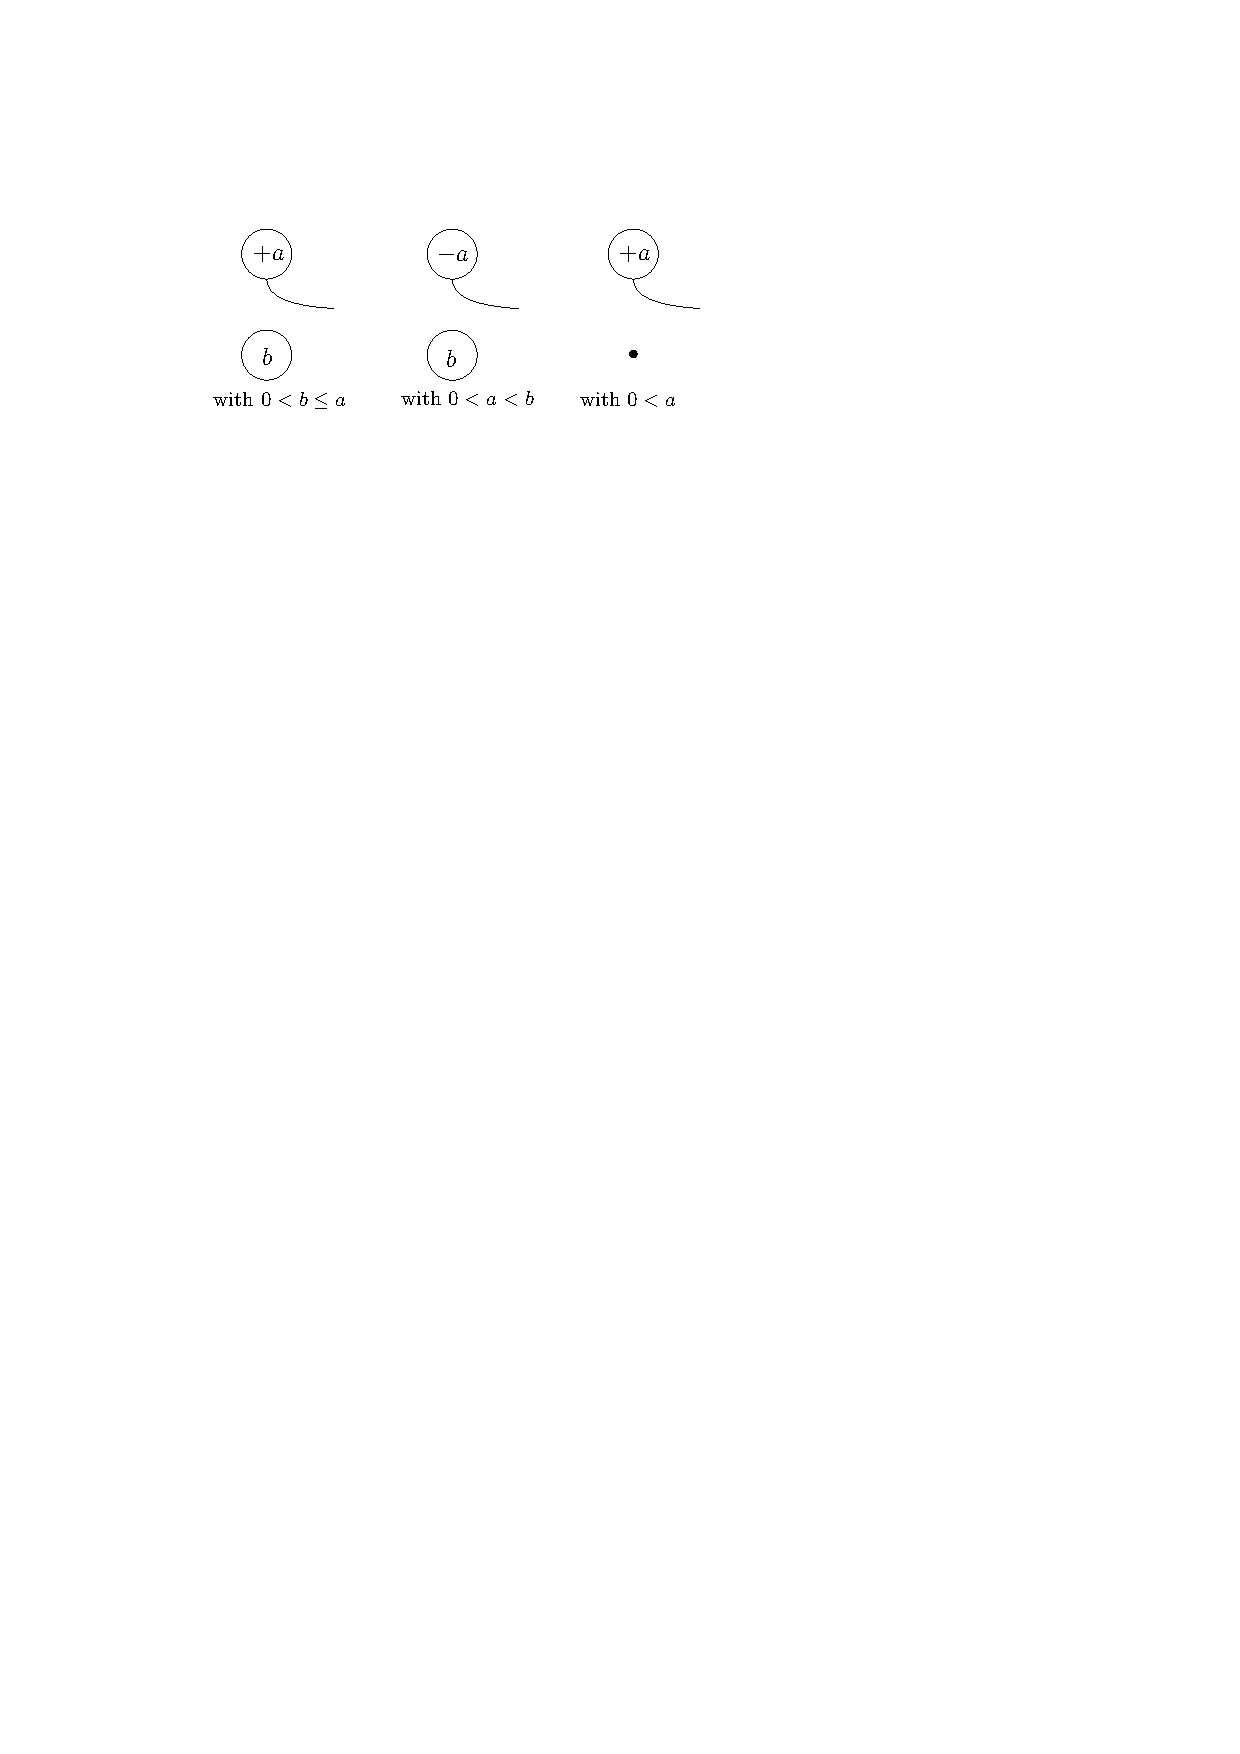
\includegraphics[height=0.14\linewidth]{Forbidden configurations ghost.pdf}
    \caption*{The forbidden configuration for signed multiline queues.}
\end{figure}
\end{frame}

























\begin{frame}{Main result}
    \begin{thm}[BD--Williams]
For any composition $\mu$, we have
$$f^*_\mu(x_1,\dots,x_n;q,t)=\sum_{\substack{\text{signed multiline-queues}\\Q \text{ of type }\mu}}\wt(Q).$$
\vspace{-0.3cm}
As a consequence, for any partition $\lambda$,
$$P^*_\lambda(x_1,\dots,x_n;q,t)=\sum_{\mu\in S_n(\lambda)}\ \sum_{\substack{\text{signed multiline-queues}\\Q \text{ of type }\mu}}\wt(Q).$$
\end{thm}

\pause
The top homogeneous part corresponds to the formula of  Corteel--Mandelshtam--Williams.
\pause 

We also give a tableau formula for $f^*_\mu$ and $P^*_\mu$.
\end{frame}


\begin{frame}{Combinatorial recursion}
\smaller
    \only<1>{$$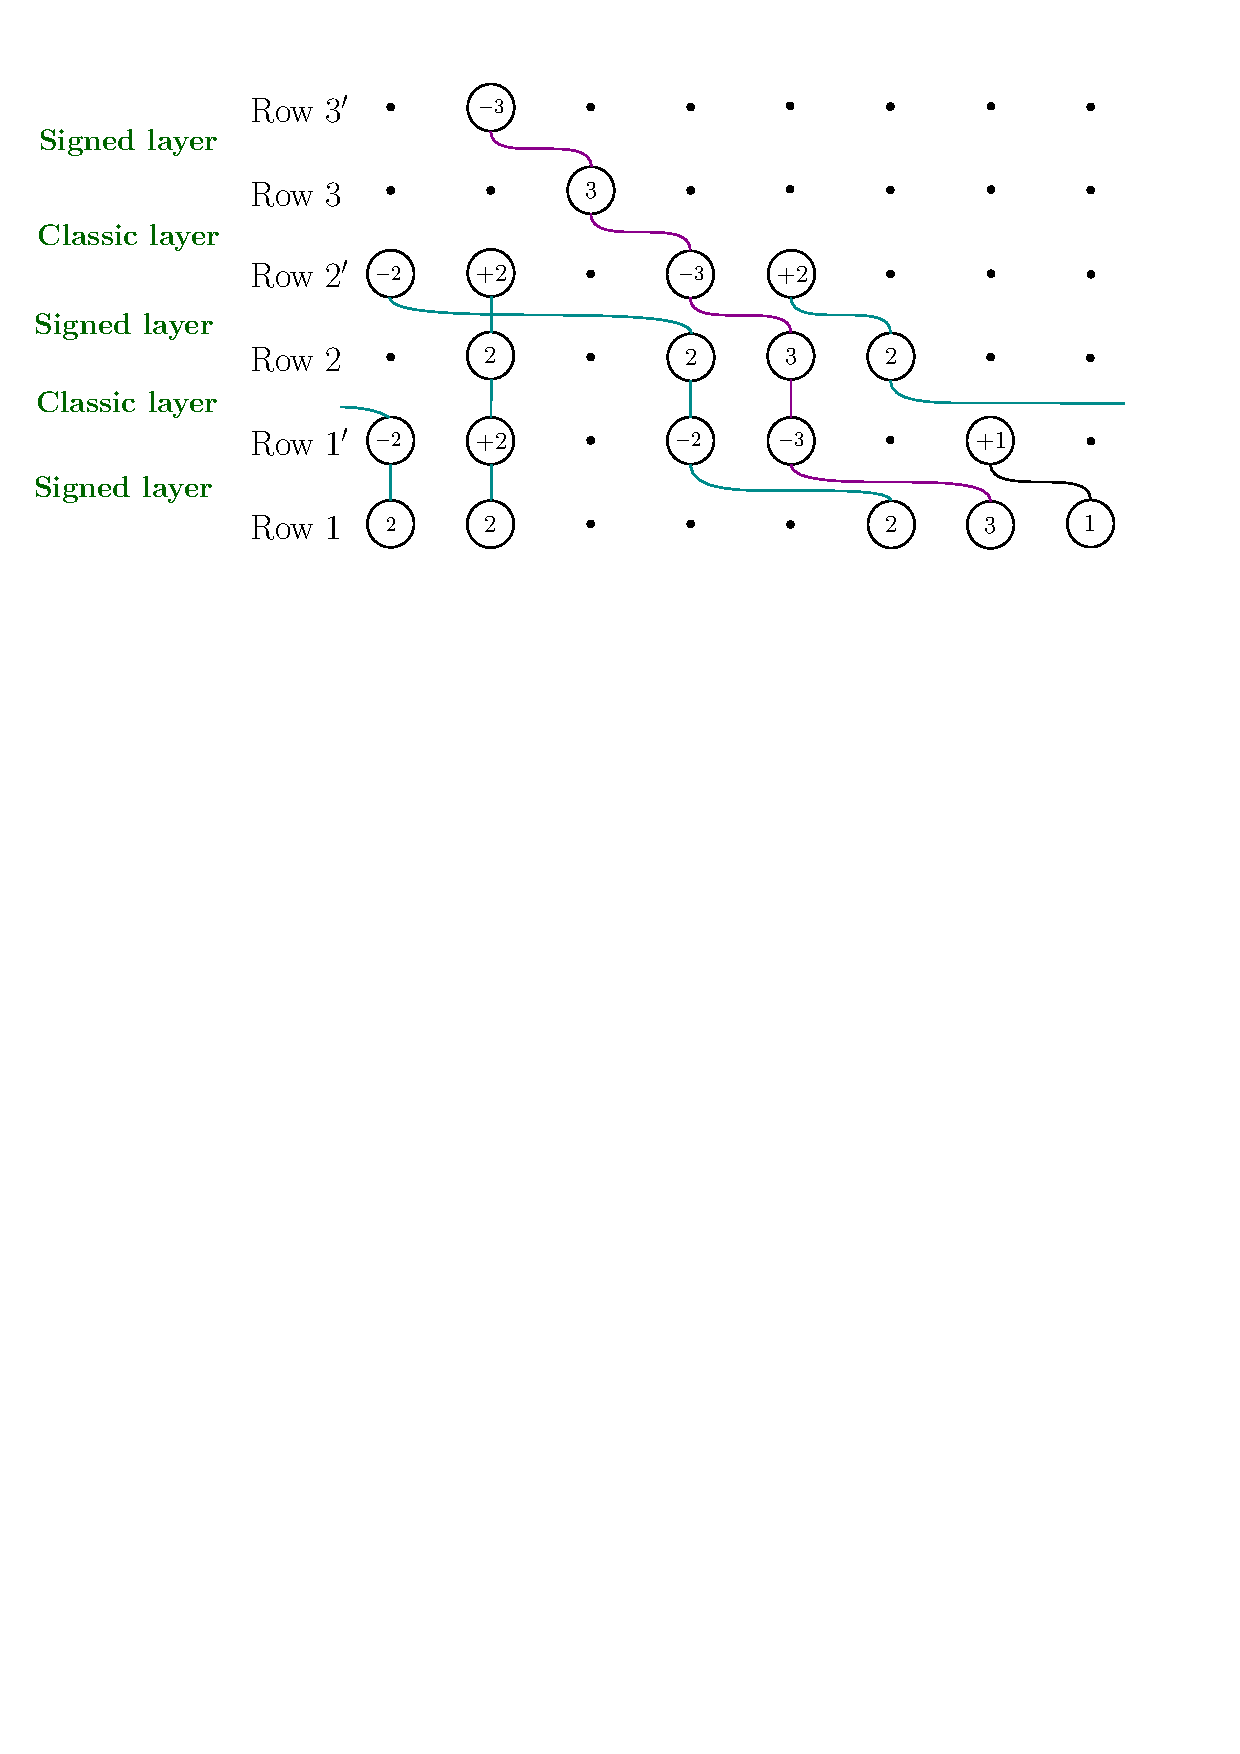
\includegraphics[width=0.45\textwidth,valign=c]{GhostMLQ.pdf}\equiv 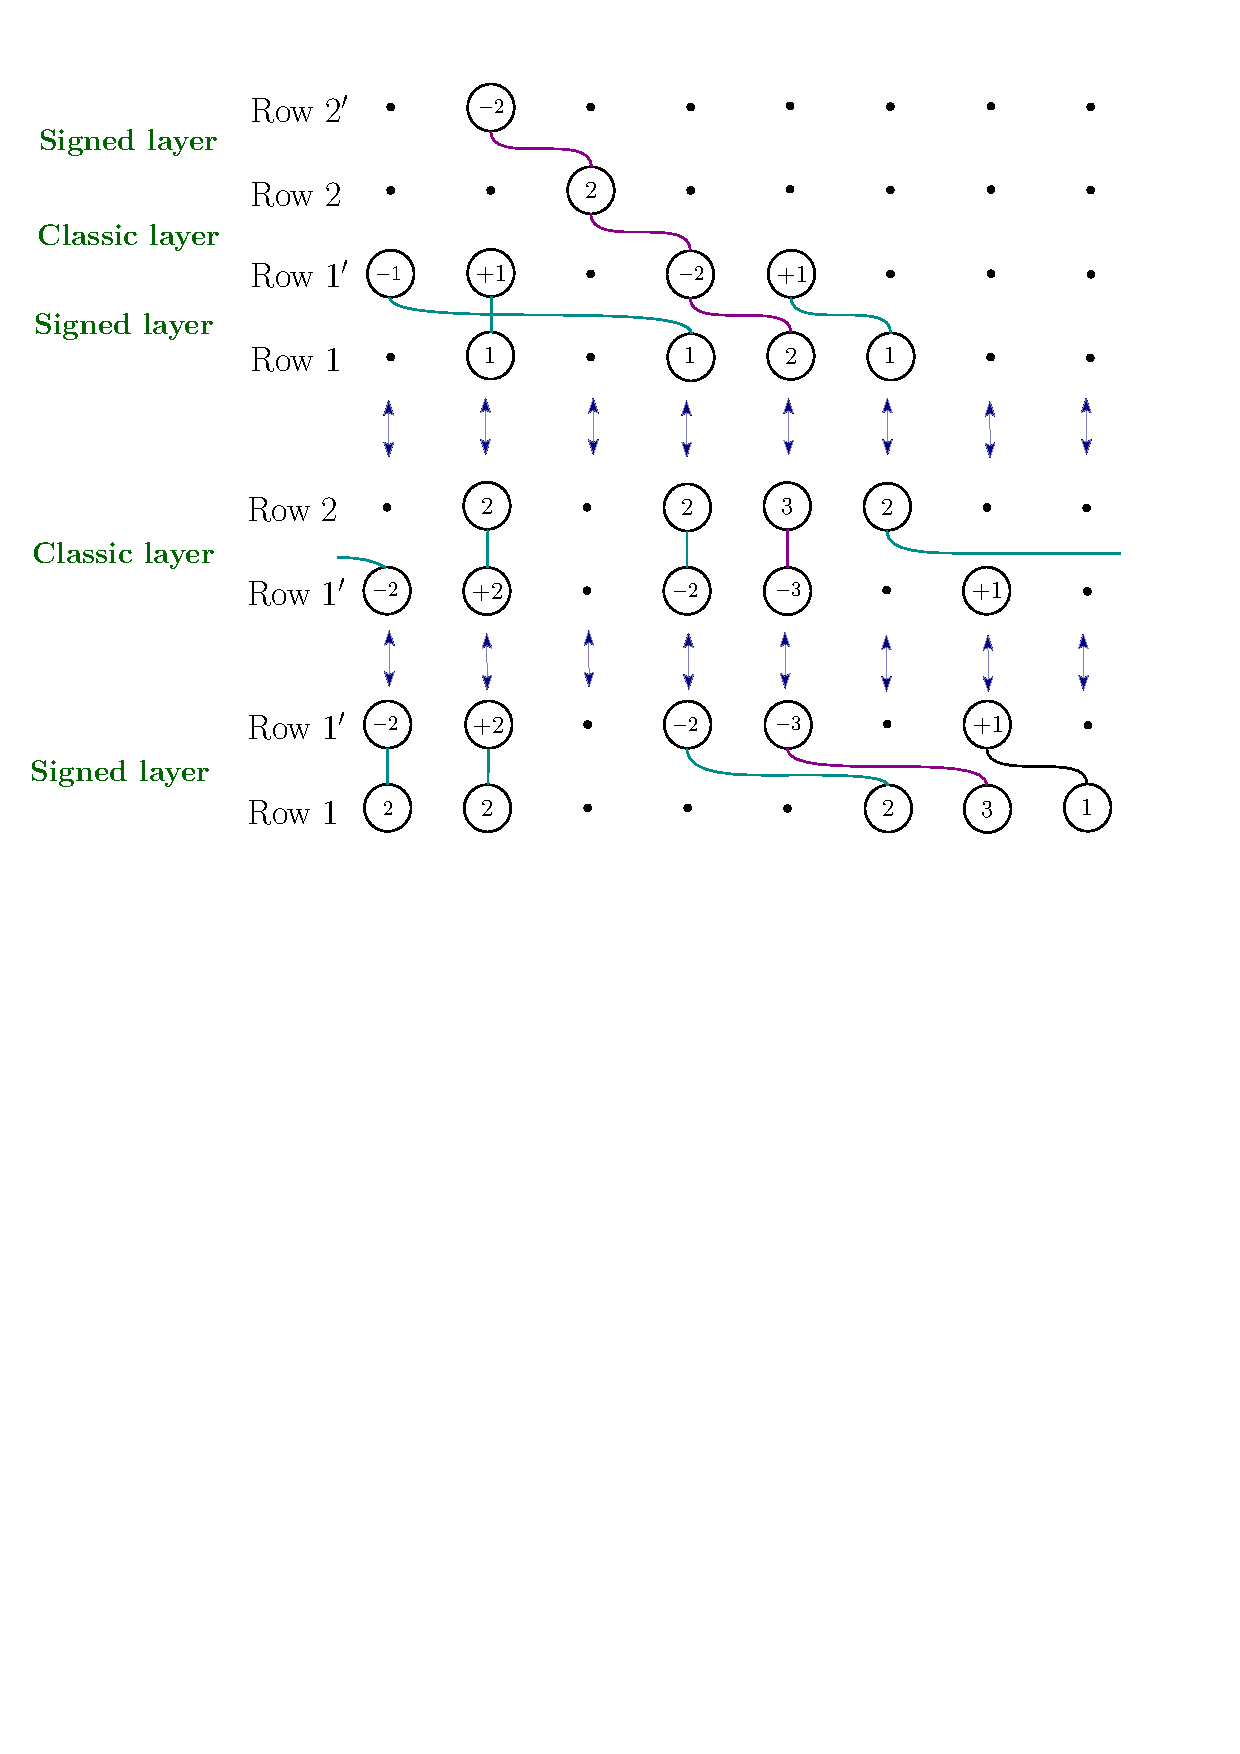
\includegraphics[width=0.45\textwidth,valign=c]{GhostMLQ_decomposed.pdf}.$$}
    \only<2->{$$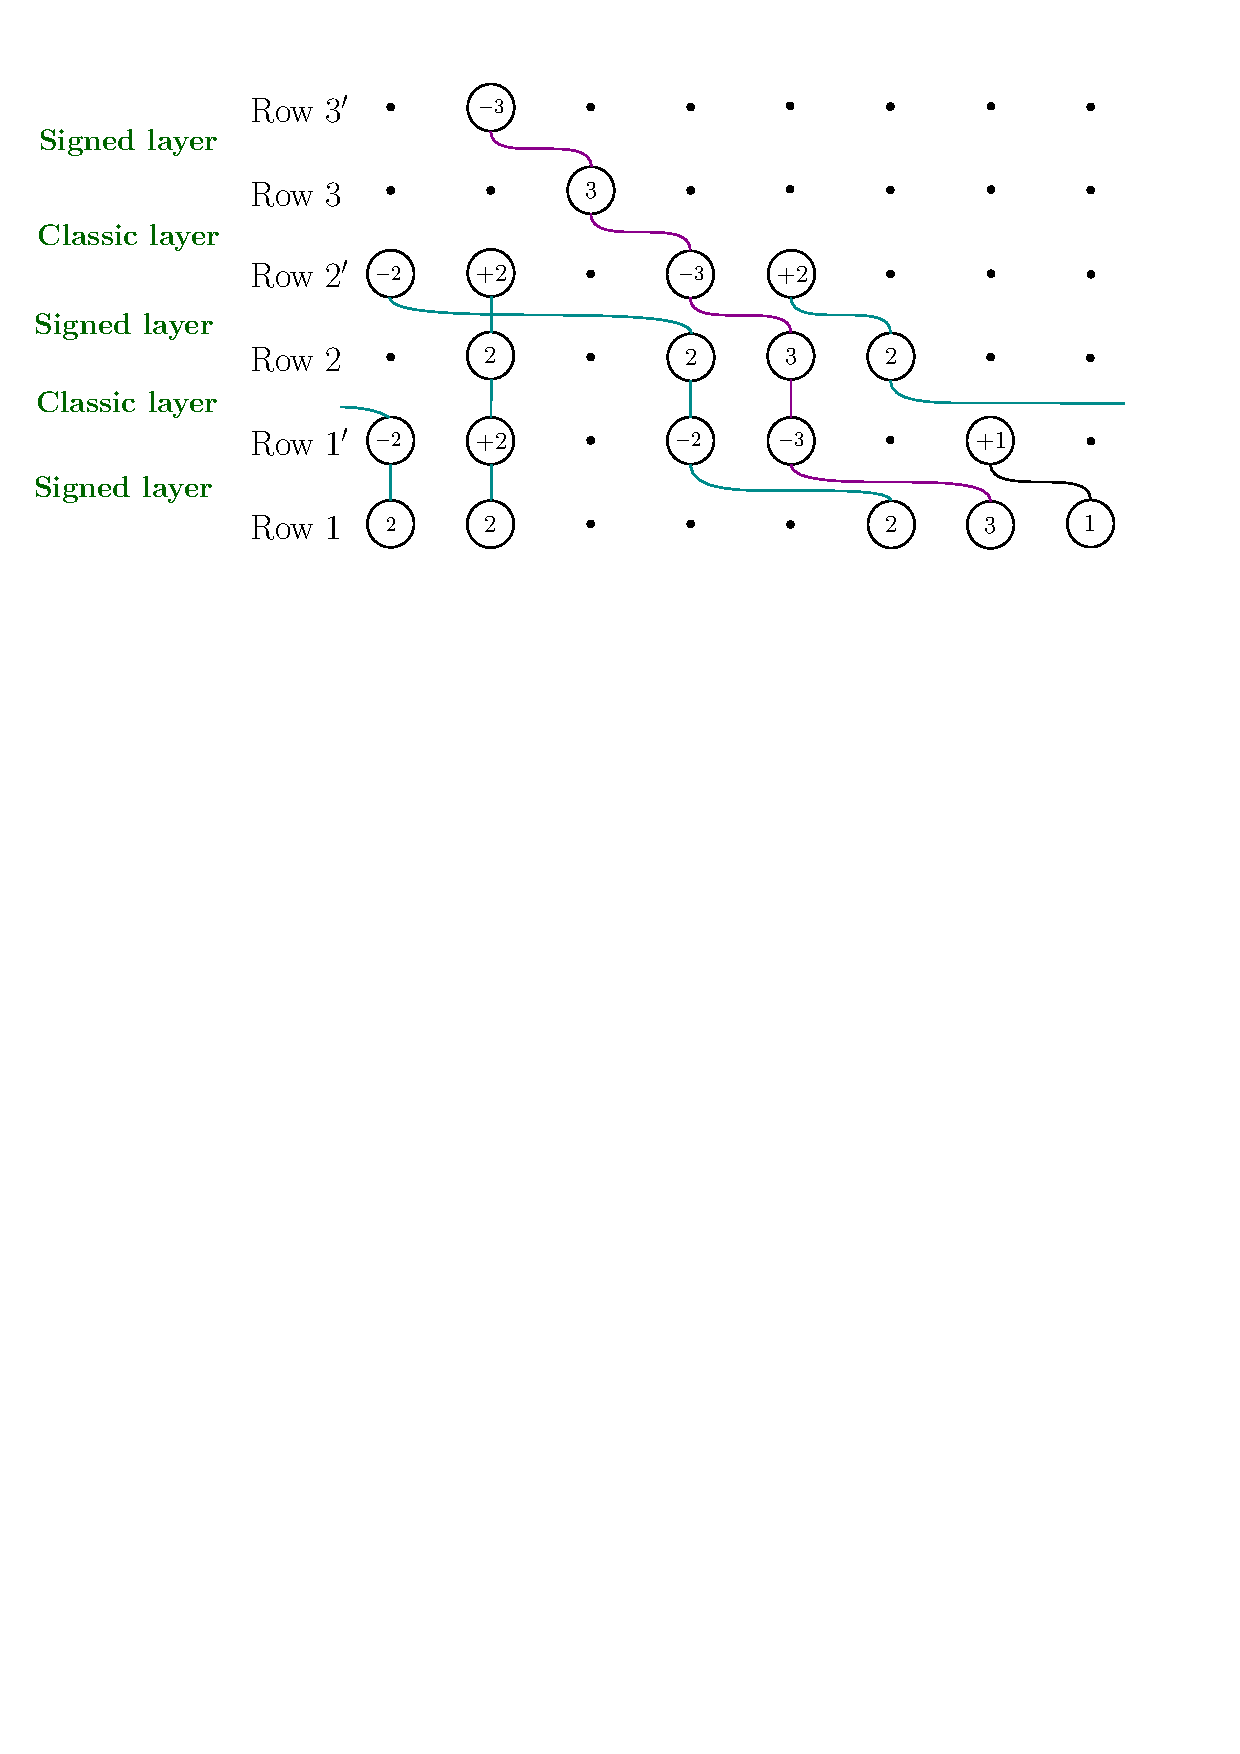
\includegraphics[width=0.45\textwidth,valign=c]{GhostMLQ.pdf}\equiv 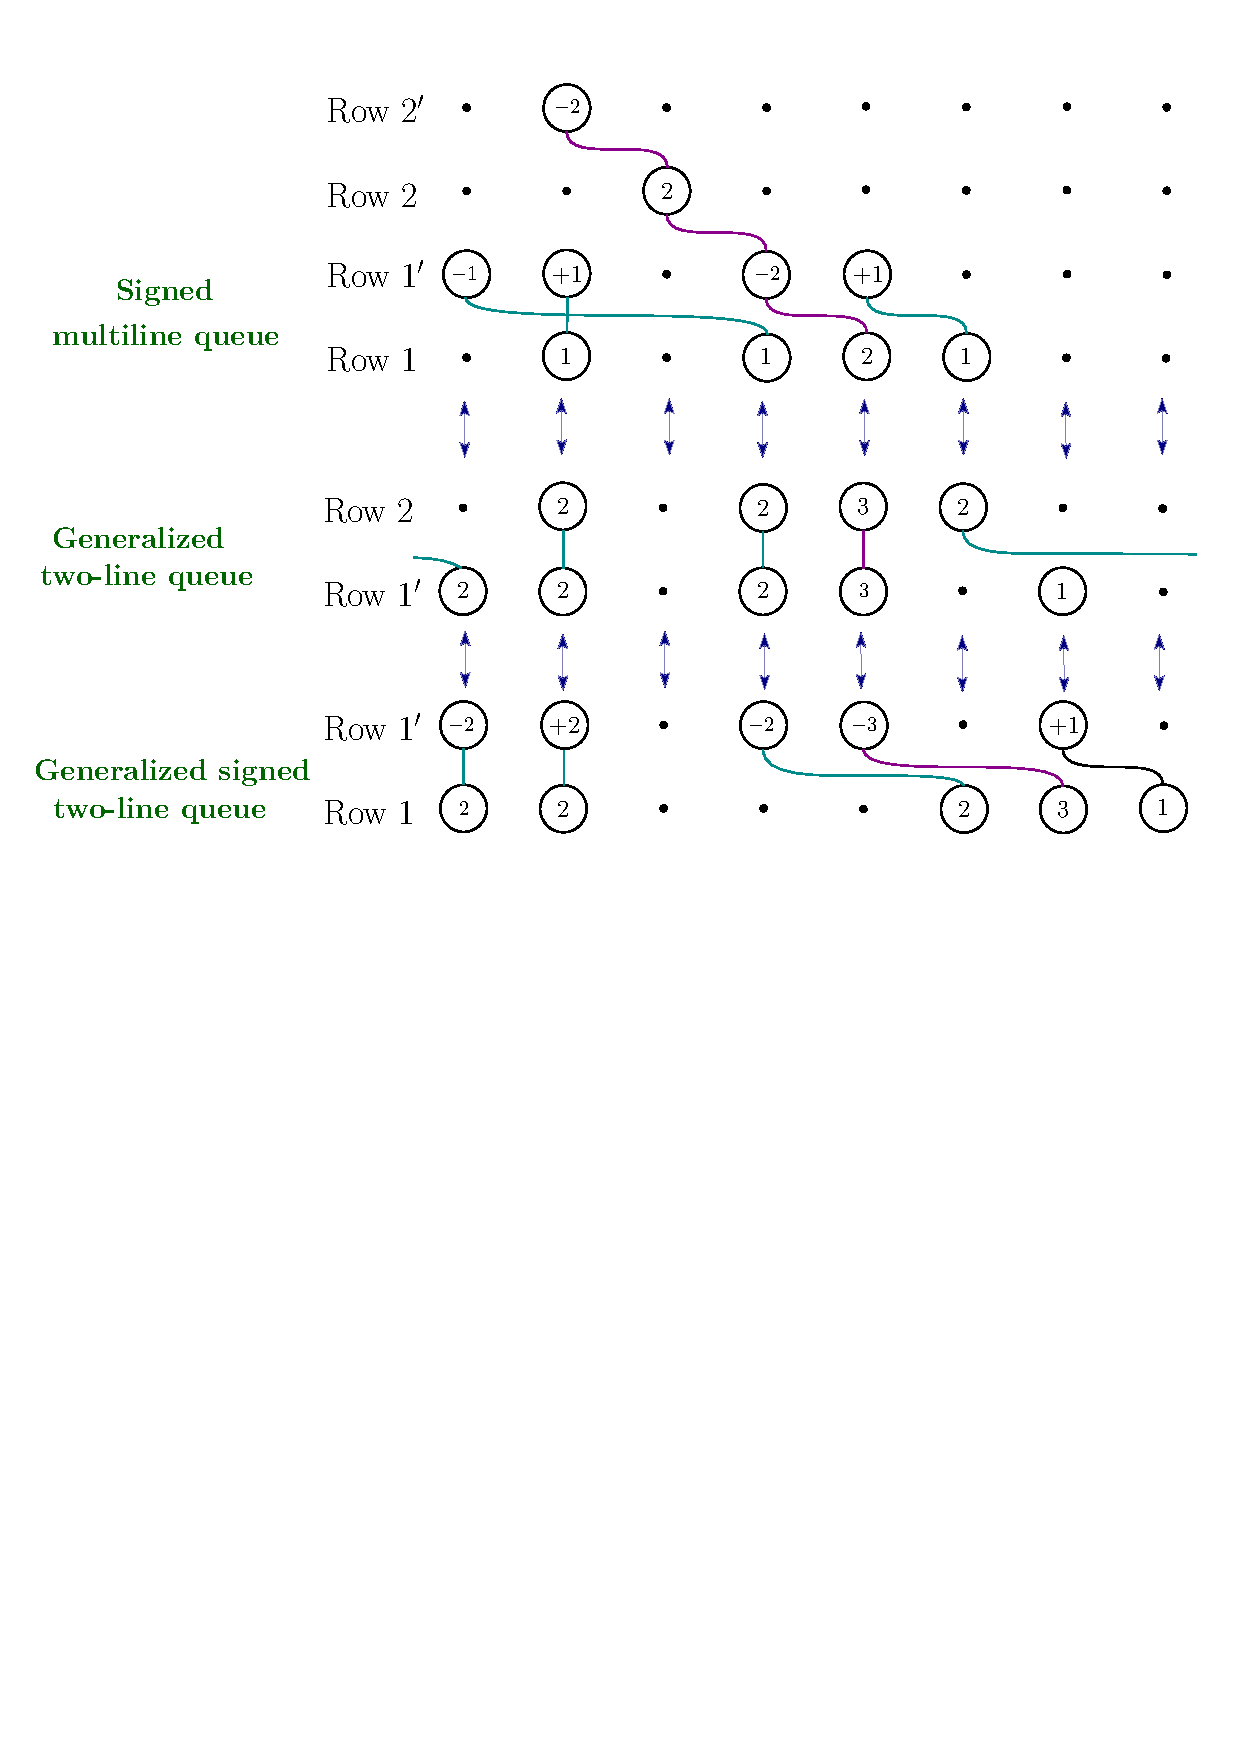
\includegraphics[width=0.45\textwidth,valign=c]{GhostMLQ_decomposed2.pdf}.$$}
\vspace{0.5cm}
\pause 
\pause 
\only<3-4>{
Define the generating function:
$$F^*_\mu(x_1,\dots,x_n;q,t):=\sum_{\substack{\text{signed multiline-queues}\\Q \text{ of type }\mu}}\wt(Q),$$}
\only<3>{
\textbf{Recall:} We want to show that $f^*_\mu=F^*_{\mu}$.}
\pause
\only<4>{
    For  $\lambda,\nu\in \NN^n$, define
    $\GM^\lambda_{\nu}(q,t):=$ the weighted generating functions of generalized two-line queues of bottom row $\nu$, top row $\lambda$,
    
    For  $\mu\in \NN^n$ and $\alpha\in \ZZ^n$, define
    $\GS^\alpha_{\mu}(t):=$ the weighted generating functions of generalized signed two-line queues of bottom row $\mu$, top row $\alpha$,}
\pause
    We have 
    $$F^*_\mu(x_1,\dots,x_n)=\sum_{\alpha\in \ZZ^n}\sum_{\lambda\in \NN^n} \GS_\mu^\alpha \wt_{\alpha} \GM_{|\alpha|}^\lambda  q^{|\lambda^-|}F^*_{\lambda-}\left(\frac{x_1}{q},\dots,\frac{x_n}{q}\right)$$
    where $\lambda^-$ is the composition obtained from $\lambda$ by substracting 1 from each non zero entry,\\
    and $\wt_{\alpha}=\prod_{i: \alpha_i>0}x_i\prod_{i:\alpha_i<0}\frac{-1}{t^{n-1}}$: ball weight in row $1'$.
\end{frame}


\begin{frame}{Algebraic recursion}

    We want to prove that the polynomials $f^*_\mu$ satisfy the same recursion.
    \pause
    
    We start by the \textbf{packed case}. Define $\Pack(k,n)$ as the set of compositions $\mu\in\NN^n$ such that $\mu_i\neq 0$ if and only if $1\leq i\leq k$.

    
    \textcolor{uibred}{\textbf{Example:}} $(2,3,1,0,0)\in \Pack(3,5)$.
    
    \only<3>{
    \begin{thm}
        If $\mu\in \Pack(k,n)$, then the polynomial $f^*_\mu$ is divisible by $\prod_{1\leq i\leq k}\left(x_i-\frac{1}{t^{n-1}}\right)$. Moreover,
        $$f^*_\mu=\prod_{1\leq i\leq k}\left(x_i-\frac{1}{t^{n-1}}\right)\sum_{\substack{\nu\in \NN^n\\|\nu|\leq |\mu|-k
        }}a^\nu_{\mu}(q,t)f^*_\nu,$$
    \end{thm}}
    \only<3>{
    \textbf{Hint:} A polynomial $R(x_1,\dots,x_n)$ is identically 0 if and only if $R(\widetilde \nu)=0$ for any $\nu\in \NN^n$.}
    
\pause \pause 
    \begin{thm}
        If $\mu\in \Pack(k,n)$, then the polynomial $f^*_\mu$ is divisible by $\prod_{1\leq i\leq k}\left(x_i-\frac{1}{t^{n-1}}\right)$. Moreover,
        $$f^*_\mu(x_1,\dots,x_n)=\prod_{1\leq i\leq k}\left(x_i-\frac{1}{t^{n-1}}\right)\sum_{\substack{\nu\in \NN^n\\|\nu|\color{uibred}=\color{black} |\mu|-k}
        } a^\nu_{\mu}(q,t)q^{|\nu|}f^*_\nu\left(\frac{x_1}{q},\dots,\frac{x_n}{q}\right).$$
        \pause
        We also have $a_\mu^{\nu-}=\GM_\mu^{\nu}.$
    \end{thm}
    \only<5>{
    \textbf{Hint:} Extract the top homogeneous coefficient and use the formula of Corteel--Mandelshtam--Williams.}
    \pause
    We check that this recursion agrees with the combinatorial recursion.
\end{frame}



\begin{frame}{Hecke operators}
    For $1\leq i\leq n-1$, define the operator 
\begin{equation*}
T_i:=t-\frac{tx_i-x_{i+1}}{x_i-x_{i+1}}(1-s_i).
\end{equation*}
\pause
These operators satisfy the relations of the Hecke algebra of type $A_{n-1}$
\begin{equation*}
\begin{array}{ll}
(T_i-t)(T_i+1)=0 & \text{for $1\leq i \leq n-1$}\\
 T_iT_{i+1}T_i=T_{i+1}T_iT_{i+1}    & \text{for $1\leq i \leq n-2$}\\
 T_iT_j=T_jT_i    & \text{for $ |i-j| > 1$}.\\
\end{array}
\end{equation*}

\begin{prop}
        For any composition $\mu$, we have
    \begin{equation*}
                T_i f^*_{\mu}=\begin{cases}
                    f^*_{s_i\mu} &\text{if $\mu_i>\mu_{i+1}$},\\
                    tf^*_{\mu} & \text{if $\mu_i=\mu_{i+1}$},\\
                    tf^*_{s_i\mu}-(1-t)f^*_{\mu}&\text{ if $\mu_i<\mu_{i+1}$}
                \end{cases}.
    \end{equation*}
\end{prop}
\vspace{-0.2cm}
Any $f^*_\mu$ can be obtained from the packed case using Hecke operators.
\end{frame}

\begin{frame}{Unpacking procedure}
\only<-1>{
    \textbf{Recall:} We want to prove that 
        $$f^*_\mu(x_1,\dots,x_n)=\sum_{\alpha\in \ZZ^n}\sum_{\lambda\in \NN^n} \GM_\mu^\alpha \wt_{\alpha}\GS_{|\alpha|}^\lambda q^{|\lambda^-|}f^*_{\lambda-}\left(\frac{x_1}{q},\dots,\frac{x_n}{q}\right),$$
        checked for packed $\mu$.
        }
        
        \pause 
        \vspace{0.2cm}
        \begin{prop}
        \smaller
        Fix $\mu$, such that $\mu_i>0$ and $\mu_{i+1}=0$.
            Assume that $$f^*_\mu(x_1,\dots,x_n)=\sum_{\alpha\in \ZZ^n}\sum_{\lambda\in \NN^n} b_\mu^\alpha \wt_{\alpha} \GM_{|\alpha|}^\lambda q^{|\lambda^-|}f^*_{\lambda-}\left(\frac{x_1}{q},\dots,\frac{x_n}{q}\right),$$
            for some coefficients $(b_\mu^\alpha)_{\alpha\in \ZZ^n}.$
        We then apply $T_i$ to obtain an equation for $f^*_{\text{\textcolor{uibred}{$s_i \mu$}}}$:
        $$f^*_{\text{\textcolor{uibred}{$s_i \mu$}}}(x_1,\dots,x_n)=\sum_{\alpha\in \ZZ^n}\sum_{\lambda\in \NN^n} b_{\text{\textcolor{uibred}{$s_i \mu$}} }^\alpha \wt_{\alpha}\GM_{|\alpha|}^\lambda q^{|\lambda^-|}f^*_{\lambda-}\left(\frac{x_1}{q},\dots,\frac{x_n}{q}\right),$$
        \vspace{-0.4cm}
        
        where $b^\alpha_{s_i \mu}=$
            \pause

        \vspace{-0.4cm}
        \begin{align*}
    &t b^\alpha_\mu 
    &&\text{if $\alpha_i=\alpha_{i+1}$},\\
    &       t b_\mu^{s_i\alpha}
    &&\text{if $\alpha_i>\alpha_{i+1}\geq 0$, $-\alpha_i>-\alpha_{i+1}>0$,  $\alpha_i>-\alpha_{i+1}> 0$}\\
    &&&\text{$-\alpha_{i+1}>\alpha_{i}=0$ or $\alpha_i=-\alpha_{i+1}>0$}\\
    &        b_\mu^{s_i\alpha}-(1-t)b^\alpha_{\mu}
    &&\text{if $\alpha_{i+1}>\alpha_{i}\geq 0$, 
            $-\alpha_{i+1}>-\alpha_{i}> 0$},\\
           & &&\text{$-\alpha_i=\alpha_{i+1}>0$ or $\alpha_{i+1}>-\alpha_{i}> 0$,}\\
    &         tb_\mu^{s_i\alpha}-(1-t)b_\mu^{\alpha}
             &&\text{if $-\alpha_i>\alpha_{i+1}=0$,}\\
    &         tb_\mu^{s_i\alpha}-(1-t)\left(b_\mu^{\alpha}-b^{\dots,-\alpha_i,-\alpha_{i+1},\dots}_\mu\right)\hspace{-0.3cm}
             &&\text{if $-\alpha_i>\alpha_{i+1}> 0$},\\
    &         b_\mu^{s_i\alpha}-(1-t)G^{\dots,-\alpha_i,-\alpha_{i+1},\dots}_\mu
             &&\text{if $-\alpha_{i+1}>\alpha_{i}>0$.}\\
\end{align*}
\vspace{-0.9cm}
        \end{prop}
\end{frame}


\begin{frame}{Unpacking procedure}
    We check that the combinatorial coefficients $\GS_\mu^\alpha$ satisfy the recursion obtained from the Hecke algebra.

    \textbf{Example:} Let's check that if $\alpha_i=\alpha_{i+1}=0$, we have
    $\GS_{s_i \mu}^\alpha=t\GS_{\mu}^\alpha$.

    
    \begin{columns}
\column{0.45\textwidth}\smaller
\begin{figure}
    \centering
    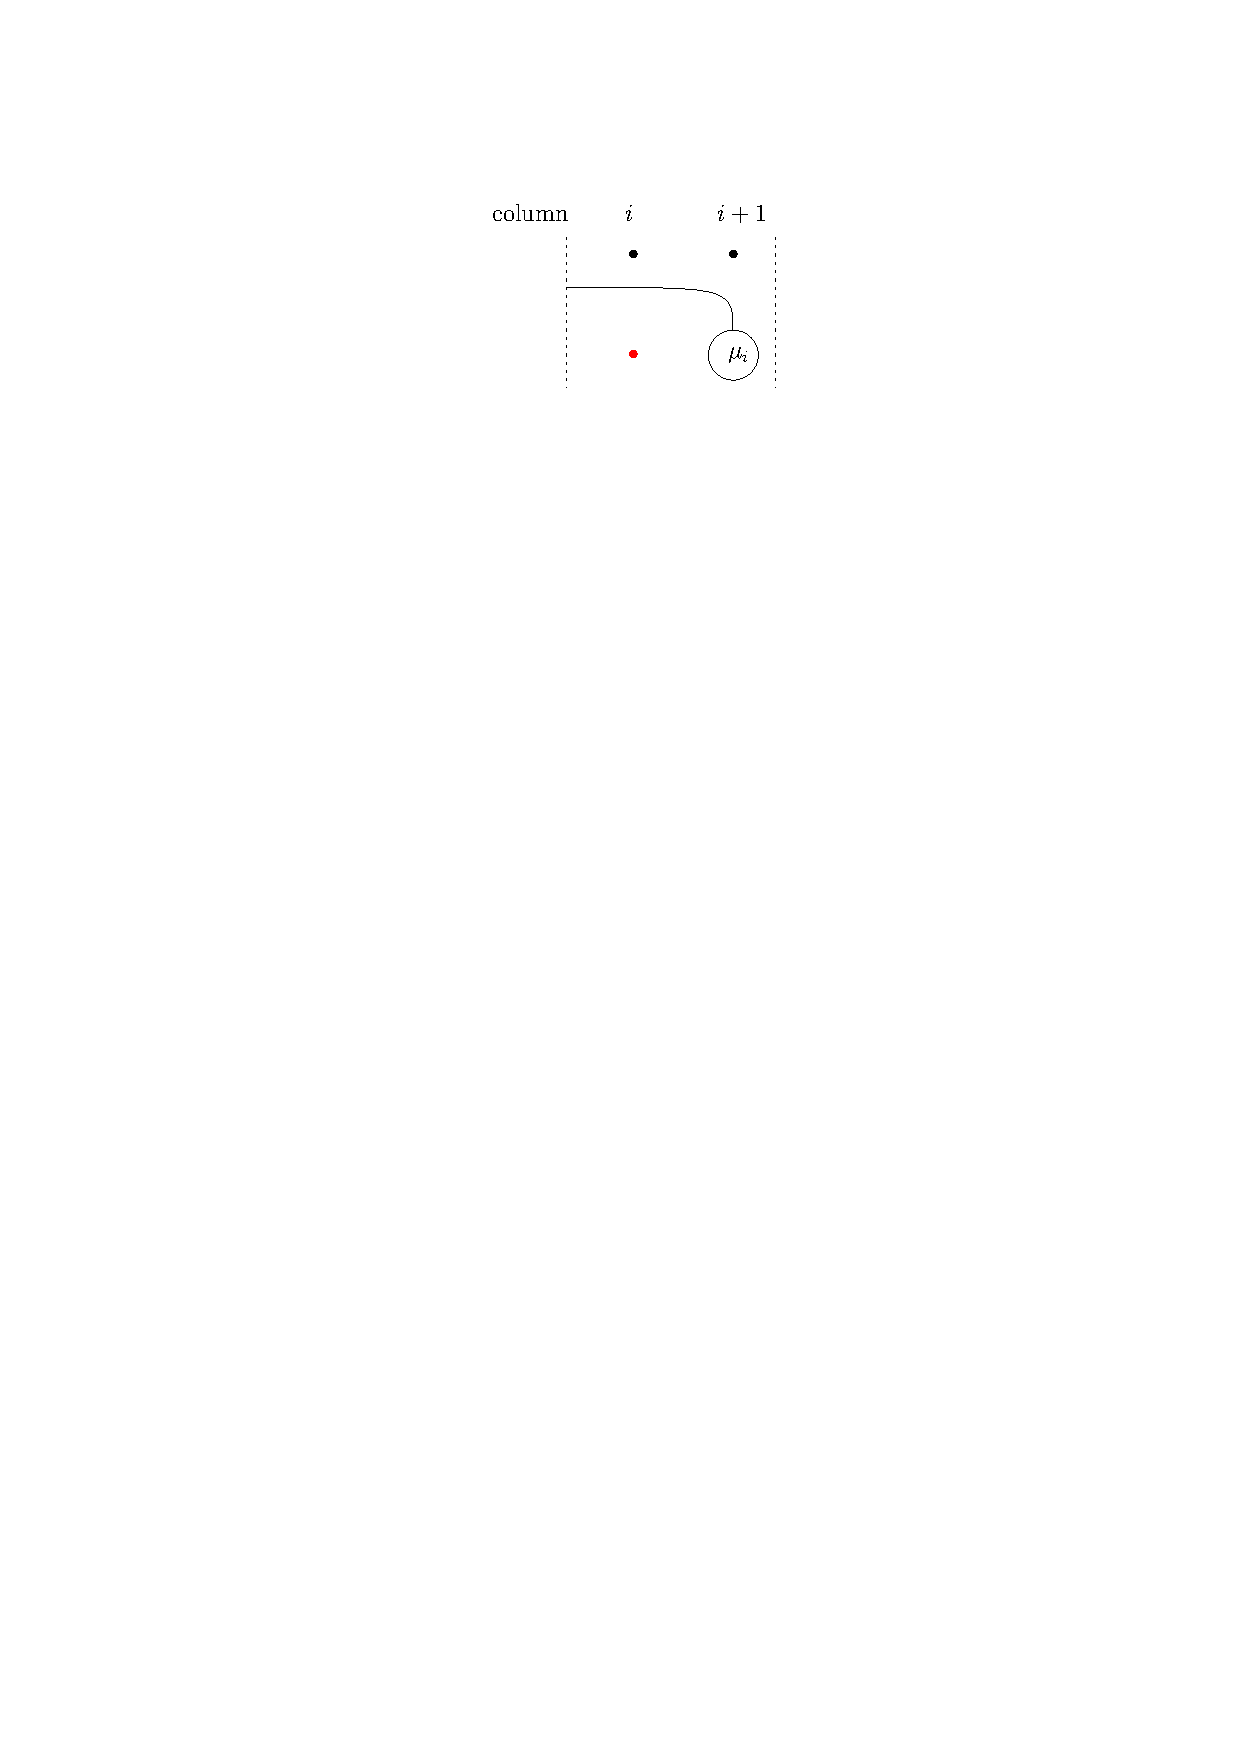
\includegraphics[width=0.6\linewidth]{GTLQ2.pdf}
    \caption*{A generalized signed two-line queue with bottom row $s_i\mu$ and top row $\alpha$:
}
\end{figure}
\column{0.45\textwidth}
\begin{figure}
    \centering
    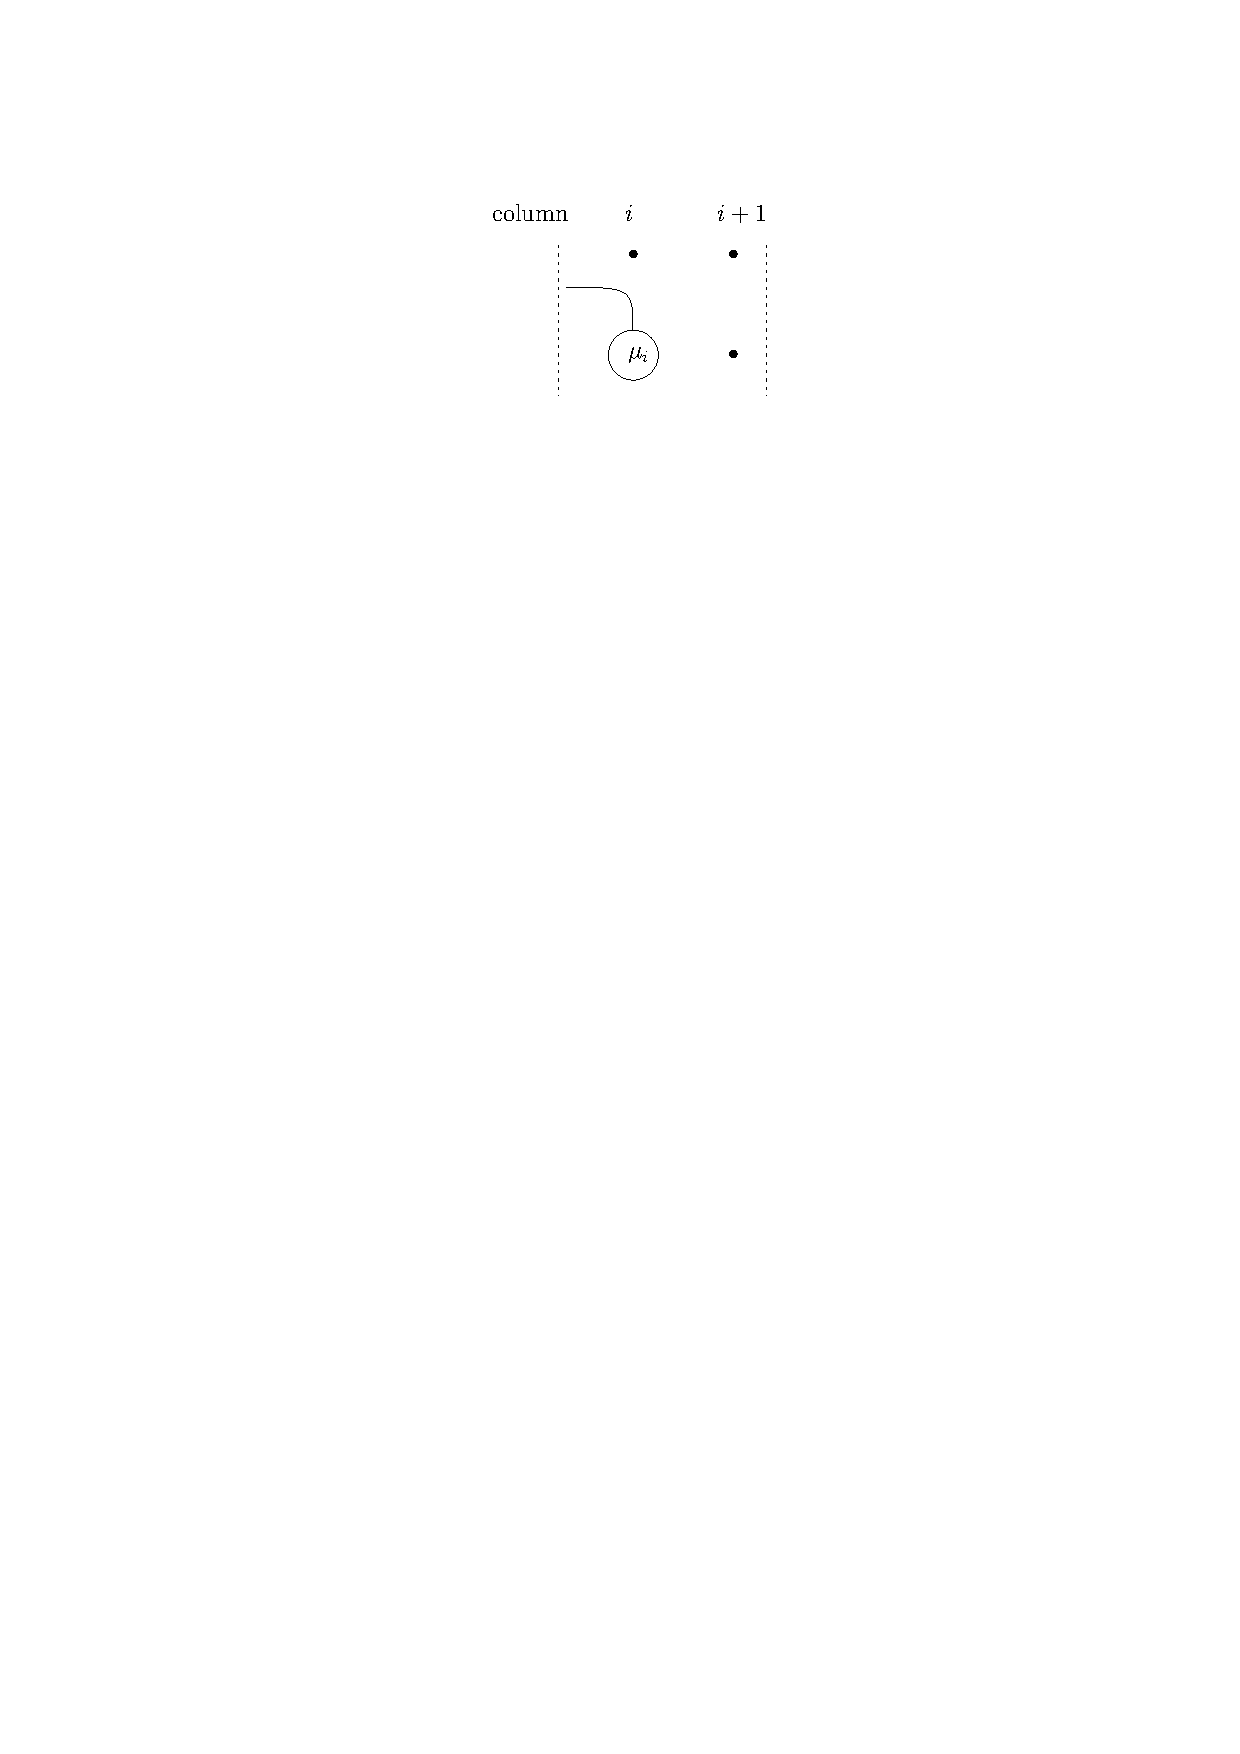
\includegraphics[width=0.6\linewidth]{GTLQ.pdf}
    \caption*{A generalized signed two-line queue of bottom row $\mu$ and top row $\alpha$:}
\end{figure}
\end{columns}
The \textcolor{uibred}{empty} statistic of the pairing in the diagram increases by 1 when we go from the right figure to the left one.

\end{frame}

\begin{frame}{Application: Factorization property}
\textbf{Fact:} $$P_{1^k}(x_1,\dots,x_n;q,t)=e_k(x_1,\dots,x_n):=\sum_{ S\in {\llbracket n \rrbracket \choose k}}
\prod_{i\in S}x_i,$$
\textbf{\textcolor{uibred}{Example:}} For $n=3$ and $k=2$,
$$e_2(x_1,x_2,x_3)=x_1x_2+x_1x_3+x_2x_3.$$
\pause 
\vspace{-0.2cm}
\begin{thm}[Macdonald]
Fix a partition $\lambda$ with $\lambda_1=m$. Then
$$P_\lambda(x_1,\dots,x_n;q=1,t)=e_{\lambda'_1}\dots e_{\lambda'_{m}}.$$
\end{thm}
\vspace{-0.2cm}
\only<2>{
\begin{figure}
    \centering
    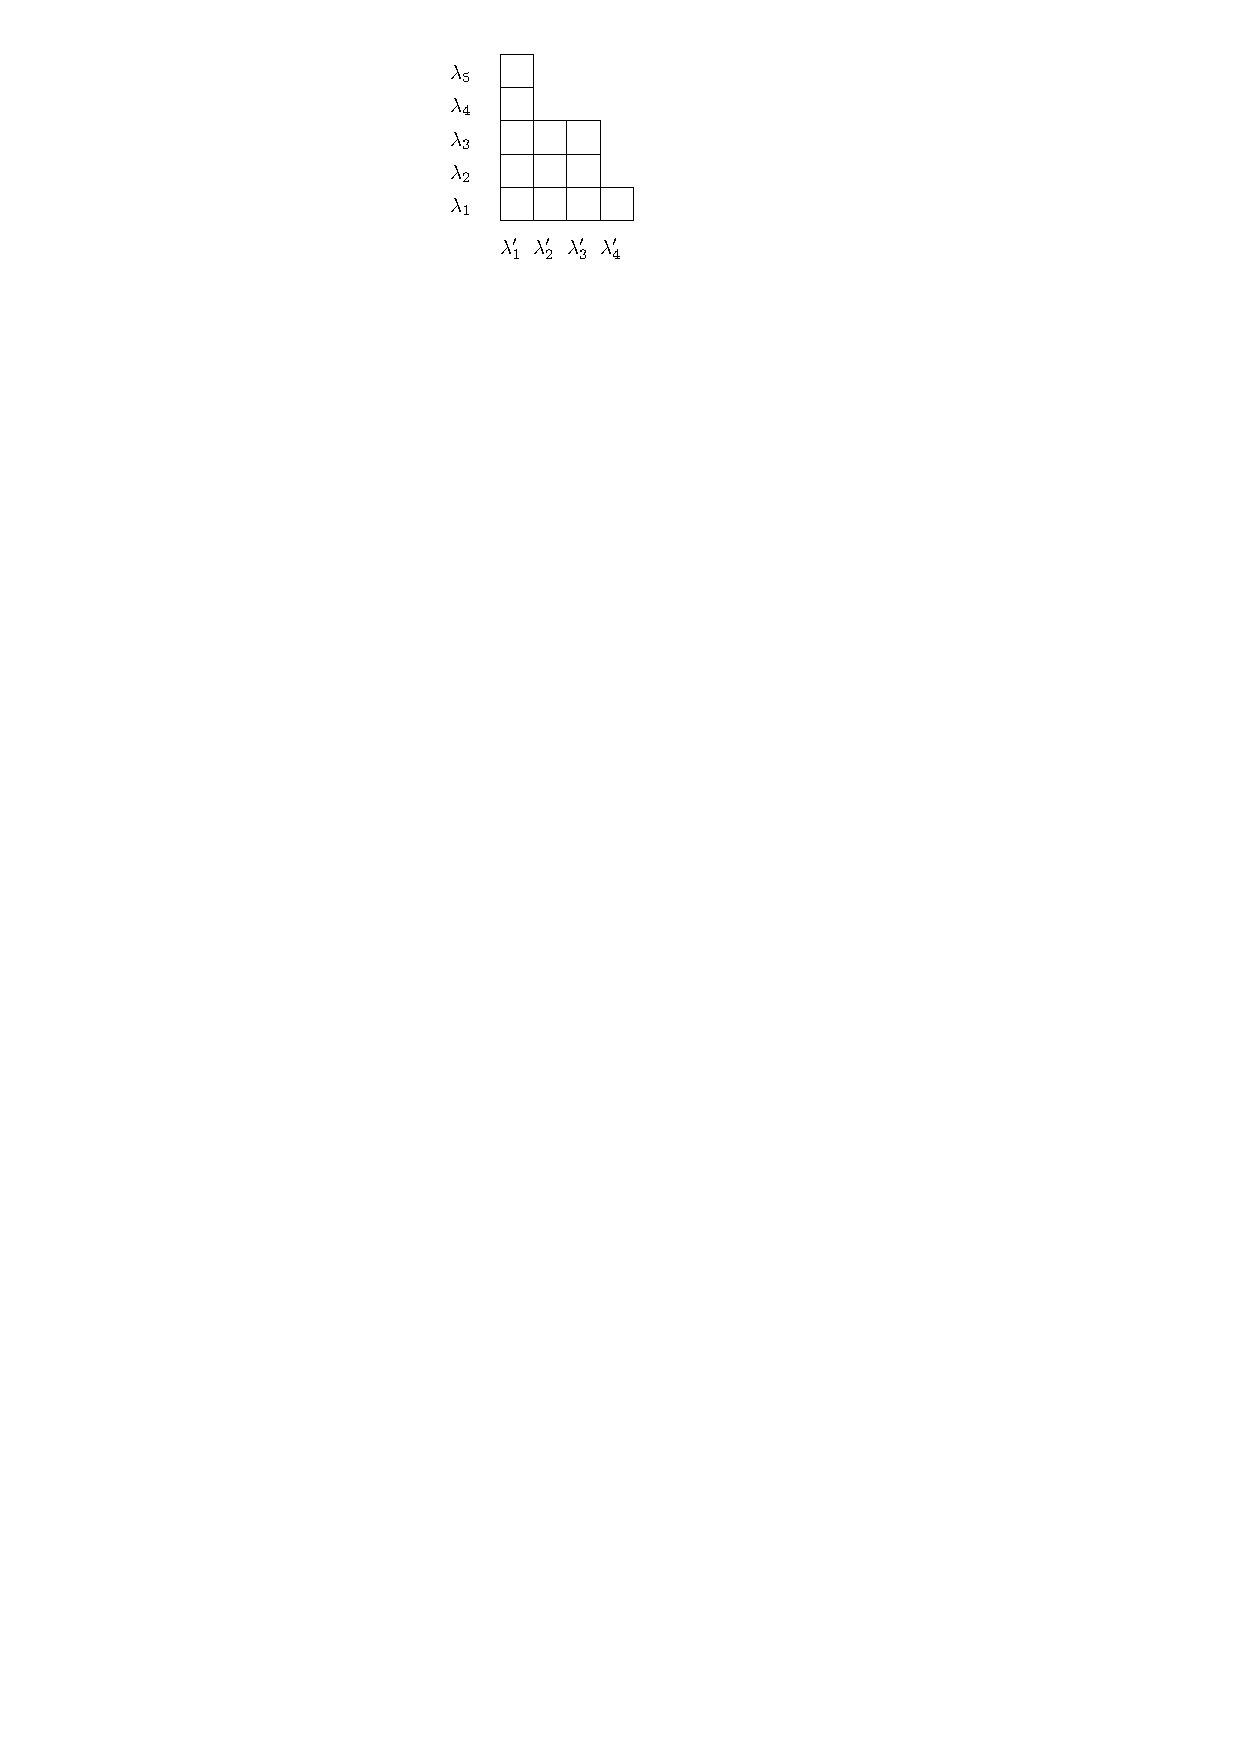
\includegraphics[width=0.15\linewidth]{Tableau3.pdf}
    \caption*{The diagram of $\lambda$}
\end{figure}}
\pause
The proof is based on a duality property of Macdonald polynomials, not known for interpolation polynomials.

\end{frame}

\begin{frame}{Application: Factorization property}
Fact: $$P^*_{1^k}(x_1,\dots,x_n;q,t)=e^*_k(x_1,\dots,x_n;t):=\sum_{ S\in {\llbracket n \rrbracket \choose k}} 
\prod_{i\in S}\left(x_i-\frac{t^{\#S^c\cap \llbracket i-1\rrbracket}}{t^{n-1}}\right),$$

\only<1>{
\textbf{\textcolor{uibred}{Example:}} For $n=3$ and $k=2$,
\smaller
$$
  e_2(x_1,x_2,x_3)=\left(x_1-\frac{1}{t^2}\right)\left(x_2-\frac{1}{t^2}\right)
  +\left(x_1-\frac{1}{t^2}\right)\left(x_3-\frac{t}{t^2}\right)+\left(x_2-\frac{t}{t^2}\right)\left(x_3-\frac{t}{t^2}\right).$$
}
\pause

\begin{theorem}[BD--Williams]
Let $\lambda$ be a partition with $\lambda_1>0$. For any subset 
$S \in {\llbracket n\rrbracket \choose \ell(\lambda)}$, we have
\begin{equation*}
  \sum_{\mu\in S_n(\lambda):\Supp(\mu)=S} f^*_\mu(x_1,\dots,x_n;1,t)=\prod_{i\in S}\left(x_i-\frac{t^{\#S^c\cap \llbracket i-1\rrbracket}}{t^{n-1}}\right)\prod_{2\leq i\leq \lambda_1}e^*_{\lambda'_i}.
\end{equation*}
As a consequence,
$$P^*_\lambda(x_1,\dots,x_n;q=1,t)=e^*_{\lambda'_1}\dots e^*_{\lambda'_{m}}.$$
\end{theorem}


\end{frame}

\begin{frame}{Sketch of the proof}
\textbf{Classic layers:}
When $q=1$, the weights in classic layers are probabilities.
\begin{figure}
    \centering
    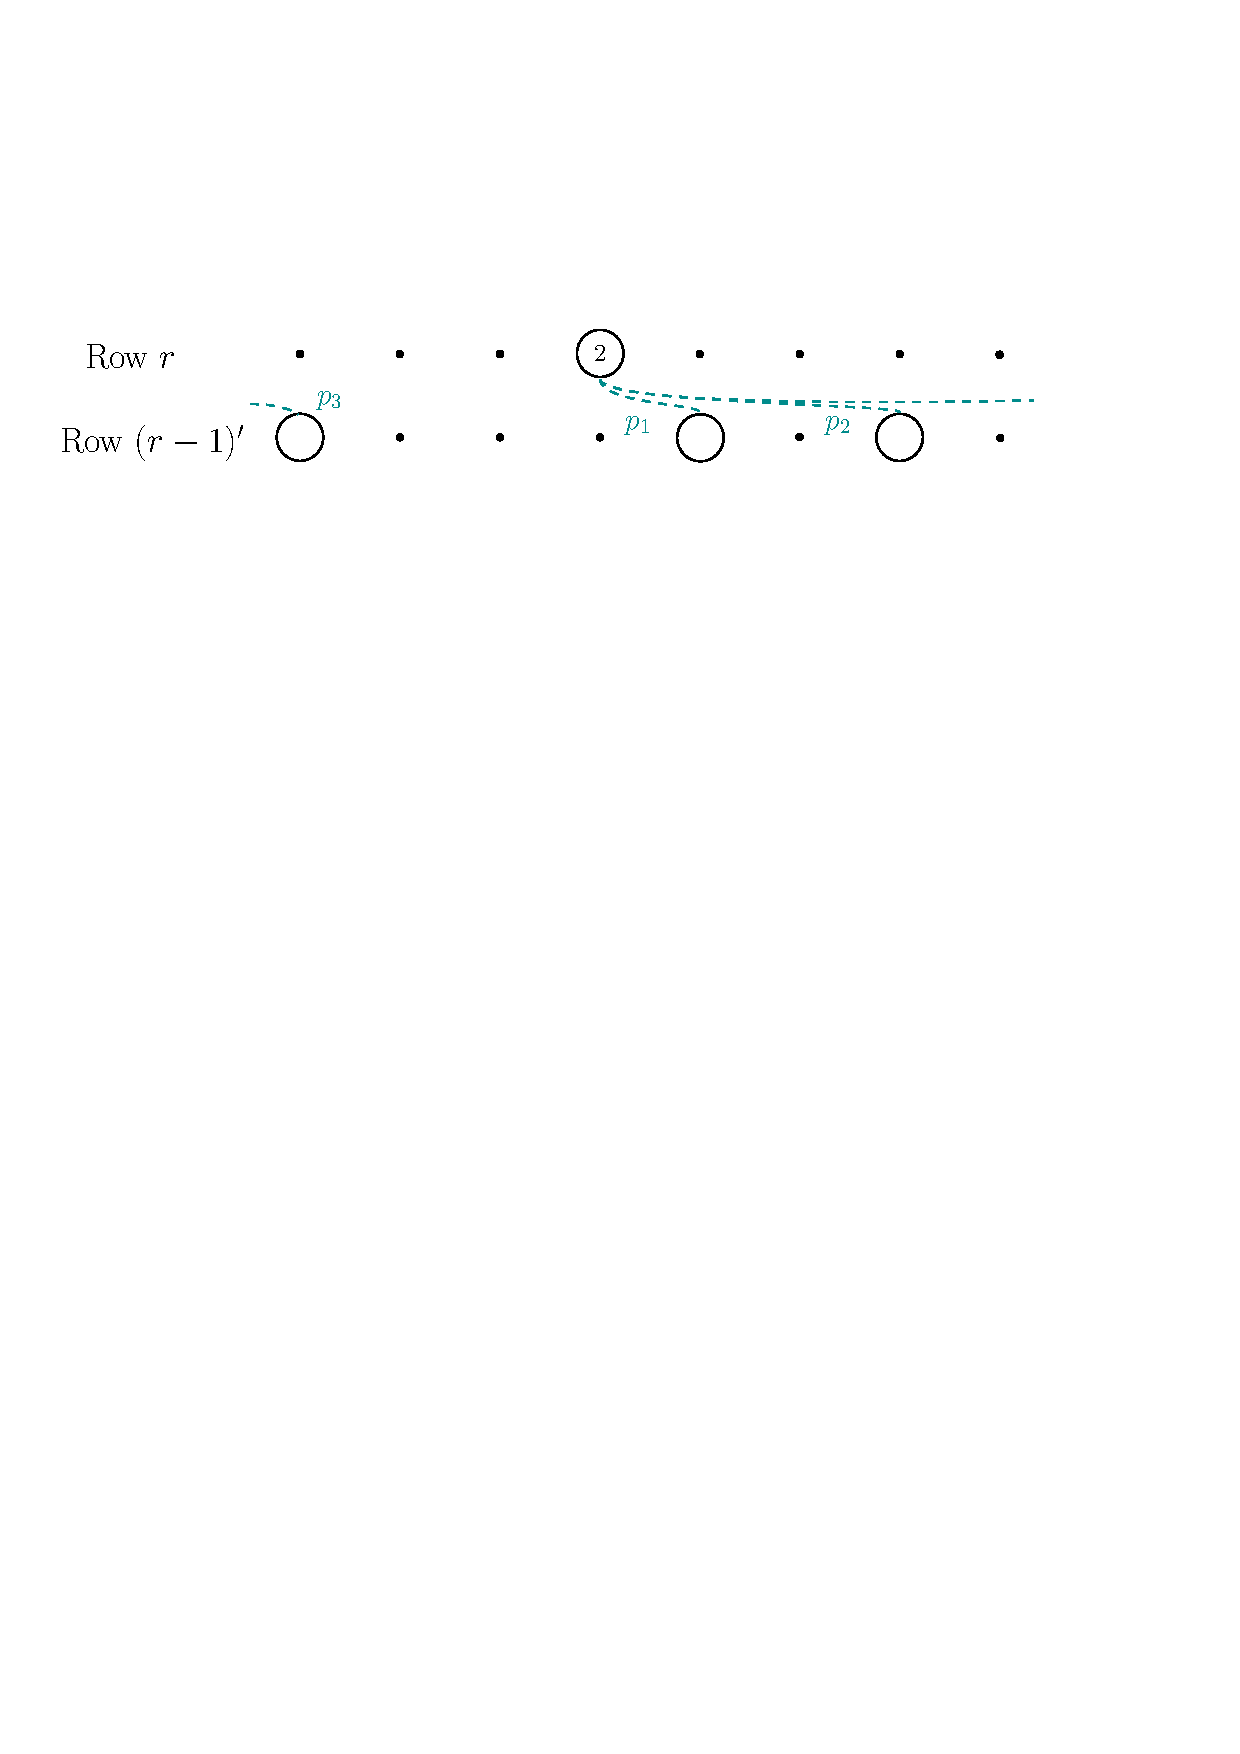
\includegraphics[width=0.7\linewidth]{q=1.pdf}
    \caption*{A ball in a classic row with three pairing possibilities.}
\end{figure}
$$\wt(p_1)=\frac{1-t}{1-t^3},\qquad \wt(p_2)=\frac{1-t}{1-t^3}t, \qquad\wt(p_3)=\frac{1-t}{1-t^3}t^2.$$
$$\wt(p_1)+\wt(p_2)+\wt(p_3)=1.$$
The composition in row $r$ is ``independent'' from the one in row $(r-1)'$.

\textbf{Signed layers:}
Start with the packed case for which these layers are trivial, and apply the Hecke operators.
\end{frame}





\end{document}

